% Autor: Manuel Lippert
% Physikalisches Praktikum

% Main-Datei für die Auswertung in TeX

% Struktur:
% Jedes Kapitel hat einen Input-File. Um Merge-Konflikte zu verhindern wird angeraten für jede 
% Datei eine eigene Tex Datei zu machen und sie im jeweiligen Kapitel zu importieren. Die in
% Input-Struktur dient zur besseren Übersicht und für mögliche Ordner, welche hier vorhanden sind. Die Zahlen vor den 
% Ordner dient zur Ordnung der einzelnen tex-Files nach Kapiteln


% Packages
\documentclass[paper=a4,bibliography=totoc,BCOR=10mm,twoside,numbers=noenddot,fontsize=11pt]{scrreprt}
\usepackage[ngerman]{babel}
\usepackage[T1]{fontenc}
\usepackage[latin1, utf8]{inputenc} %ä, ö, ü inbegriffen
\usepackage[babel,german=quotes]{csquotes} %For Quotes
\usepackage{lmodern}
\usepackage{graphicx}
\usepackage{nicefrac}
\usepackage{fancyvrb}
\usepackage{amsmath,amssymb,amstext}
\usepackage{siunitx}
\usepackage{url}
\usepackage[numbers]{natbib}
\usepackage{microtype}
\usepackage[format=plain]{caption}
\usepackage{physics}
\usepackage{titleref} 

% Zusätzliche Packages
\usepackage{geometry} % Verändert Seitengeometrie
\usepackage{anyfontsize} % Alle Schriftgrößen möglich machen
\usepackage[table]{xcolor} % Farbliche Gestaltung Tabellen
\usepackage{ifthen} % Für kompliziertere tex-Files
\usepackage[absolute,overlay]{textpos} %Textboxen
\usepackage{amsfonts} % Schriftarten
\usepackage{xstring} % Stringoperationen
\usepackage{tikz} % Zeichnungen
\usepackage{pdfpages} % Import von pdfs (Protokolle)
\usepackage{hyperref} % Verlinkungen im Dokument
\usepackage{subcaption} %Subfigure
\usepackage{makecell}

% Abschnittseinrückung und -abstand
% Die folgenden Zeilen sollen möglichst nicht verändert werden
\parindent 0.0cm
\parskip 0.8ex plus 0.5ex minus 0.5ex

% Anzahl und Größe von Gleitobjekten
% maximal 2 Objekte oben und unten
% erlaubt auch größere Bilder, welche die ganze Seite benötigen
% Die folgenden Zeilen sollen möglichst nicht verändert werden
\setcounter{bottomnumber}{2}
\setcounter{topnumber}{2}
\renewcommand{\bottomfraction}{1.}
\renewcommand{\topfraction}{1.}
\renewcommand{\textfraction}{0.}

%\sc und \bc veraltet. Daher: (20.09.2018)
\DeclareOldFontCommand{\sc}{\normalfont\scshape}{\@nomath\sc}
\DeclareOldFontCommand{\bf}{\normalfont\scshape}{\textbf}

% Verschiedenes
\pagestyle{headings}          % Der Seitenstil sollte möglichst nicht verändert werden
\graphicspath{{./Bilder/}}    % Der Pfad für die Abbildungen Abbildungen wird gesetzt
\VerbatimFootnotes            % \verb etc. auch in \footnotes mφglich

% Funktionen
\newcommand\tab[1][1cm]{\hspace*{#1}}
\newcommand{\vect}[1]{\boldsymbol{\mathbf{#1}}}
\newcolumntype{g}{>{\columncolor[rgb]{ .741,  .843,  .933}}l}
% Tiefgestellte Zahlen nicht kursiv
\catcode`_=\active
\newcommand_[1]{\ensuremath{\sb{\mathrm{#1}}}}

\begin{document}

    \nonfrenchspacing

    % 0. Kapitel Cover
    % 0. Cover

% Hier sind nur die Variablen und der Abschnitt Informationen (unten) zu bearbeiten der REst läuft automatisch ab (z.b Farbenänderung)

% Noch abänderbar nur ein Vorschlag
\newgeometry{top=30mm, bottom=20mm, inner=20mm, outer=20mm}
\thispagestyle{empty}

% Colors (Notability Colors)
\definecolor{Notablue}{HTML}{3498DB}		
\definecolor{Notared}{HTML}{CF366C}			
\definecolor{Notagreen}{HTML}{19B092}		
\definecolor{Notaorange}{HTML}{FA9D00}		
\definecolor{Notagrey}{HTML}{969696}		
\definecolor{Notalavendel}{HTML}{9DBBD8}	

% Boolean by default false. Für Absatz in der Überschrift
\newboolean{twoRows}
\newboolean{symbol}

% Funktions
\makeatletter
   \def\vhrulefill#1{\leavevmode\leaders\hrule\@height#1\hfill \kern\z@}
\makeatother
\newcommand*\ruleline[1]{\par\noindent\raisebox{.8ex}{\makebox[\linewidth]{\vhrulefill{\linethickness}\hspace{1ex}\raisebox{-.8ex}{#1}\hspace{1ex}\vhrulefill{\linethickness}}}}

% Variables
\def\schriftgrosse{40}
\def\linethickness{1,5pt}

\def\farbe{black}
\def\fach{PPBphys2}
\def\name{Manuel Lippert - Paul Schwanitz}
\def\titel{Förster-\\[0,5cm] Resonanzenenergietransfer \\[0,5cm] an biologischen Proben} % Absatz mit \\[0,5cm]
\def\bottom{WS2021/22}
\def\datum{28.09.2021}
\def\platz{NWI | BT5.3}
\def\betreuer{Chenyu Jin}

\def\teilnehmerm{Manuel Lippert}
\def\emailm{Manuel.Lippert@uni-bayreuth.de}
\def\teilnehmerp{Paul Schwanitz}
\def\emailp{Paul.Schwanitz@uni-bayreuth.de}

%\def\auswertp{}
%\def\messp{}
%\def\protop{}

\def\groupnr{11}

\begin{titlepage}
			
	\centering
	{\LARGE \sffamily {\textbf{\bottom}\par}}
	\vspace{2,5cm}
    {\fontsize{30}{0}\sffamily\ruleline{\textcolor{\farbe}{\textbf{\fach}}}\par}
    \vspace{6cm}
	{\Large\sffamily \ruleline{\name}\par}
		
	\IfSubStr {\titel} {\\[0,5cm]} {\setboolean{twoRows}{true}} {\setboolean{twoRows}{false}}
	
	\ifthenelse{\boolean{twoRows}}
		{
			\begin{textblock*}{21cm}(0cm,7,8cm) % {block width} (coords), centered		
				{\fontsize{\schriftgrosse}{0}\sffamily\textcolor{\farbe}{\textbf{\titel}}\par}
			\end{textblock*}
		}
		{
			\begin{textblock*}{21cm}(0cm,9cm) % {block width} (coords), centered		
				{\fontsize{\schriftgrosse}{0}\sffamily\textcolor{\farbe}{\textbf{\titel}}\par}
			\end{textblock*} 
		}
	
	% Choose Logo
	\ifthenelse {\equal{\farbe}{Notared}} {\def\logo{Bilder/Logo/UniBTNotared}}
		{\ifthenelse {\equal{\farbe}{Notagreen}} {\def\logo{Bilder/Logo/UniBTNotagreen}}
			{\ifthenelse {\equal{\farbe}{Notablue}} {\def\logo{Bilder/Logo/UniBTNotablue}}
				{\ifthenelse {\equal{\farbe}{Notaorange}} {\def\logo{Bilder/Logo/UniBTNotaorange}}
					{\ifthenelse {\equal{\farbe}{Notagrey}} {\def\logo{Bilder/Logo/UniBTNotagrey}}
						{\ifthenelse {\equal{\farbe}{Notalavendel}} {\def\logo{Bilder/Logo/UniBTNotalavendel}}	
							{\ifthenelse {\equal{\farbe}{black}} {\def\logo{Bilder/Logo/UniBT}}	
								{\def\logo{noLogo}}
							}
						}
					}
				}
			}
		}	

	\IfSubStr{\logo}{noLogo}{\setboolean{symbol}{false}}{\setboolean{symbol}{true}}
	
	% Gruppe
	\vspace{10cm}
	{\large\sffamily{Gruppe \groupnr}}
	
	%Logo
	\vfill

	\ifthenelse{\boolean{symbol}}
		{
			\begin{figure}[h]
			\begin{center}
				
				\includegraphics[width=2cm]{\logo}
				
			\end{center}
			\end{figure}
		}
	
\end{titlepage}

\restoregeometry

% Information
\chapter*{Informationen}
\label{chap:info}

\begin{tabular}{l l}

	{\textbf{Versuchstag}} \hspace{1cm} & \hspace{1cm} {\datum}\\[0,2cm]
	{\textbf{Versuchsplatz}} \hspace{1cm} & \hspace{1cm} {\platz}\\[0,2cm]
	{\textbf{Betreuer}} \hspace{1cm} & \hspace{1cm} {\betreuer}\\[1,2cm]
	{\textbf{Gruppen Nr.}} \hspace{1cm} & \hspace{1cm} {\groupnr}\\[0.2cm]
	% Für Fortgeschittenenen Praktikum
	{\textbf{Teilnehmer}} \hspace{1cm} & \hspace{1cm} {\teilnehmerm~(\emailm)}\\[0.2cm]
		     			  \hspace{1cm} & \hspace{1cm} {\teilnehmerp~(\emailp)}\\[0.2cm]
	% Für Grundpraktikum
	%{\textbf{Auswertperson}} \hspace{1cm} & \hspace{1cm} {\auswertp}\\[0.2cm]
	%{\textbf{Messperson}} \hspace{1cm} & \hspace{1cm} {\messp}\\[0.2cm]
	%{\textbf{Protokollperson}} \hspace{1cm} & \hspace{1cm} {\protop}\\[0.2cm]

\end{tabular}

    \thispagestyle{empty}
    \cleardoublepage
    \tableofcontents
    \cleardoublepage

    % 1. Kapitel Einleitung
    \chapter{Einleitung}
Die Spektroskopie basiert auf der Absorption von Licht und diese absorbierte Wellenlänge ist charakteristisch
für die zu untersuchende Verbindung. \\
Eine Art der Spektroskopie ist die \textbf{Fourier-Transformspektroskopie} (FTS).
Dieses Verfahren ist modern und wurde erst ab 1950 entwickelt. Hierbei 
wird ein Zweistrahl-Interferogramm der zu untersuchenden Probe aufgenommen und anschließend
erhält man das entsprechende Spektrum mithilfe der Fourier Transformation. Die Interferogramm-Intensitäten 
enthalten die gesamten Informationen des unbekannten Spektrums. \\

In unserem Versuch wird ein Michelson-Interferometer im sichtbaren Bereich als Zweistrahl
Interferogramm verwendet. Mit dessen Hilfe wird während dem Versuch eine Natrium Dampflampe,
eine Quecksilberhochdrucklampe und -niederdrucklampe untersucht. Anschließend kann man mithilfe
des aufgenommenen Spektrums die Kohärenzlänge, Wellenlänge und Linienbreite der untersuchten 
Linien bestimmen. 


    % 2.Kapitel Fragen zur Vorbereitung
    % 2. Fragen zur Vorbereitung

\chapter{Theoretischer Hintergrund}
\label{chap:theo}
Bevor wir uns zur Versuchsdurchführung und der Auswertung zuwenden wollen wir die Theorie von FRET näher besprechen. Dafür verwenden wir \citep{Anleitung} und \citep{Fluorescence} als Hauptquelle.

\section{FRET-Effekt}
\label{sec:dipolToFRET}
Um den FRET-Effekt zu beobachten, werden zwei Farbstoffe benötigt mit unterschiedlichen Absorptions- und Emissionsspektrum. Dabei muss sich das Emissionsspektrum des \textbf{\textit{Donor}}-Farbstoffs und das Absorptionsspektrum des \textbf{\textit{Akzeptor}}-Farbstoffs eine deutliche Überlappung aufzeigen (hellblauer Bereich in Abb. \ref{image:lappung}).\\

Durch Anregung des Donors wird das Molekül von einem Grundzustand $S_0$ in den ersten angeregten Zustand $S_1$ gebracht. Anzumerken ist aber, dass Moleküle anders, wie bei einzelnen Atomen, mehrere Energiezustände haben, darunter fällt die Energie des elektronischen Übergangs, der Schwingung und der Rotation (Gesamtenergie $E=E_{rot}+E_{vib}+E_{el}$). Das Vorhandensein von mehreren Energiezuständen hat zur Folge, dass sich Unterniveaus bilden in Fall von Molekülen entsteht ein \textit{Bandspektrum}.
\begin{center}
    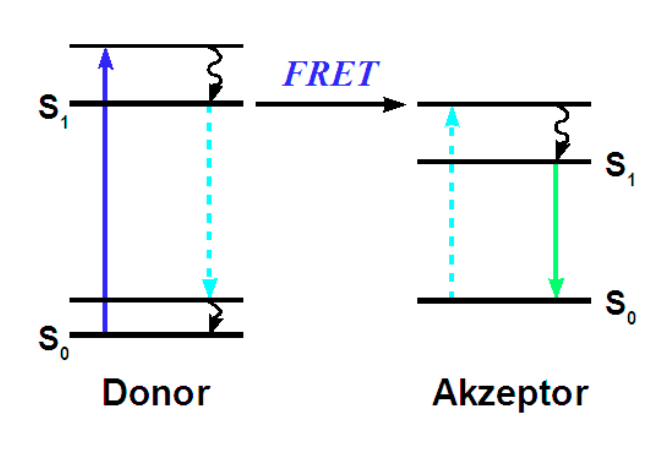
\includegraphics[scale=0.23]{FRET-Effekt.png}
    \captionof{figure}{FRET-Übergang \citep{Anleitung}}
    \label{image:FRET}
\end{center}
Durch Anregung eines Photons entsteht ein Übergang in das höhere Energieniveau $S_1$. Dieses koppelt sich an Vibrationen und verliert dabei ein Teil der Anregungsenergie des Photons. Nach der sogenannten Lebensdauer $\tau$ emittiert das Molekül spontan ein Fluoreszenzphoton und fällt in den Grundzustand $S_0$ zurück. Bei diesem Vorgang kommt es dann zur sogenannten \textit{Stokes-Verschiebung}, wodurch aufgrund des Energieverlusts die Wellenlänge des Fluoreszenzphotons höher ist als die des Anregungsphotons. Liegt nun die Wellenlänge des Fluoreszenzphotons im Absorptionsspektrum des Akzeptors geht die Anregungsenergie des Donors \textbf{\textit{strahlungslos}} auf den Akzeptor über, welcher wiederum durch Kopplung an Vibrationen ein Fluoreszenzphoton emittiert und in seinen Grundzustand zurückfällt. Diesen Vorgang nennt man \textbf{\textit{FRET-Effekt}} (siehe Abb. \ref{image:FRET}).
\newpage
\subsection*{Dipol-Dipol-Wechselwirkung und Fermis' goldene Regel}
Damit der Übergang der Energie strahlungslos vonstattengeht, muss es zu einer Dipol-Dipol.Wechselwirkung zwischen Donor und Akzeptor kommen. Dabei hängt die Effizienz des Energieübertrags von der Spektrenüberlappung, der Orientierung der Dipole und der Distanz der Farbstoffe verursacht vom Dipolfeld ab. Die Übergangswahrscheinlichkeit und die Effizienz des FRET-Effekts kann durch Fermis' goldene Regel angegeben werden:
\begin{gather}
    \abs{\left\langle \phi_{D}^* \phi_A \bigg \vert \frac{\kappa}{4\pi\epsilon_0} \frac{\mu_D\mu_A}{r^3} \bigg \vert \phi_D \phi_A^* \right\rangle }^2
\end{gather}
Dabei entspricht $\kappa$ dem winkelabhängigen Orientierungsfaktor der Dipole, $\epsilon_0$ der elektrischen Feldkonstante, $\mu_D$ dem elektrischen Dipolmoment des Donors und $\mu_A$ dem elektrischen Dipolmoment des Akzeptors. Die Abhängigkeit von $\frac{1}{r^3}$ kommt dabei von der Multipolentwicklung des Dipol-Moments und durch das quadrieren von Fermis' goldener Regel entsteht entsteht die $\frac{1}{r^6}$-Abhängigkeit in Gleichung \ref{eq:effizienz}. Die Effizienz des FRET-Effekts lässt sich dann wie folgt angeben:
\begin{gather}
    E = \frac{\text{Zahl der Energitransfers}}{\text{Zahl der Anregungen}} = \frac{k_{ET}}{k_F + k_{ET} + k_0} = \frac{R_F^6}{R_F^6+R^6}
    \label{eq:effizienz}
\end{gather}
Hierbei entspricht $R_F$ dem Försterradius und $R$ den Abstand zwischen den beiden Proben und $k_{ET}, k_F$ und $k_0$ den Raten der Energietransfers. Wenn der Abstand $R$ dem Försterradius $R_F$ entspricht, erhält man:
\begin{gather}
    E = \frac{R_F^6}{R_F^6+R^6} \overset{R = R_F}{=} \frac{1}{2}
\end{gather} 
Somit ist der Försterradius der Abstand zwischen den Proben, der einer Effizienz von 50\% entspricht.\\
Damit der FRET-Effekt auftritt sollte der Abstand $R$ zwischen Donor und Akzeptor ungefähr den Försterradius $R_F$ entsprechen. In unserem Versuch verwenden wir CFP und YFP Proben bei denen liegt der Försterradius bei einem Abstand von $R = \SI{4.9}{\nano\metre} = R_F$ \citep{Radius}. 
\subsection*{Abhängigkeit der Orientierung}
Besitzen der Donor und der Akzeptor eine feste Orientierung, verringern sich die Anzahl der Freiheitsgrade auf einen Freiheitsgrad, den Abstand. Womit die Effizienz nur vom Abstand $R$ abhängt.
\subsection*{Grenzfälle}
Beim Energietransfer sind mehrere Grenzfälle zu beachten, darunter fallen einen parallele oder eine orthogonale Orientierung der Moleküle zueinander. Bei paralleler Ausrichtung ist der Energietransfer am besten, während bei orthogonaler Ausrichtung keine Energie übertragen wird.
\subsection*{FRET-Effekt umgekehrt möglich?}
\begin{center}
    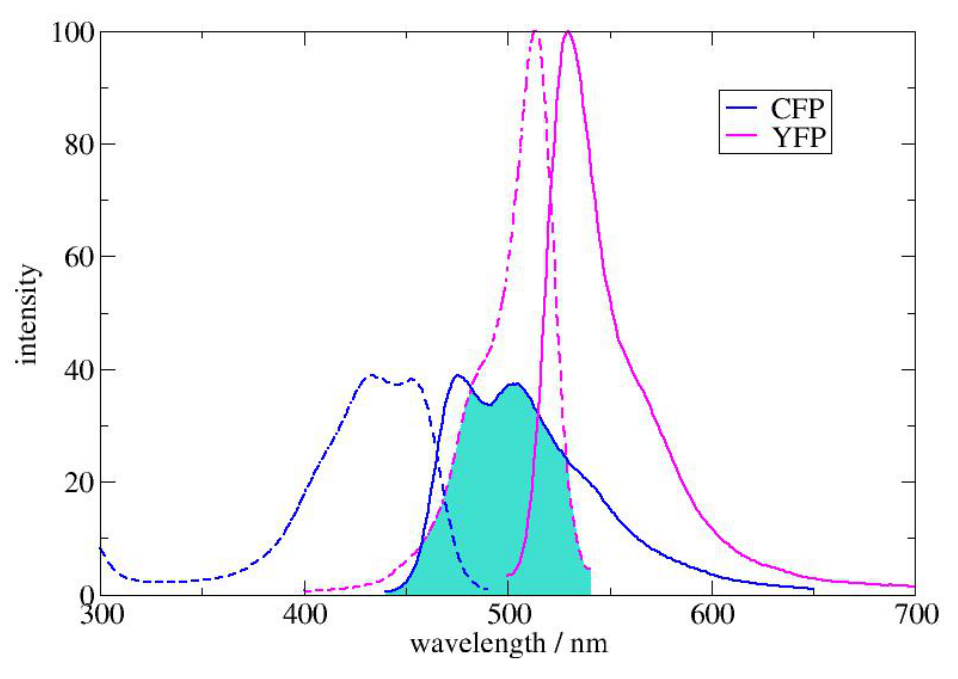
\includegraphics[scale=0.2]{Ueberlappung.png}
    \captionof{figure}{Anregungs- und Emissionsspektrum von CFP und YFP \citep{Anleitung}}
    \label{image:lappung}
\end{center}
Die Vorraussetzung für FRET ist die Überlappung des Emissionsspektrums des Donors und des Absorptionsspektrums des Akzeptors. Diese Vorraussetzung ist bei CFP als Donor und YFP als Akzeptor erfüllt (Durchgezogene blaue Linie zeigt deutliche Überlappung mit gestrichelter pinken Linie in Abb. \ref{image:lappung}). Vertauscht man aber die Rollen von CFP und YFP ist keinen Überlappung mehr gegeben (Durchgezogene pinke Linie schneidet gestrichelte blaue Linie nicht in Abb. \ref{image:lappung} und somit keine Überlappung). Damit ist in diesem Versuch keine FRET-Effekt mit YFP möglich.
\section{Crosstalk-Verunreinigungen}
\label{sec:verunreinigung}
\begin{center}
    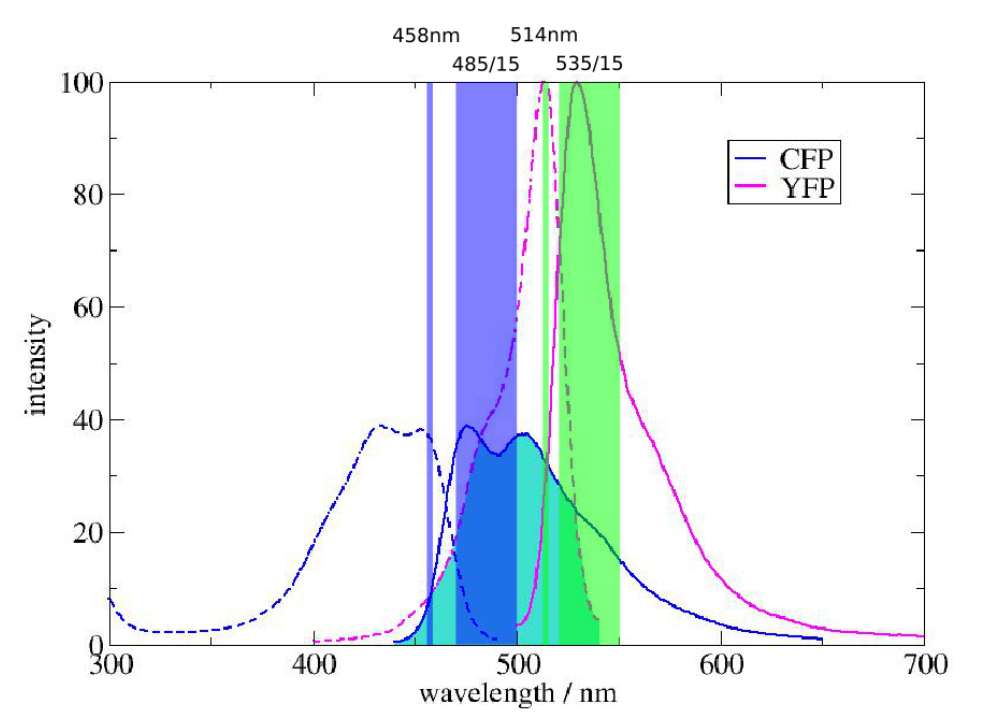
\includegraphics[scale=0.2]{Anregungslinien.png}
    \captionof{figure}{Anregungsbereiche von CFP und YFP \citep{Anleitung}}
    \label{image:anregung}
\end{center}
Die FRET-Intensität kann man nicht direkt messen, da sich der Anregungsbereich der Donors und Akzeptors teilweise überlappen (siehe Abb. \ref{image:anregung}). Somit wird bei einer Anregung des Donors auch der Akzeptor angeregt. Dies führt zu Verunreinigungen in der Messung der Emission des Akzeptors durch die teilweise Anregung. Um diesen Effekt zu korrigieren, misst man die Emission des Donors und die Emission des Akzeptors separat, womit man die Crosstalk Beiträge berechnen kann.
\section{Zeitkorrelierte Einzelphotonenzählung}
Allgemein ist zeitkorrelierte Einzelphotonenzählung (englisch time-correlated single photon counting, TCSPC) eine Technik, um sich zeitlich schnell ändernden Lichtintensitäten zu messen. Diese Messmethode kommt zum Einsatz bei der Messung von Fluoreszenzlebenszeit. Dabei wird die zu untersuchende Probe (Fluorophore) mithilfe von gepulsten Lichtbündel (Laser) angeregt. Die Detektion der Fluoreszenz erfolgt mit einem Photomultiplier, welcher einzelne Photonen registrieren können muss. Die Zeitmessung wird dann durch die Anregung des Laserpuls gestartet und das emittierte Photon stoppt diese. Die Messung wird wiederholt und die einzelnen Photonen werden, mit ihrer entsprechenden Zeit, in ein Histogramm eingetragen. Dieses zeigt einen exponentiellen Abfall der Fluoreszenzintensität nach der Anregung. Der Abfall ergibt sich dann mit der Formel:
\begin{gather}
    N(t) = N_0e^{-\frac{t}{\tau}}~\text{mit}~\frac{1}{\tau} = \sum^m_{i=1} k_i \xrightarrow{n~\text{Proben}} N(t) = \sum_{i=1}^n N_ie^{-\frac{t}{\tau_i}} 
\end{gather} 
Hierbei ist $\tau$ die Lebenszeit aus den $m$ einzelnen Zerfallsraten $k_i$ und $\tau_i$ die Lebenszeit der i-ten Probe mit entsprechender Amplitude $N_i$.\\
Das detektiert Signal hat dann die Form einer Faltung von dem exponentiellen Abfall und einer Gauß-Kurve (entsteht durch die IRF (Impulse Response Function) des Lasers), welches in Abb. \ref{image:abfall} zu sehen ist. Dabei ist der Teil bis zum Peak die IRF und danach der exponentielle Abfall.
\begin{center}
    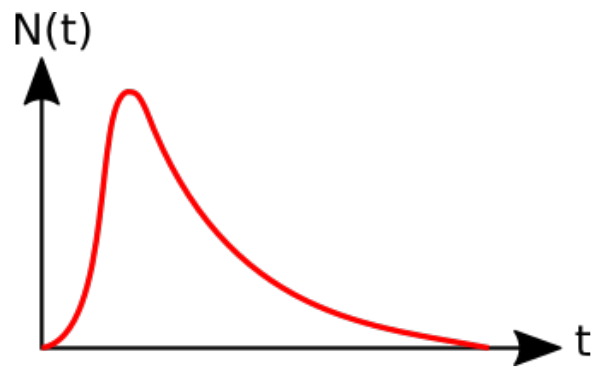
\includegraphics[scale = 0.3]{Abfall.png}
    \captionof{figure}{Verlauf der zeitkorrelierten Einzelphotonenzählung \citep{Anleitung}}
    \label{image:abfall}
\end{center}
\newpage
\subsection*{Störungen}
Bei dieser Messtechnik kann es allerdings zu Störungen kommen, welche das Ergbnis verfälschen.Dazu gehört das thermische Rauschen, wovon beinahe jedes Messgerät betroffen ist. Dies kann durch Kühlung des Messgerätes behoben werden.\\Weitere Störungsfaktoren, sogenannte ’Dark Counting’, sind \textit{Verstärkerrauschen}, \textit{'Afterpulsing'} und \textit{Pile-Up Effekt}.
\begin{itemize}
    \item[(1)] Das \textit{Verstärkerraschen} entsteht durch den angeschlossenen Photomultiplier und lässt sich mit einem Hochpassfilter lösen, da die Amplituden des Rauschens meist geringer sind als die Amplituden der eigentlichen Messung.
    \item[(2)] Beim \textit{'Afterpulsing'} registriert der Detektor nach dem Photonenereignis eine weiteres (fiktives) Ereignis. Behoben kann dies mit der richtigen Wahl des Detektors.
    \item[(3)] Der \textit{Pile-Up Effekt} entsteht durch den Umstand, dass eigentlich nur ein Photon pro Laserpuls mit der Probe wechselwirken kann. Bei mehreren Photonen registriert der Detektor nur das erste Photon, wodurch sich die gemessene Lebensdauer des Photons verringert. Verantwortlich für diesen Effekt ist die Totzeit des Detektors. In dieser Totzeit kann der Detektor kein weiteres Photon detektieren. Verringerung der Laserintensität kann dem Effekt entgegenwirken. \citep{Time}
\end{itemize} 
\newpage
\section{In diesem Versuch verwendete Proben}
\label{sec:proben}
Die verwendeten Proben in diesem Versuch werden mit einem Farbstoff markiert (Proben gehen kovalente Bindung mit Farbstoff-Molekül ein). Bei Anregung emittiert die Probe sichtbare Probe, was den Sachverhalt der Fluoreszenz darstellt.
\begin{center}
    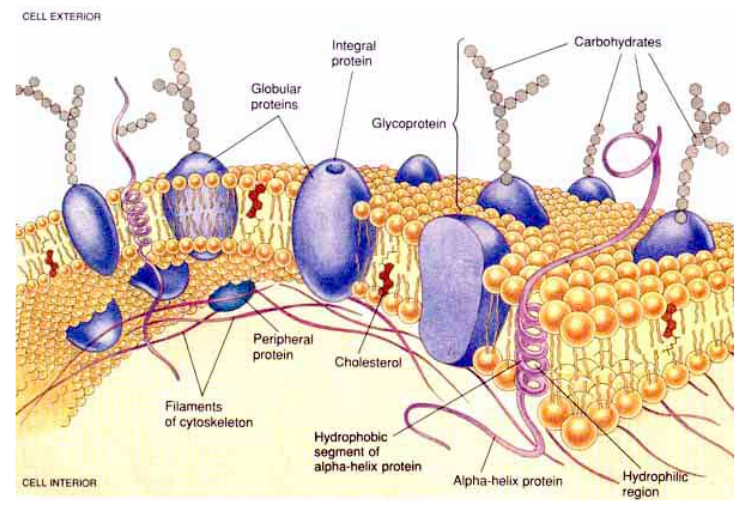
\includegraphics[scale=0.35]{Membran.png}
    \captionof{figure}{Skizze des Plasmamembran \citep{Anleitung}}
    \label{image:membran}
\end{center}
Die genutzte Zelle besitzen ein Plasmamembran, welches aus verschiedenen Lipiden aufgebaut ist (siehe Abb. \ref{image:membran}). Unterhalb der Lipiden sind ca. 30\% Phospholipide und Phosphatidylinositol(4,5)-Bisphosphat (PIP2). PIP2 ist besonders, denn es binden sich im Zellplasma vorhandenen Pleckstrin-Homologiedomäne (PH). In unserem Versuch wird dies verwendet, um CFP und YFP an Proteine mit einer solchen Pleckstrin-Homologiedomäne zu bindet. Durch die hohe Dichte an PIP2 binden sich viele CFP-PH und YFP-PH an das PIP2. Dies hat zur Folge, dass die Distanz zwischen YFP (Akzeptor) und CFP (Donor) gering genug ist, damit die Bedingung für FRET erfüllt ist.
\section{Photobleaching}
\label{sec:bleaching}
Das Photobleaching (dt. Bleichen) ist ein irreversibler Mechanismus, bei dem es zu einem Verlust der Fluoreszenzvon Fluorophoren kommt. Beim Bleaching wird das Fluorophor mit Licht bestrahlt, womit Photonen mit unterschiedlichen Energien auf die Probe treffen. Diese Photonen können vom Fluorophor absorbiert werden und es zu einem Übergang in einen angeregten Zustand (siehe Kapitel \ref{sec:dipolToFRET}). Durch Wechselwirkung zwischen dem angeregten Fluorophor und der Umgebung, kommt es zu einer kovalenten Änderung des Fluorophors, wodurch das Fluorophor seine Fluoreszenz verliert\\ Weiterhin kann man das Fluorophor mithilfe von Quenching (dt. Fluoreszenzlöschung) bleichen, dabei kommt es zu einer Abnahme der Fluoreszenz. Dieser Prozess ist aber zum Gegensatz zum Photobleaching reversibel. \citep{Bleach}
\section{Konfokalmikroskop}
\label{sec:konfokal}
Ein Konfokalmikroskop ist ein spezielles Lichtmikroskop, welches zu jedem Zeitpunkt nur einen Teil der Probe beleuchtet und genau dieser Bruchteil wird dann Stück für Stück abgerastert.
\subsection*{Funtionsweise}
\begin{center}
    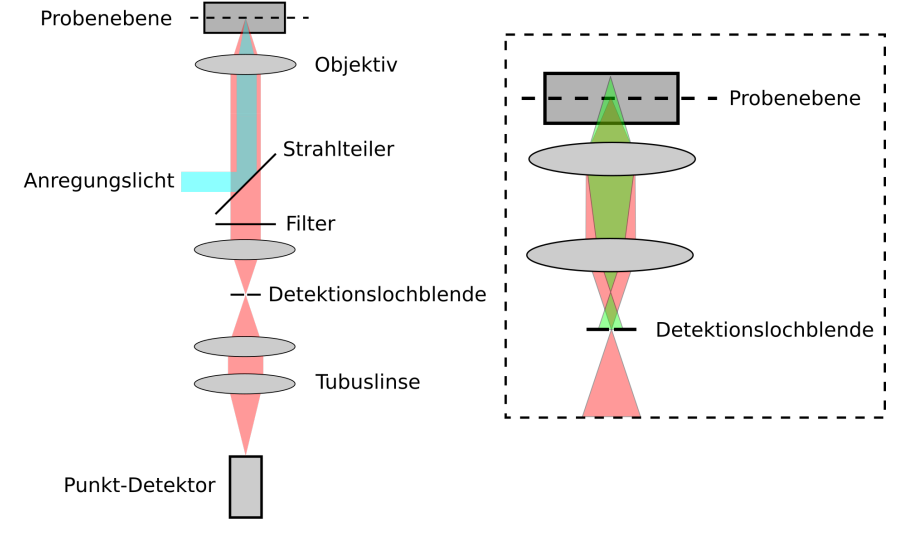
\includegraphics[scale=0.27]{Konfokallinsen.png}
    \captionof{figure}{Prinzipieller Aufbau eines Konfokalmikroskop \citep{Anleitung}}
    \label{image:konfokal}
\end{center}
In Abb. \ref{image:konfokal} wird der prinzipielle Aufbau eines Konfokalmikroskop gezeigt. Dabei wird der Anregungsstrahl (blau in \ref{image:konfokal}) durch einen Strahlenteiler reflektiert und durch eine Linse gebündelt mit dem Brennpunkt auf der Probe. Von der Probe wird dann der sogenannte Detektionsstrahl (rot in \ref{image:konfokal}) ausgesendet. Dieser Strahl wird durch die oberste Linse parallelisiert und trifft auf den Strahlenteiler, der den Strahl transmittieren lässt. Nach dem Strahlenteiler kann ein Filter eingebaut werden, welcher die störenden Wellenlängen herausfiltert. Nach dem Filter befindet sich eine weitere Linse und die Detektionslochblende, welche das Detektionsvolumen auf einen kleinen Bereich einschränkt. Dies bedeutet das Strahlen aus einem hinteren Bereich der Probe nicht zum Detektor gelangen. Nach der Blende trifft der Detektionsstrahl auf die erste Tubuslinse. Diese parallelisiert den Strahl erneut und die zweite Tubuslinse fokussiert ihn auf den Punkt-Detektor. Der Punkt-Detektor registriert dann die einzelnen Photonen.
\subsection*{Vor und Nachteile}
\begin{itemize}
    \item[\textcolor{green}{\textbf{+}}] Unerwünschtes Hintergrundrauschen (z.B. Streulicht) reduzierbar auf ein Minimum und bessere Auflösung zum Vergleich zu konventionellen Mikroskopen wegen der Detektionslochblende
    \item[\textcolor{red}{\textbf{-}}] Detektionslochblende kann Beugungserscheinungen verursachen, was die Auflösung begrenzt
\end{itemize}
Als Alternative zum Konfokalmikroskop kann das Laser-Scanning-Microscope verwendet werden, welches ohne die Detektionslochblende auskommt und eine höhere Auflösung besitzt.

    % 3.Kapitel Protokoll
    
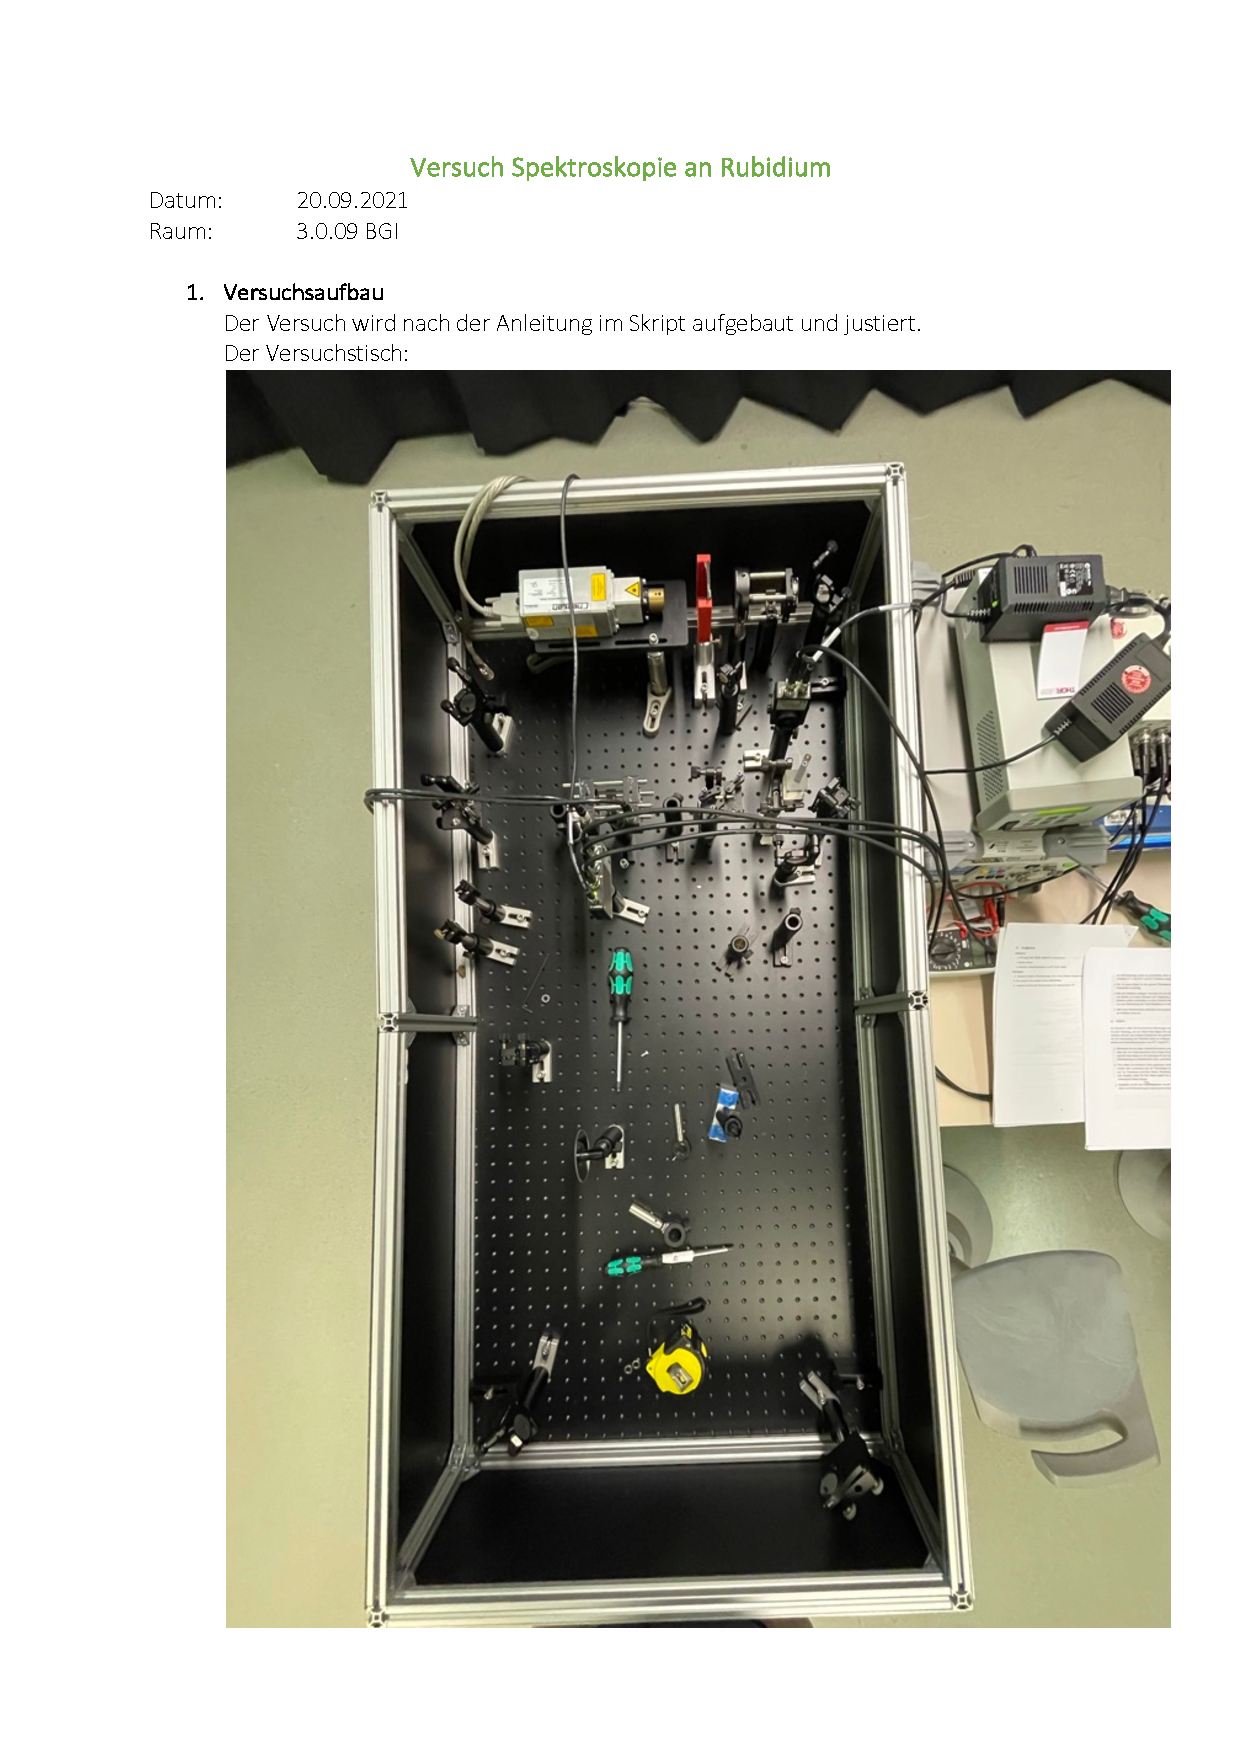
\includepdf[pages=1,landscape = false, offset=0 -25mm, scale=0.71,pagecommand ={\thispagestyle{empty}}\chapter{Messprotokoll}]{Protokoll_Messung/Protokoll.pdf}

\includepdf[pages={2-4},scale=0.8,pagecommand ={\thispagestyle{plain}}]{Protokoll_Messung/Protokoll.pdf}

    % 4.Kapitel Versuchsauswertung
    % 4. Versuchsauswertung

\chapter{Auswertung und Diskussion}
\label{chap:versuchsauswertung}

% Text

% Input der Teilauswertung je nach Produktion der Nebendateien ohne Ordner
% Teilauswertung 1

\section{Mittelung und Fouriertransformation}
\label{sec:mittelungAndTrafo}

\paragraph{a)}\textbf{Experimentelle Bestimmung der Fourierentwicklungskoeffizienten}

Im Folgenden wird die Fourierentwicklungskoeffizienten der Sinus, Rechteck und Dreiecksschwingung experimentell bestimmt. Dazu werden die einzelnen Peaks im Fourierspektrum mithilfe von einem Python-Skript (argelextrma Modul aus scipy.signal Paket ermittelt, welche dann den Wert der Fourierentwicklungskoeffizienten für diese Frequenz darstellen. Beachtet werden nur ungerade Vielfache der eingestellten Frequenz. Dies folgt aus Kapitel \ref{sec:fourierseries} bei der nur ungerade Vielfache in der Reihenentwicklung von Rechteck und Dreieckschwingung vorkommen. Die Daten der Amplitude $A$ wurden dabei in dB aufgenommen. Für die Umrechnung der Amplitude in dB zu Volt wird die Gleichung (\ref{eq:spannungpegel}) aus Kapitel \ref{sec:pegel} nach der Spannung $U$ aufgelöst und erhält:
\begin{gather}
    L_U = 20 \log_{10}\left(\frac{U}{U_0}\right)~\Leftrightarrow~U = U_0 \cdot 10^{\frac{L_U}{20}}
    \label{eq:umpegel}
\end{gather}
Zu beachten ist noch, dass die Spannung $U$ die gemessene Effektivspannung ist. Diese Effektivspannung muss mit dem Faktor für die Sinusschwingung aus Kapitel \ref{sec:fourierseries} umgewandelt werden, da die Fourierreihe der jeweiligen Schwingung aus Sinusschwingungen besteht. Die verwendeten Formeln sind dann:
\begin{gather}
    U = U_0 \cdot 10^{\frac{L_U}{20}} \cdot \sqrt{2}  ~\text{mit}~U_0=1\,\text{V}
    \label{eq:umrechnung}
\end{gather}
Die Auswertung ergibt dann Tabelle \ref{tab:fourierkoeff}, in welcher man gut erkennen kann, dass die gemessenen Werte nicht weit von der Theorie abweichen. Dafür wurde die betragsmässige Differenz $\Delta A = \abs{A_{Mess}-A_{Theo}}$ zusätzlich berechnet und graphisch in Abbildung \ref{image:residuum} mit den Fourierspektren der Schwingungen dargestellt. Dabei wurden die theoretischen Werte mit Gleichung (\ref{eq:umpegel}) umgerechnet mit $U = U_{Theo}/\sqrt{2}$. Bei genauerer Betrachtung fällt auf, dass die Kurven für die Rechteckschwingung und der Dreieckschwingung bis zu einer Frequenz $f=9$\,kHz einen ähnlichen Verlauf haben. Danach steigt $\Delta A$ für die Rechteckschwingung stetig bis zu einem Maximum bei 100\,kHz an währenddessen die Dreieckschwingung weiterhin nahe bei 0\,$\mu$V bleibt. Dies kann durch Rauschen in der Messapparatur verursacht worden sein.
\newpage
\begin{center}
    %\textbf{Sinus}\\[0,2cm]
    %\begin{tabular}{l | c | c c c}
    %    $k$ & $f$/kHz &   $A_{Mess}$/V & $A_{Theo}$/V & $\Delta A$/V\\
    %    \hline
    %    1 & 1 &  1,0024 & 1,0000 & 0,0024\\
    %\end{tabular}\\[0,5cm]
    \begin{tabular}{l | c | c c r | c c r}
        \multicolumn{2}{c}{} & \multicolumn{3}{c}{\textbf{Rechteck}} & \multicolumn{3}{c}{\textbf{Dreieck}}\\
        $k$ & $f$/kHz  &   $A_{Mess}$/V & $A_{Theo}$/V & $\Delta A$/$\mu$V  &   $A_{Mess}$/V & $A_{Theo}$/V & $\Delta A$/$\mu$V\\
        \hline
        1  &       1 &  1,276204 &  1,273240 & 2964,00 & 0,812606 &  0,810569 & 2036,48 \\
        2  &       3 &  0,425216 &  0,424413 &  803,00 & 0,090246 &  0,090063 &  183,15 \\
        3  &       5 &  0,254976 &  0,254648 &  328,00 & 0,032489 &  0,032423 &   66,12 \\
        4  &       7 &  0,181976 &  0,181891 &   85,00 & 0,016573 &  0,016542 &   31,10 \\
        5  &       9 &  0,141379 &  0,141471 &   92,00 & 0,009979 &  0,010007 &   27,96 \\
        6  &      11 &  0,115513 &  0,115749 &  236,00 & 0,006700 &  0,006699 &    1,16 \\
        7  &      13 &  0,097574 &  0,097942 &  367,00 & 0,004805 &  0,004796 &    8,75 \\
        8  &      15 &  0,084397 &  0,084883 &  486,00 & 0,003604 &  0,003603 &    1,51 \\
        9  &      17 &  0,074300 &  0,074896 &  596,00 & 0,002806 &  0,002805 &    1,31 \\
        10 &      19 &  0,066309 &  0,067013 &  704,00 & 0,002247 &  0,002245 &    1,82 \\
        11 &      21 &  0,059820 &  0,060630 &  811,00 & 0,001853 &  0,001838 &    1,48 \\
        12 &      23 &  0,054445 &  0,055358 &  913,00 & 0,001530 &  0,001532 &    2,60 \\
        13 &      25 &  0,049915 &  0,050930 & 1014,00 & 0,001298 &  0,001297 &    1,31 \\
        14 &      27 &  0,046045 &  0,047157 & 1112,00 & 0,001116 &  0,001112 &    4,53 \\
        15 &      29 &  0,042696 &  0,043905 & 1209,00 & 0,000963 &  0,000964 &    1,13 \\
        16 &      31 &  0,039764 &  0,041072 & 1308,00 & 0,000846 &  0,000843 &    2,17 \\
        17 &      33 &  0,037185 &  0,038583 & 1398,00 & 0,000737 &  0,000744 &    7,77 \\
        18 &      35 &  0,034885 &  0,036378 & 1493,00 & 0,000654 &  0,000662 &    8,18 \\
        19 &      37 &  0,032824 &  0,034412 & 1588,00 & 0,000591 &  0,000592 &    0,72 \\
        20 &      39 &  0,030967 &  0,032647 & 1680,00 & 0,000521 &  0,000533 &   12,02 \\
        21 &      41 &  0,029284 &  0,031055 & 1771,00 & 0,000480 &  0,000482 &    1,84 \\
        22 &      43 &  0,027747 &  0,029610 & 1863,00 & 0,000433 &  0,000438 &    5,67 \\
        23 &      45 &  0,026338 &  0,028294 & 1956,00 & 0,000395 &  0,000400 &    4,88 \\
        24 &      47 &  0,025044 &  0,027090 & 2046,00 & 0,000362 &  0,000367 &    4,84 \\
        25 &      49 &  0,023854 &  0,025984 & 2130,00 & 0,000335 &  0,000338 &    2,90 \\
        26 &      51 &  0,022747 &  0,024965 & 2218,00 & 0,000312 &  0,000312 &    0,68 \\
        27 &      53 &  0,021718 &  0,024023 & 2305,00 & 0,000280 &  0,000289 &    8,32 \\
        28 &      55 &  0,020760 &  0,023150 & 2390,00 & 0,000264 &  0,000268 &    4,02 \\
        29 &      57 &  0,019863 &  0,022338 & 2475,00 & 0,000255 &  0,000249 &    5,43 \\
        30 &      59 &  0,019024 &  0,021580 & 2557,00 & 0,000237 &  0,000233 &    3,97 \\
        31 &      61 &  0,018230 &  0,020873 & 2642,00 & 0,000218 &  0,000218 &    0,44 \\
        32 &      63 &  0,017489 &  0,020210 & 2721,00 & 0,000205 &  0,000204 &    0,45 \\
        33 &      65 &  0,016786 &  0,019588 & 2802,00 & 0,000194 &  0,000192 &    1,69 \\
        34 &      67 &  0,016126 &  0,019004 & 2878,00 & 0,000181 &  0,000181 &    0,39 \\
        35 &      69 &  0,015501 &  0,018453 & 2951,00 & 0,000170 &  0,000170 &    0,61 \\
    \end{tabular}
    \begin{tabular}{l | c | c c r | c c r}
        \multicolumn{2}{c}{} & \multicolumn{3}{c}{\textbf{Rechteck}} & \multicolumn{3}{c}{\textbf{Dreieck}}\\
        $k$ & $f$/kHz  &   $A_{Mess}$/V & $A_{Theo}$/V & $\Delta A$/$\mu$V  &   $A_{Mess}$/V & $A_{Theo}$/V & $\Delta A$/$\mu$V\\
        \hline  
        36 &      71 &   0,014909 &  0,017933 &  3024,00 & 0,000164 &  0,000161 &   3.33 \\
        37 &      73 &   0,014344 &  0,017442 &  3097,00 & 0,000156 &  0,000152 &   4.20 \\
        38 &      75 &   0,013814 &  0,016977 &  3163,00 & 0,000145 &  0,000144 &   1.37 \\
        39 &      77 &   0,013305 &  0,016536 &  3230,00 & 0,000134 &  0,000137 &   3.04 \\
        40 &      79 &   0,012825 &  0,016117 &  3292,00 & 0,000133 &  0,000130 &   3.28 \\
        41 &      81 &   0,012368 &  0,015719 &  3351,00 & 0,000129 &  0,000124 &   5.11 \\
        42 &      83 &   0,011932 &  0,015340 &  3408,00 & 0,000122 &  0,000118 &   4.17 \\
        43 &      85 &   0,011522 &  0,014979 &  3457,00 & 0,000116 &  0,000112 &   4.29 \\
        44 &      87 &   0,011128 &  0,014635 &  3506,00 & 0,000111 &  0,000107 &   4.24 \\
        45 &      89 &   0,010757 &  0,014306 &  3549,00 & 0,000100 &  0,000102 &   2.13 \\
        46 &      91 &   0,010407 &  0,013992 &  3585,00 & 0,000106 &  0,000098 &   8.08 \\
        47 &      93 &   0,010077 &  0,013691 &  3614,00 & 0,000098 &  0,000094 &   4.35 \\
        48 &      95 &   0,009761 &  0,013403 &  3641,00 & 0,000090 &  0,000090 &   0.64 \\
        49 &      97 &   0,009467 &  0,013126 &  3659,00 & 0,000089 &  0,000086 &   2.70 \\
        50 &      99 &   0,009193 &  0,012861 &  3668,00 & 0,000088 &  0,000083 &   5.51 \\
        51 &     101 &   0,008936 &  0,012606 &  3671,00 & 0,000087 &  0,000079 &   7.23 \\
        52 &     103 &   0,008699 &  0,012362 &  3662,00 & 0,000089 &  0,000076 &  13,00 \\
        53 &     105 &   0,008479 &  0,012126 &  3647,00 & 0,000079 &  0,000074 &   5.97 \\
        54 &     107 &   0,008283 &  0,011899 &  3617,00 & 0,000084 &  0,000071 &  13,70 \\
        55 &     109 &   0,008101 &  0,011681 &  3580,00 & 0,000081 &  0,000068 &  13,08 \\
        56 &     111 &   0,007937 &  0,011471 &  3534,00 & 0,000080 &  0,000066 &  13,76 \\
        57 &     113 &   0,007803 &  0,011268 &  3465,00 & 0,000077 &  0,000063 &  13,08 \\
        58 &     115 &   0,007687 &  0,011072 &  3385,00 & 0,000076 &  0,000061 &  15,02 \\
        59 &     117 &   0,007586 &  0,010882 &  3297,00 & 0,000080 &  0,000059 &  20,31 \\
        60 &     119 &   0,007514 &  0,010699 &  3186,00 & 0,000076 &  0,000057 &  18,57 \\
        61 &     121 &   0,007456 &  0,010523 &  3066,00 & 0,000075 &  0,000055 &  19,14 \\
        62 &     123 &   0,007423 &  0,010352 &  2929,00 & 0,000078 &  0,000054 &  24,34 \\
    \end{tabular}  
    \captionof{table}{Vergleich Fourierentwicklungskoeffizienten in Theorie und Praxis}
    \label{tab:fourierkoeff}
\end{center}
\begin{center}
    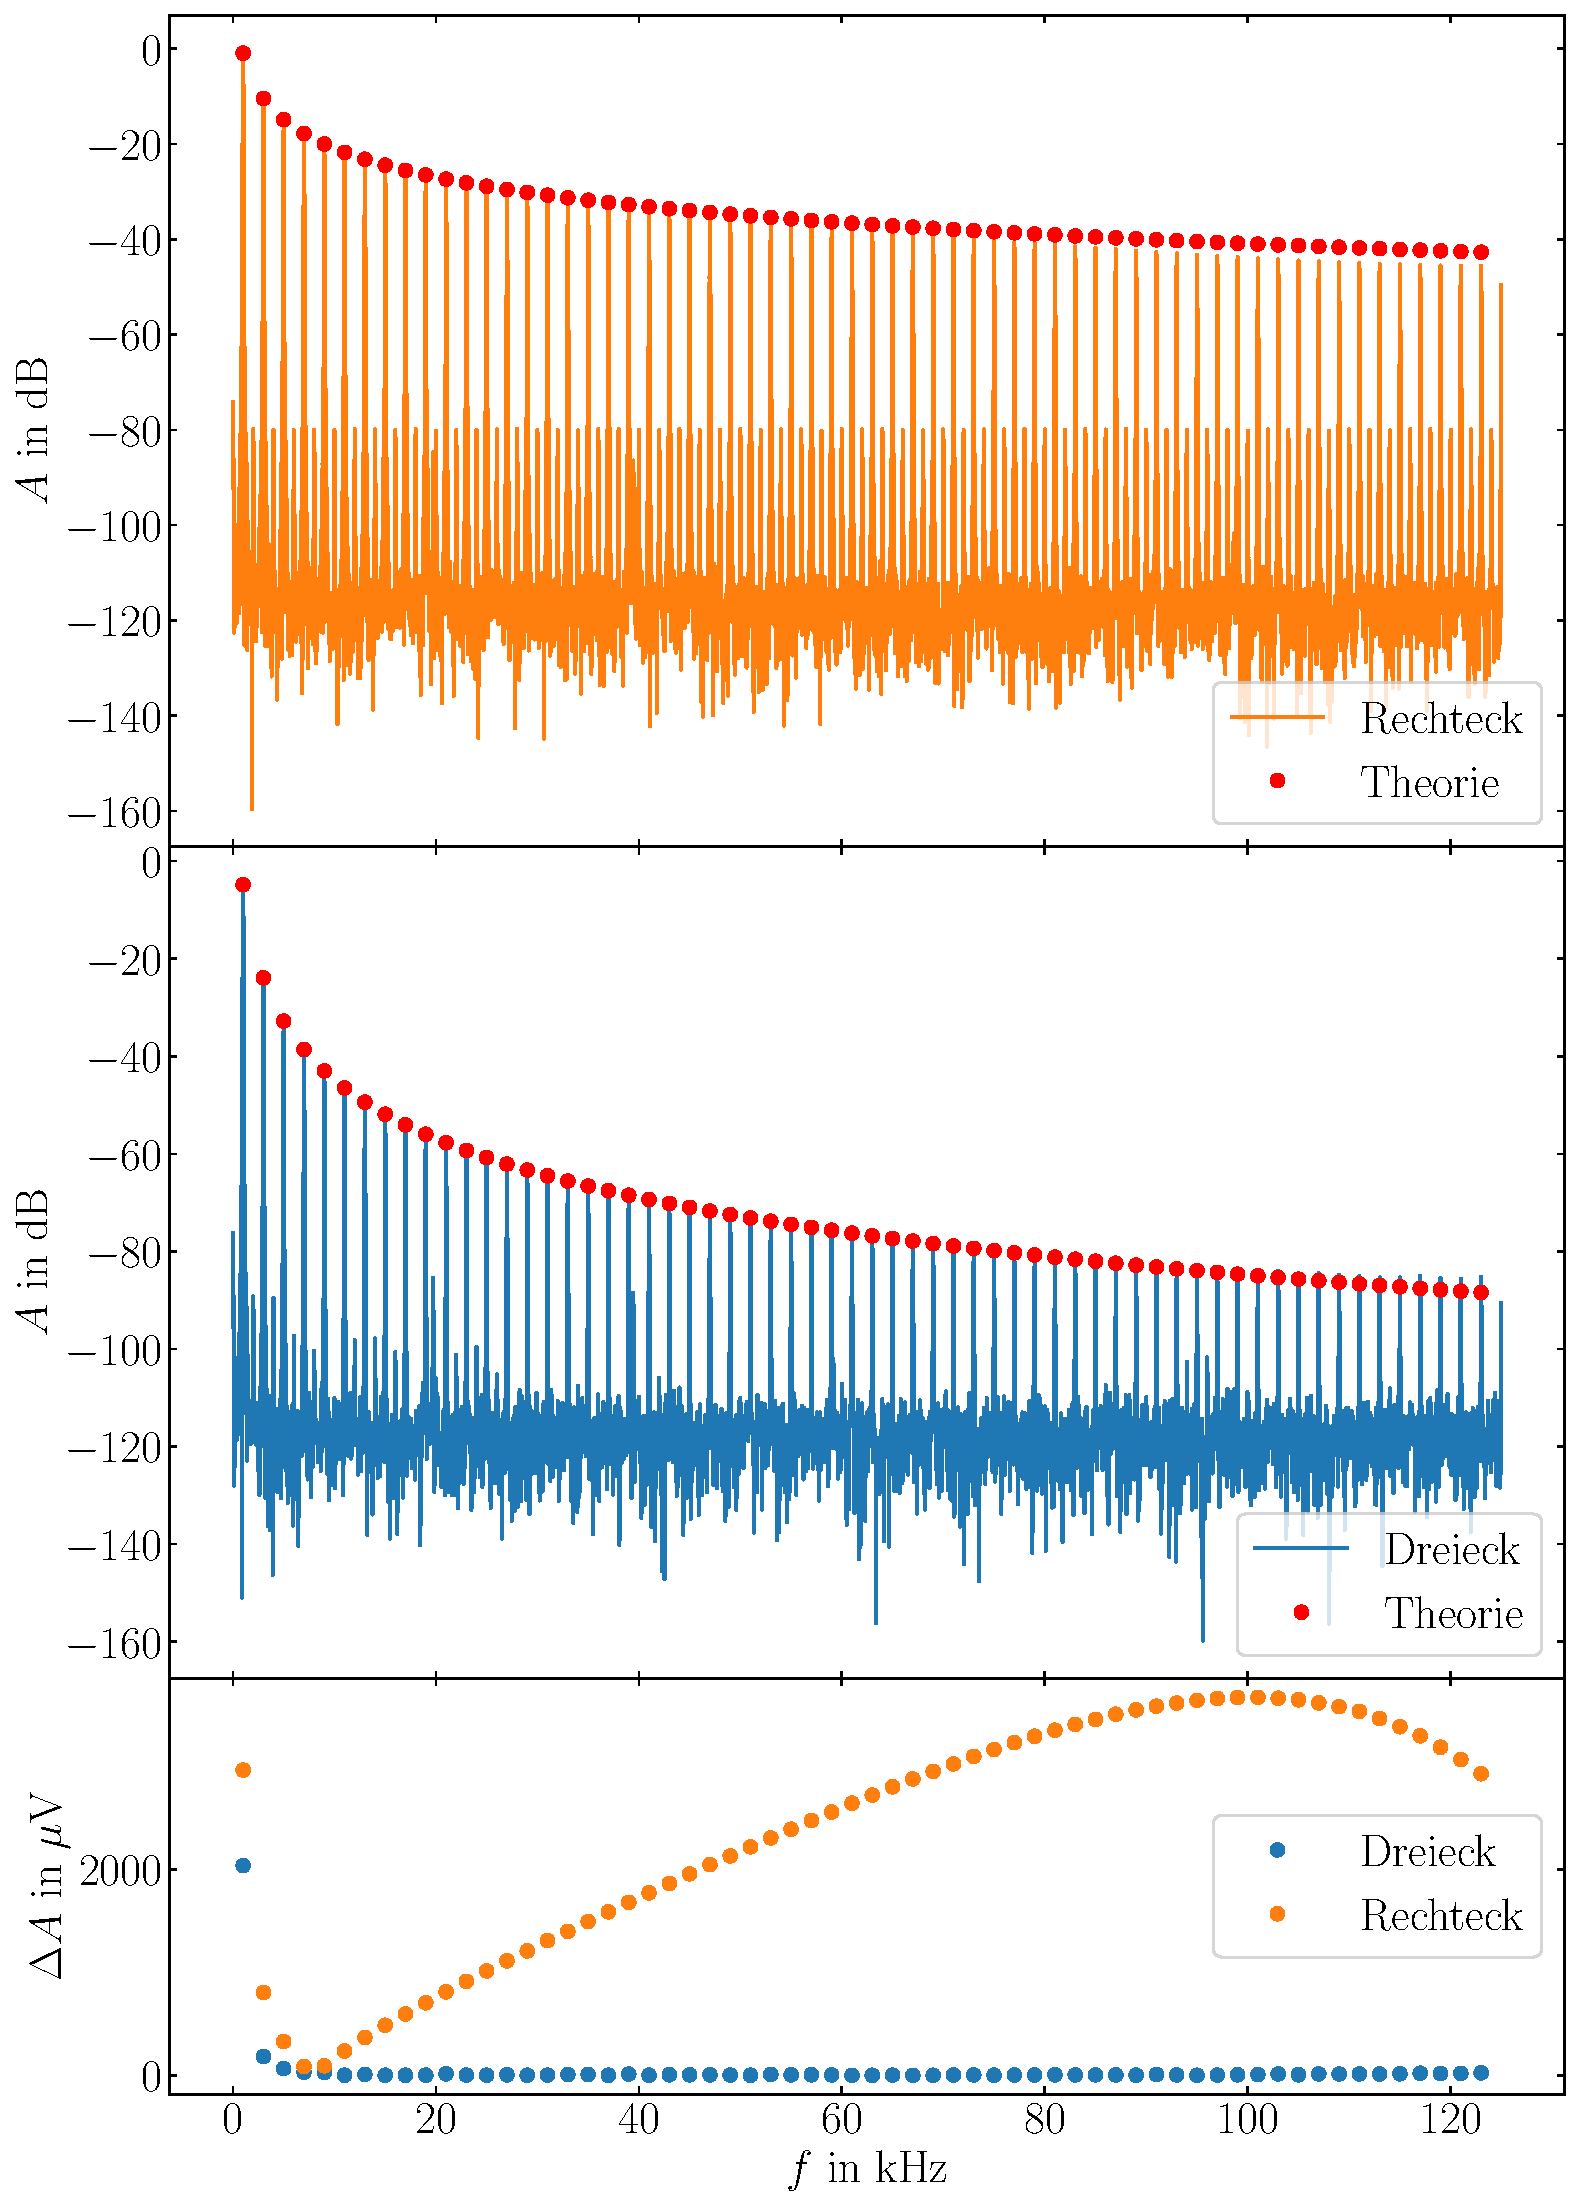
\includegraphics[scale = 0.5]{Manuel/41/Residuum.pdf}
    \captionof{figure}{Betragsmässige Differenz der Messwerte und Theorie mit den jeweiligen Fourierspektrum der Schwingungsform mit Theorie}
    \label{image:residuum}
\end{center}


\newpage
\paragraph{b)}\textbf{Fourierspektrum Sinusschwingung}

Dieser Teil behandelt das Fourierspektrum der Sinusschwingung bei 1\,V Amplitude.
\begin{center}
    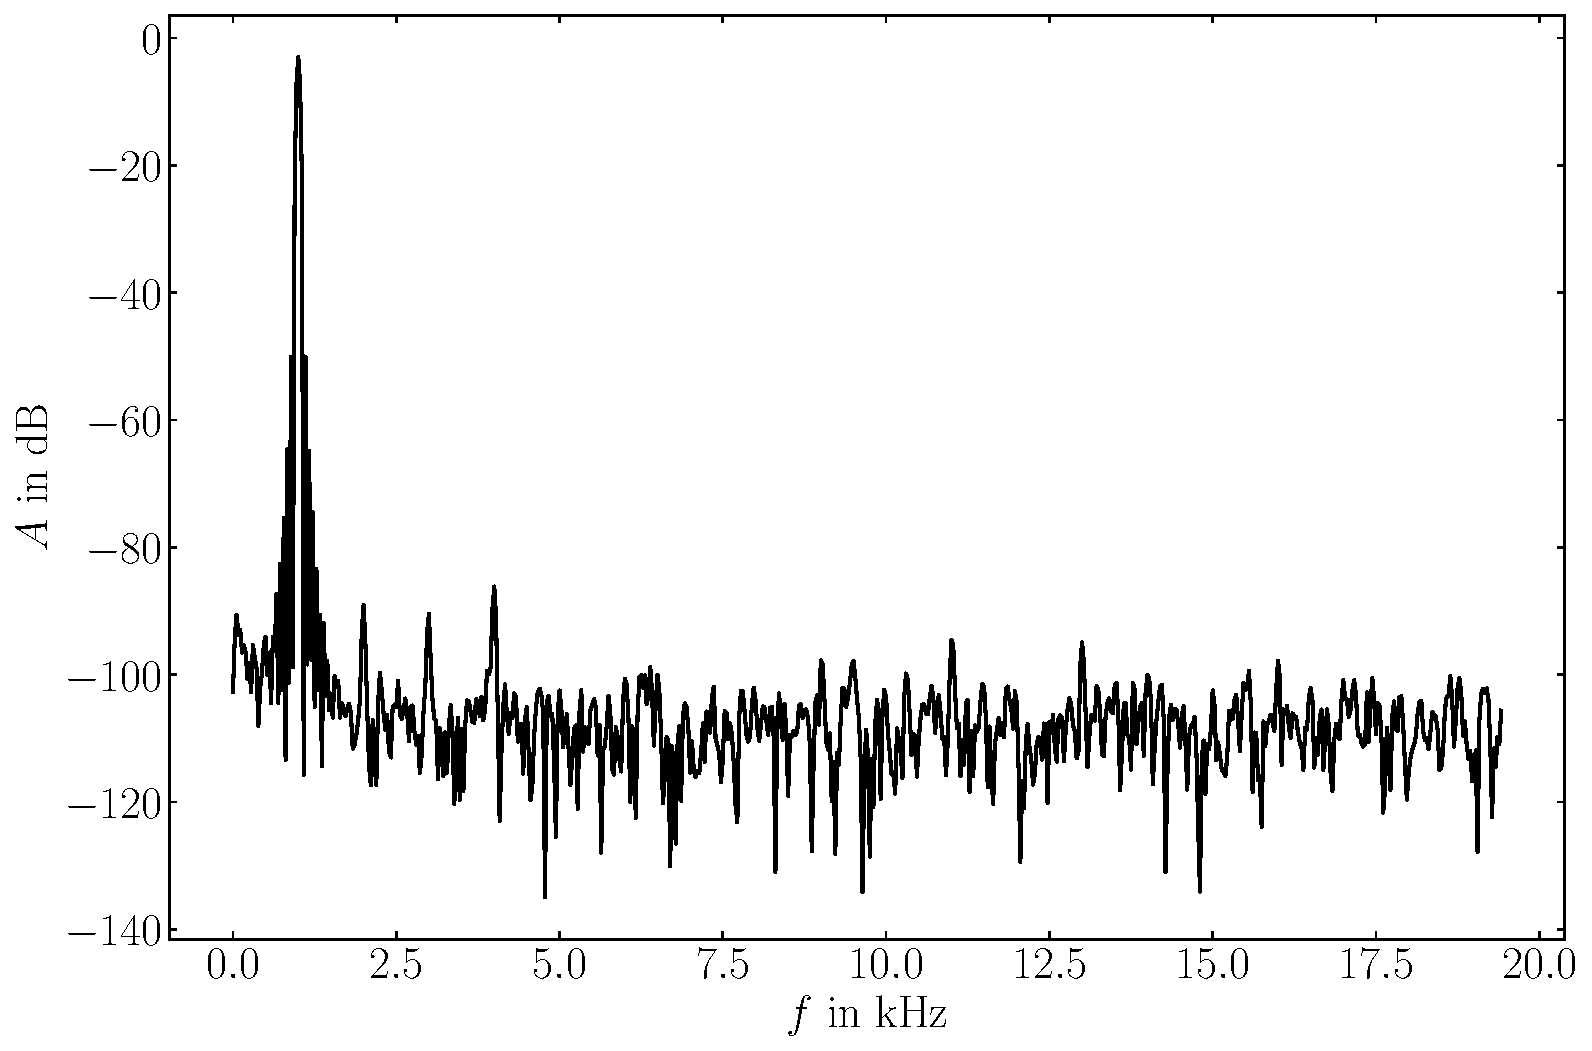
\includegraphics[scale = 0.5]{Manuel/41/FourierSinus.pdf}
    \captionof{figure}{Fourierspektrum der Sinusschwingung}
    \label{image:fourierSinus}
\end{center}
Wie in Abbildung \ref{image:fourierSinus} zu sehen, ist ein deutlich ausgeprägter Peak bei einer Frequenz von 1\,kHz zu erkennen. Nach Kapitel \ref{sec:fourierseries} sollte aber das Fourierspektrum nur einen Peak in Form einer Delta-Funktion bei der eingestellten Frequenz besitzen. Dies ist in der realen Welt aufgrund von Rauschen nicht möglich, wodurch der Hauptpeak bei 1\,kHz als eine breite Delta-Funktion gemessen wird. Weiterhin ist in Abbildung \ref{image:fourierSinus} neben dem Hauptpeak deutlich noch weiter kleinere Peaks zu erkennen, welche selbst in einem Abstand von 1\,kHz auftreten. Diese Peaks werden durch die Umgebungseinflüsse aus Kapitel \ref{sec:umwelt} und durch die Netzspannungsquelle selbst verursacht.


\newpage
\paragraph{c)}\textbf{Einfluss Mittelung auf Rechteckschwingung}

Nun wird der Einfluss der Anzahl der Mittelung $N$ auf eine Rechteckschwingung mit einer Amplitude $U_0=$ 1\,V mit einem Rauschen der Bandbreite $f_{Band}=$ 20\,MHz und einer AM Depth $=$ 120\,\% betrachtet.
In Abbildung \ref{image:einflussMittelung} ist zu erkennen, dass sich mit der Zunahme der Anzahl der Mittelungen $N$ der Signal/Rausch-Abstand $d$ zunimmt. Dies war zu erwarten, da schon wie in Kapitel \ref{sub:mittelung} erklärt, bei der Mittelung das Signal des Rauschens nur um den Faktor $\sqrt{N}$ zunimmt, während das Signal der Rechteckschwingung proportional zur Wiederholung anwächst. Um diesen Umstand graphisch darzustellen werden zuerst die Peaks der Rechteckschwingung und der Median bei jeder Mittelung mit einem Python-Skript bestimmt. Der Median jeder Mittelung ist in Abbildung \ref{image:mittelung} als \textit{gestrichelte Linie} in zugehöriger Farbe mit eingezeichnet. Der Signal/Rausch-Abstand $d$ wird dann mit der folgenden Formel bestimmt:
\begin{gather}
    d = \abs{\text{Median} - \text{Maxima}}
\end{gather}
Als Maxima wird der Wert des ersten Peaks verwendet, welcher -6.91\,dB beträgt. Die Berechnung ergibt dann folgende Tabelle:
\begin{center}
    \begin{tabular}{l | c}
        $N$ & $d$/dB\\
        \hline
        0   & 60,28 \\
        10  & 70,61 \\
        50  & 77,65 \\
        100 & 80,39 \\
    \end{tabular}
\end{center}
Da die Werte in dB angegeben sind, muss die Fit-Funktion logaritmisch sein. Der Fit wird mit dem Modul curve\_fit aus dem scipy.optimize Paket erstellt. Die Funktion hat dabei die Form:
\begin{gather}
    \begin{aligned}
       %&d(N) = a\cdot\sqrt{N} + t &\xrightarrow{\text{Fit}} &~~d(N) = 1.99\,\text{dB}\cdot\sqrt{N} + 62.17\,\text{dB} \\
       &d(N) = a\cdot\ln(\sqrt{N+1}) + t &\xrightarrow{\text{Fit}} &~~d(N) = 8,77\,\text{dB}\cdot\ln(\sqrt{N+1}) + 60.24\,\text{dB} \\
    \end{aligned}
\end{gather}
In Abbildung \ref{image:abstandMittelung} erkennt man deutlich, dass der Fit mit der Theorie gut übereinstimmt, was diese wiederum bestätigt. Womit sich sagen lässt, dass sich der Signal/Rausch-Abstand $d$ mit zunehmender Mittelung $N$ vergrößert und es somit möglich ist, das Signal besser aufzulösen.
%In Abbildung \ref{image:abstandMittelung} erkennt man deutlich, dass die natürliche Logarithmus-Funktion besser den Verlauf der Datenpunkten entspricht als die theoretisch erwartete Wurzel-Funktion. Dies kann mit der Wahl der Berechnung des Signal/Rausch-Abstands zusammenhängen. Dennoch lässt sich sagen, dass sich der Signal/Rausch-Abstand $d$ mit zunehmender Mittelung $N$ vergrößert und es somit möglich ist, das Signal besser aufzulösen.
\newpage
\begin{center}
    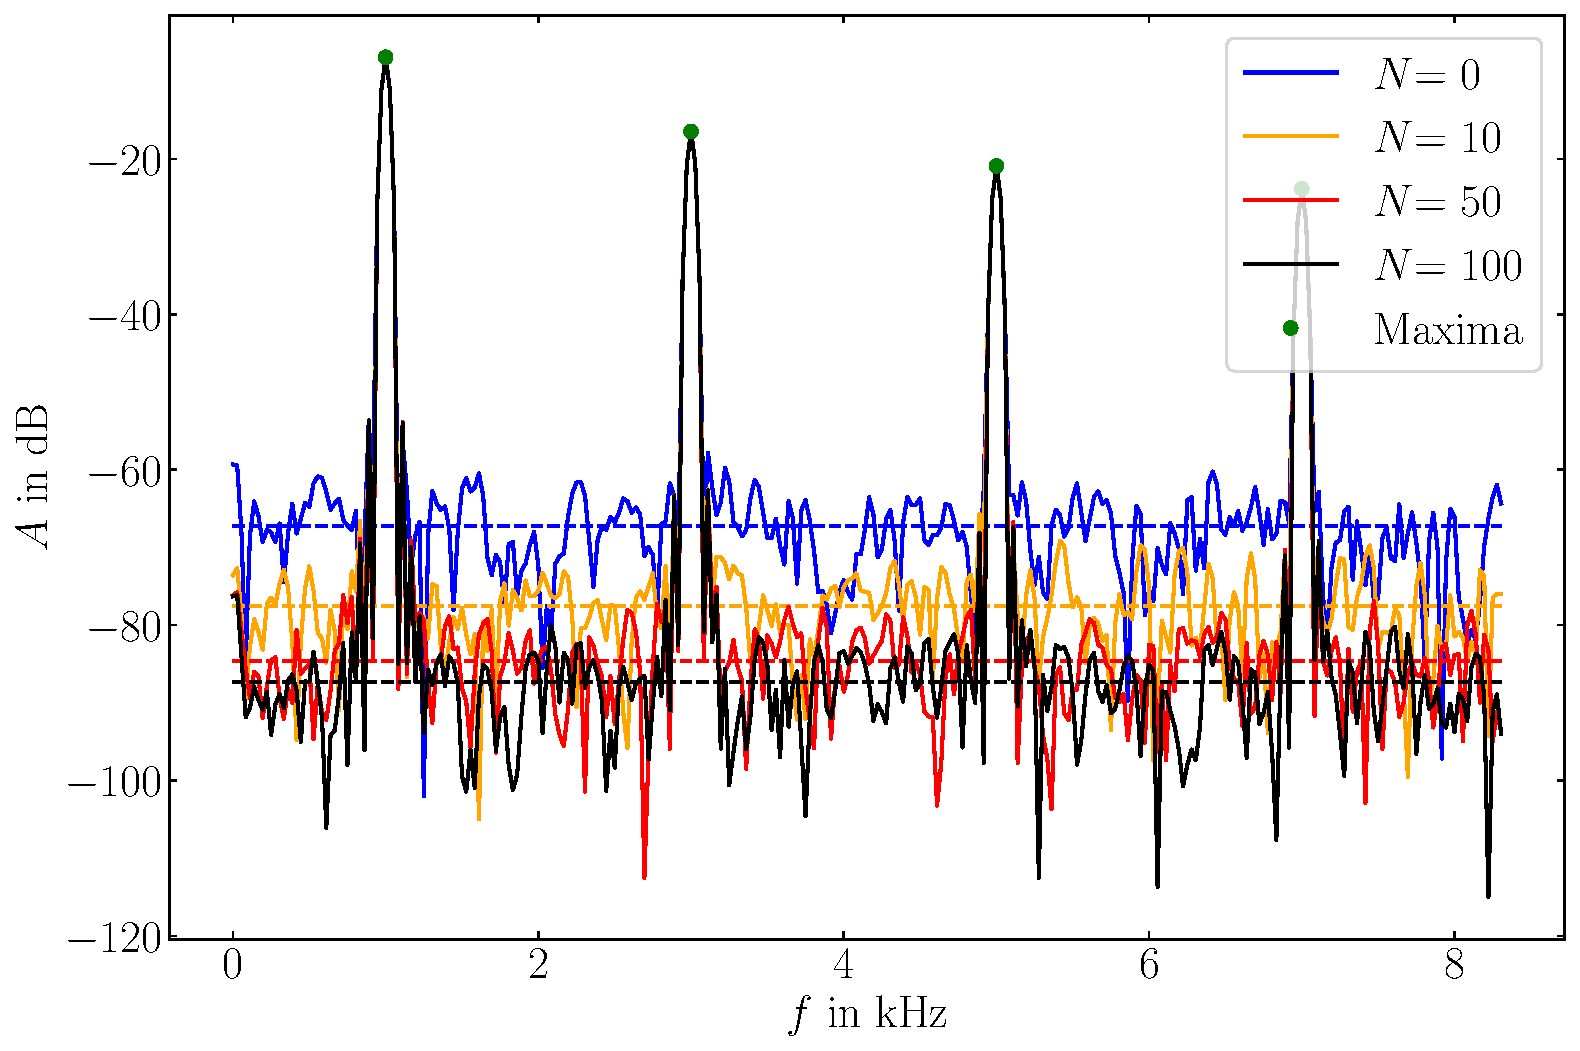
\includegraphics[scale = 0.5]{Manuel/41/Mittelung.pdf}
    \captionof{figure}{Einfluss der Mittelung auf Fourierspektrum einer Rechteckschwingung}
    \label{image:einflussMittelung}
\end{center}
\begin{center}
    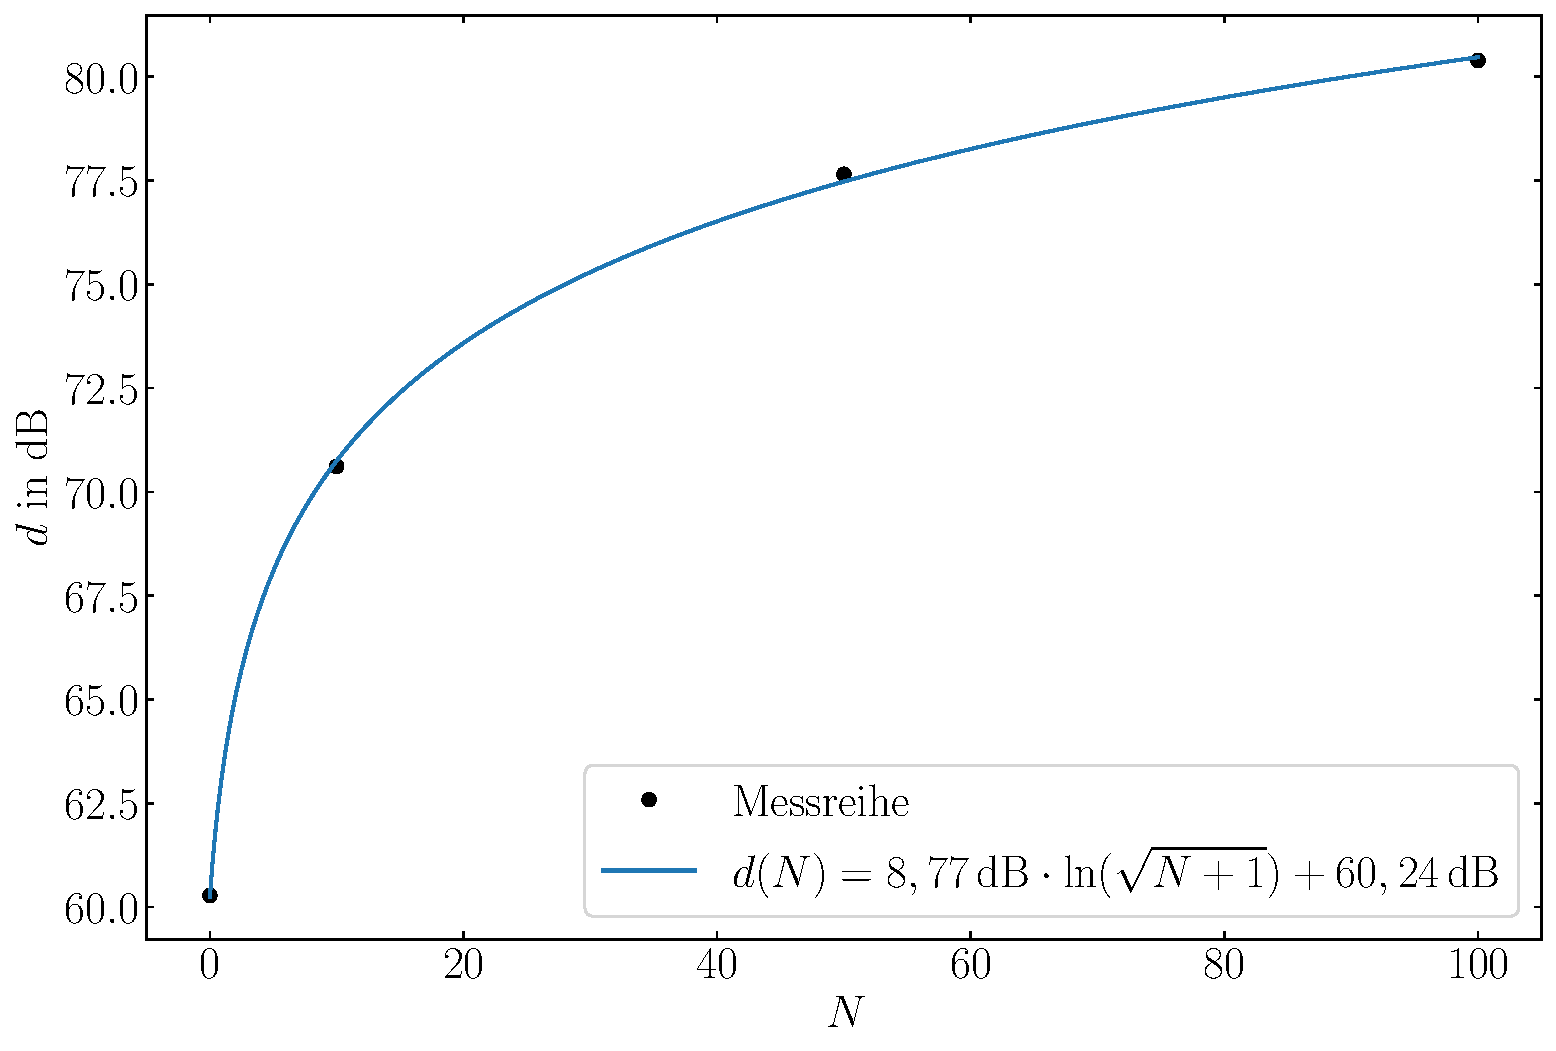
\includegraphics[scale = 0.5]{Manuel/41/MittlungAbstand.pdf}
    \captionof{figure}{Signal-Rausch Abstand in Abhängigkeit der Mittelungen $N$}
    \label{image:abstandMittelung}
\end{center}

\newpage
\paragraph{d)}\textbf{Einfluss Signal/Rausch-Abstand auf zeitliche Signalform}

Als weiteres wird der Einfluss des Signal/Rausch-Verhältnis $V_{SR}$ auf die Signalform einer Rechteckschwingung mit einer Amplitude $U_0=$ 1\,V und einen Bandbreite\\$f_{Band}=$ 20\,MHz betrachtet.
In Abbildung \ref{image:sigRauRechtAll} ist zuerst der Einfluss des Signal/Rausch-Abstands auf die komplette Rechteckschwingung dargestellt. Schon hier erkennt man, dass mit höherem Signal/Rausch-Verhältnis das \enquote{Ausschlagen} der Amplitude des Rauschens zunimmt. Noch deutlich ist dies im Ausschnitt des oberen Umkehrpunkts der Rechteckschwingung in Abbildung \ref{image:sigRauRechtAll} zu erkennen. Dies bedeutet, dass für kleine $V_{SR}$ das Verhältnis aus Nutzsignal und Störsignal (Rauschen) abnimmt, aber der Signal/Rausch-Abstand $d$ zunimmt und somit das Rauschen weniger Anteil am eigentlichen Signal hat. Die Änderung des Signal/Rausch-Verhältnis $V_{SR}$ hat aber keinen generellen Einfluss auf den Verlauf der Signalform der Rechteckschwingung. 
\begin{center}
    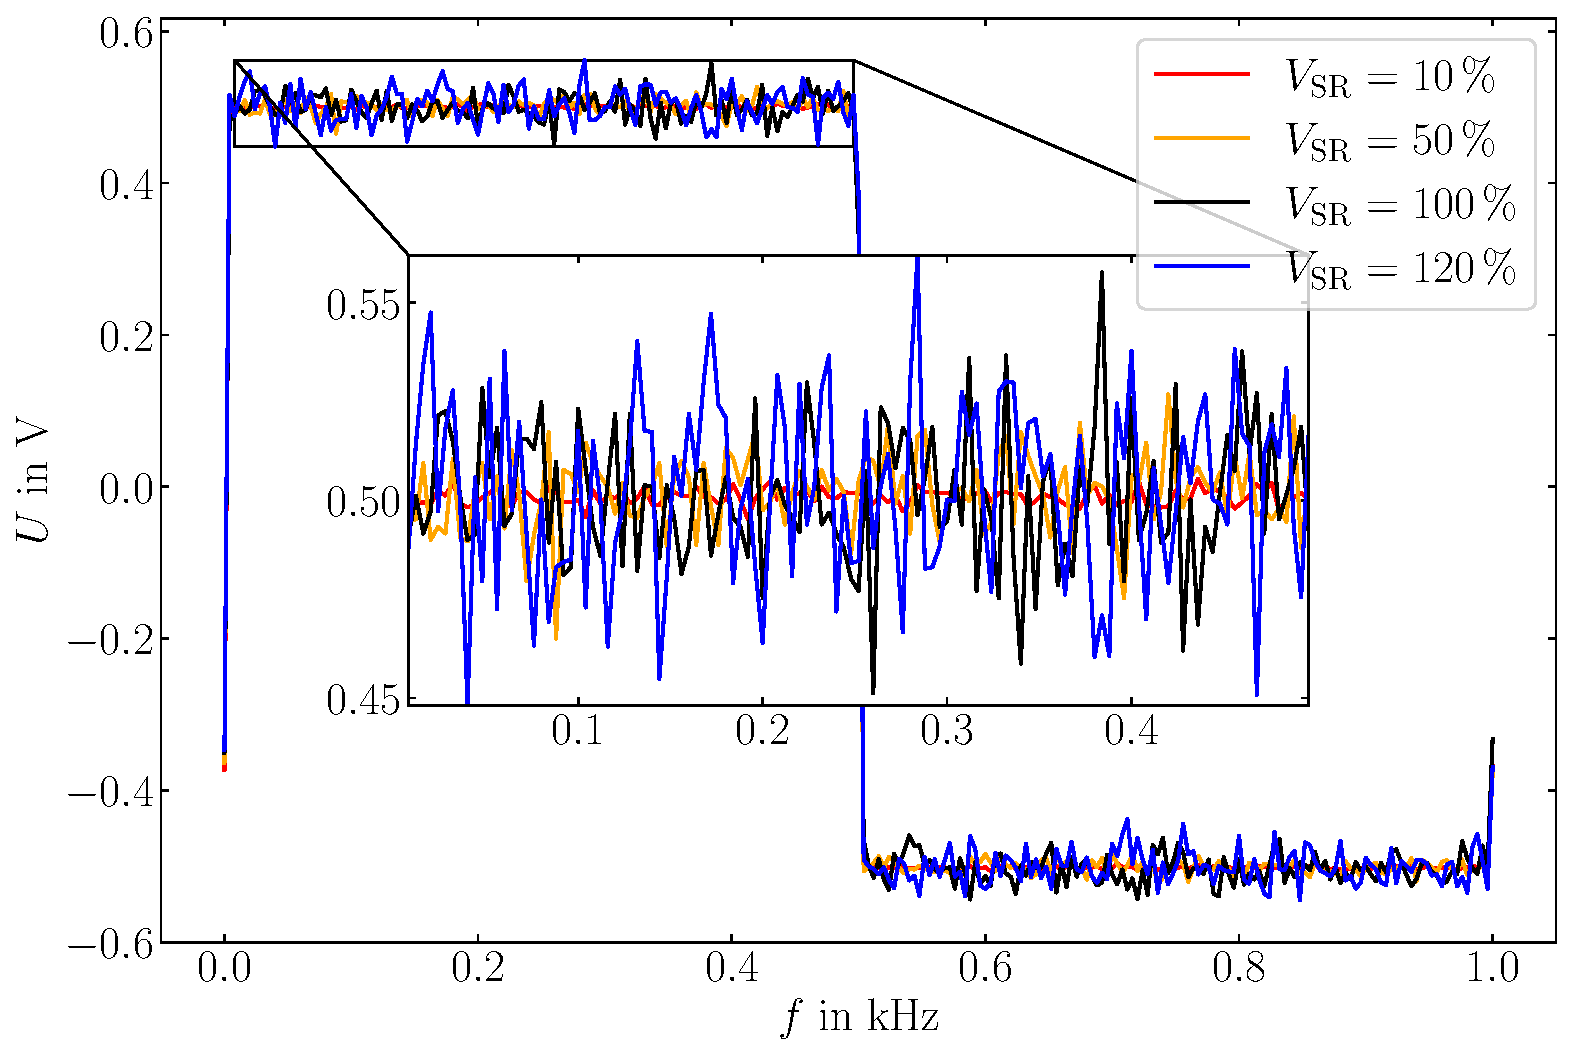
\includegraphics[scale = 0.5]{Manuel/41/SignalRauschAbstandAll.pdf}
    \captionof{figure}{Einfluss Signal/Rausch-Abstand mit Ausschnitt vom obere Umkehrpunkt der Rechteckschwingung}
    \label{image:sigRauRechtAll}
\end{center}
\newpage
%\begin{center}
%    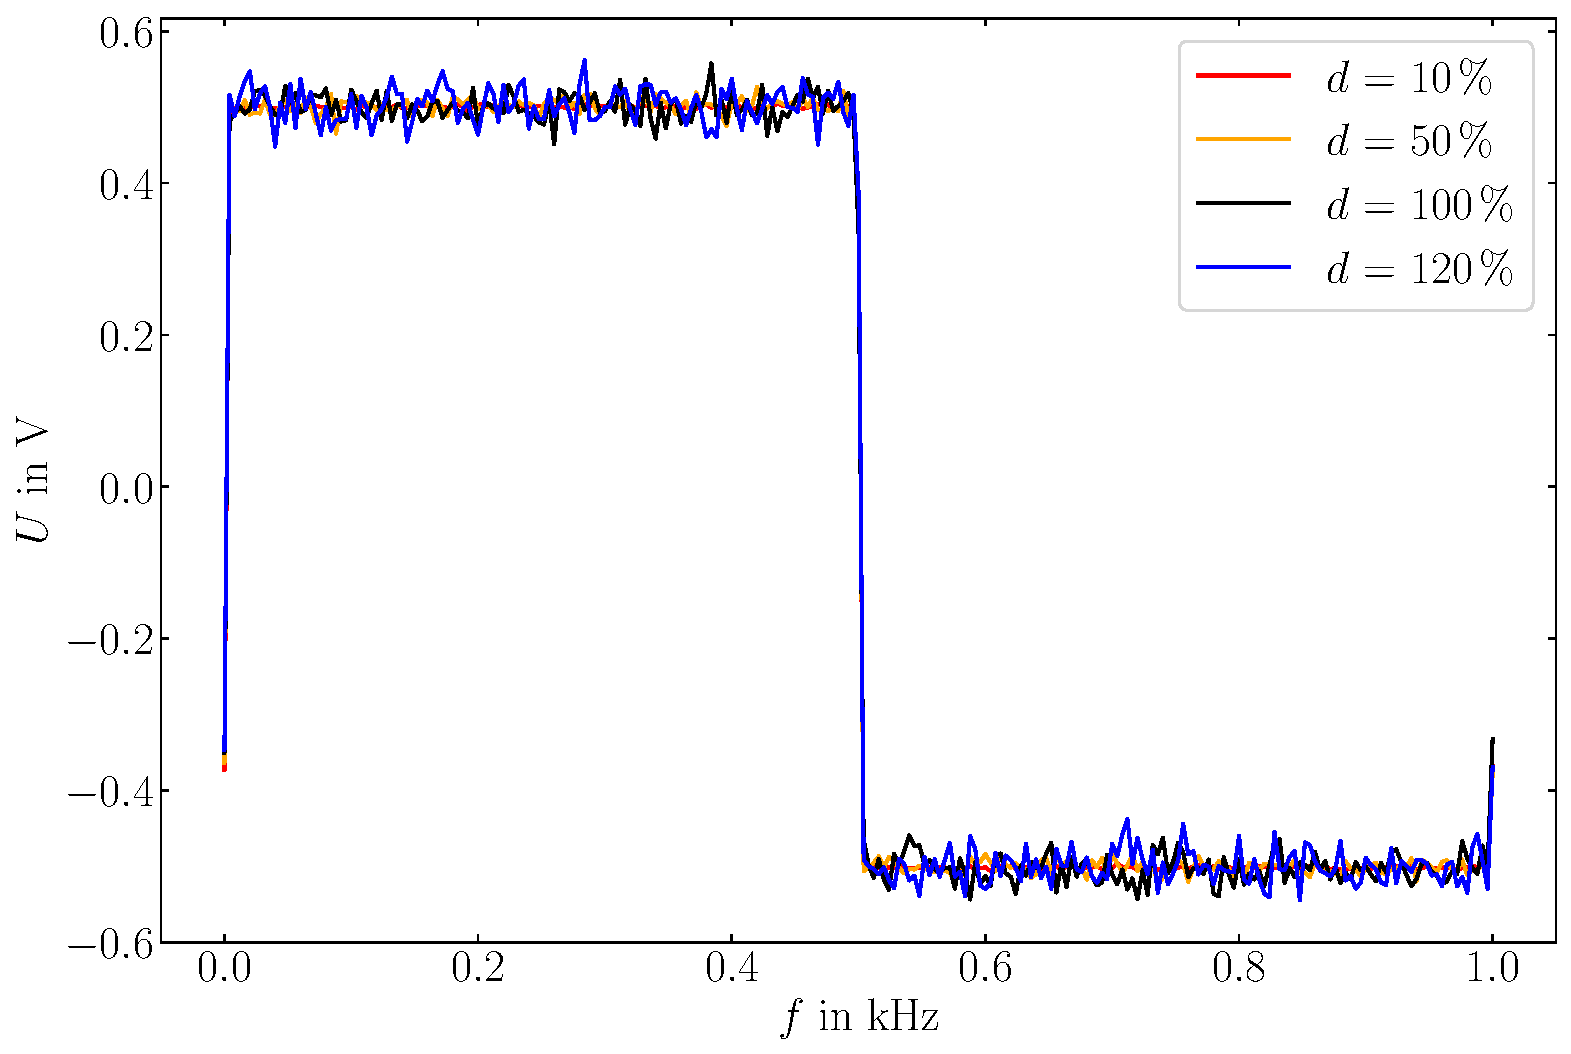
\includegraphics[scale = 0.5]{Manuel/41/SignalRauschAbstandKomplett.pdf}
%    \captionof{figure}{Einfluss Signal/Rausch-Abstand auf komplette Rechteckschwingung}
%    \label{image:sigRauRechtKomplett}
%\end{center}
%\begin{center}
%    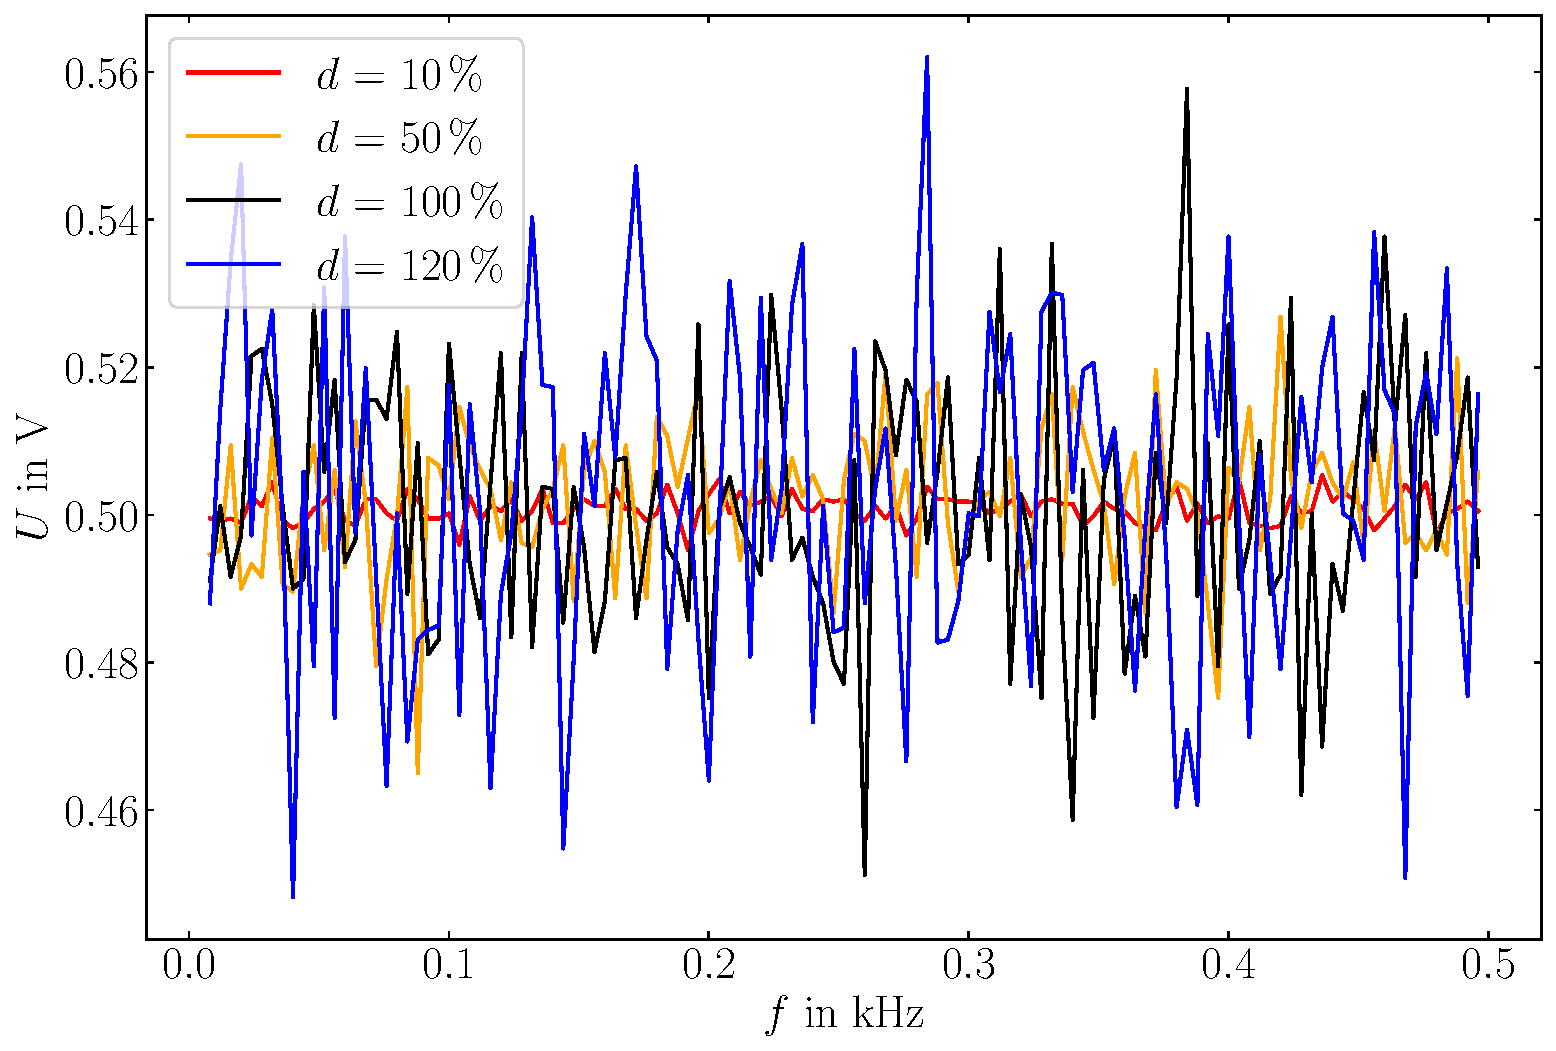
\includegraphics[scale = 0.5]{Manuel/41/SignalRauschAbstand.pdf}
%    \captionof{figure}{Einfluss Signal/Rausch-Abstand im Ausschnitt vom obere Umkehrpunkt der Rechteckschwingung}
%    \label{image:sigRauRecht}
%\end{center}


\paragraph{e)}\textbf{Einfluss Bandbreite auf zeitliche Signalform}

Zuletzt in diesem Kapitel wird der Einfluss der Bandbreite auf die zeitliche Signalform besprochen. Dabei wird wieder eine Rechteckschwingung mit einer Amplitude\\ $U_0=$ 1\,V und einem Signal/Rausch-Abstand $d=$ 100\,\% verwendet. In Abbildung \ref{image:bandbreiteRechtKomplett} wird erneut eine komplette Rechteckschwingung gezeigt. Darauf erkennt man, dass der Funktionsgenerator die Form des Rechtecksignals mit kleineren Bandbreiten $f_{Band}$ nicht mehr erzeugen kann. Vor allem bei Frequenzen unter 100\,kHz. Aber auch eine Zunahme des Rauschens ist zu erkennen, wenn die Bandbreite kontinuierlich abnimmt. Dies bestätigt auch das Fourierspektrum (Abb. \ref{image:bandbreiteRechtFourier}). Darin ist eine Zunahme des Signal/Rausch-Abstands $d$ zu erkennen, was bedeutet, dass bei höheren Bandbreiten das Rauschen auf dem Rechtecksignal abnimmt. In Abbildung \ref{image:bandbreiteRecht} kann man dies noch genauer betrachten.
\begin{center}
    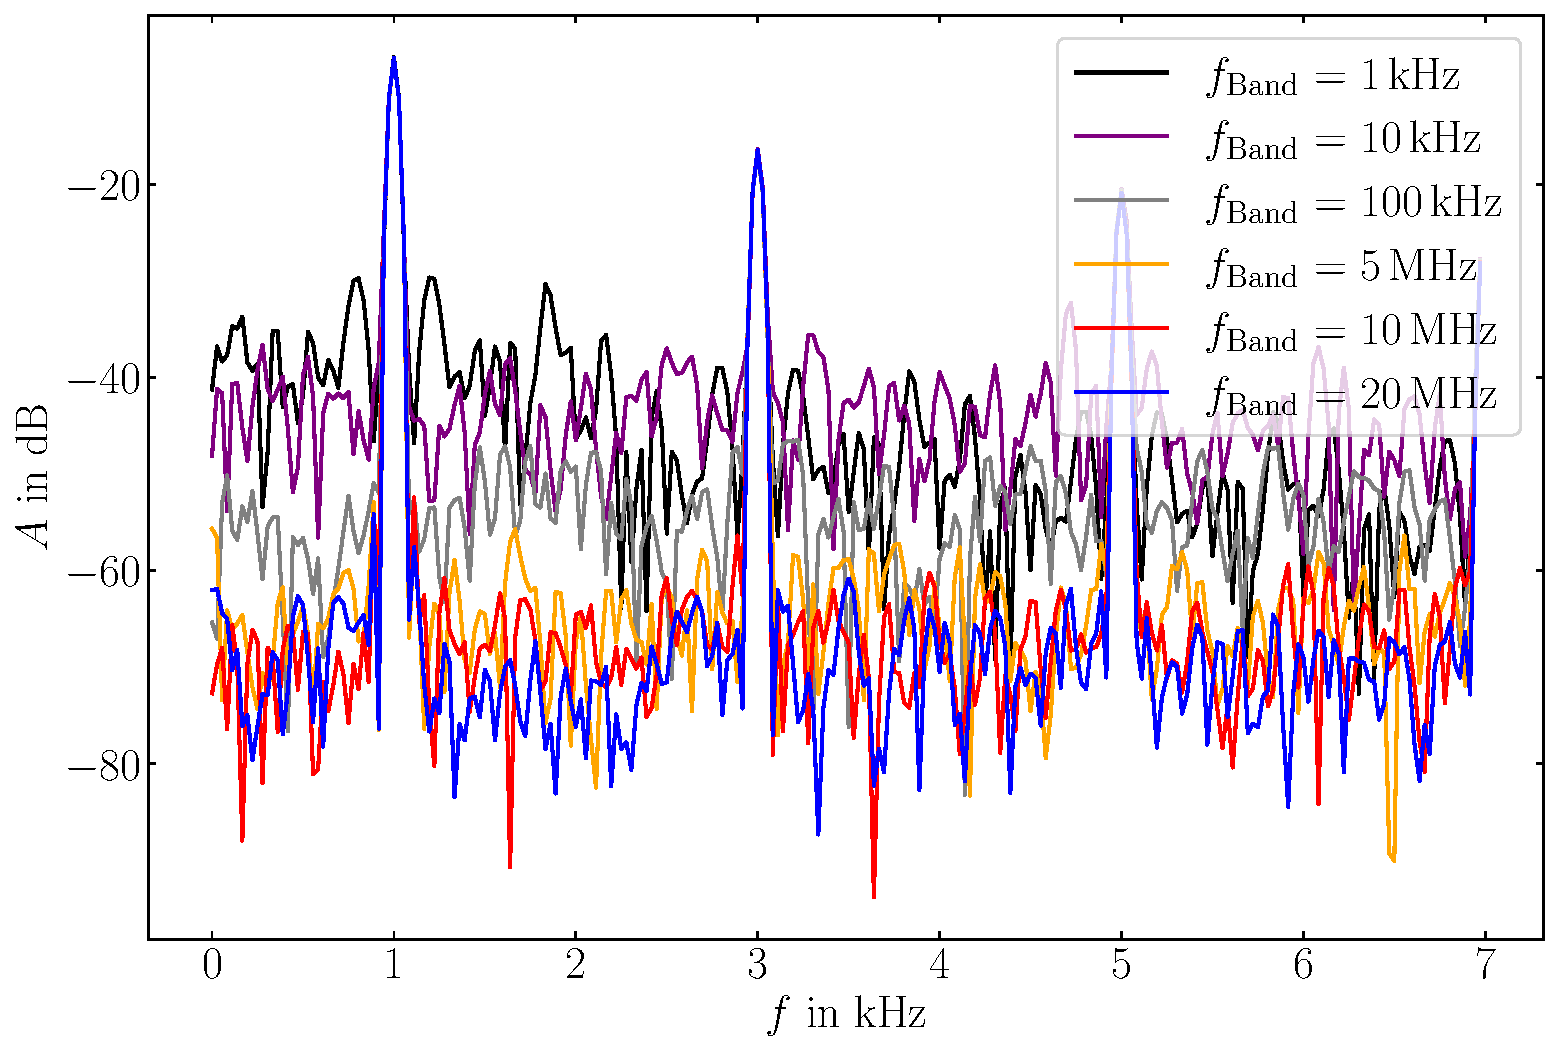
\includegraphics[scale = 0.5]{Manuel/41/BandbreiteFourier.pdf}
    \captionof{figure}{Einfluss Bandbreite auf Rechteckschwingung im Fourierspektrum}
    \label{image:bandbreiteRechtFourier}
\end{center} 
\newpage
\begin{center}
    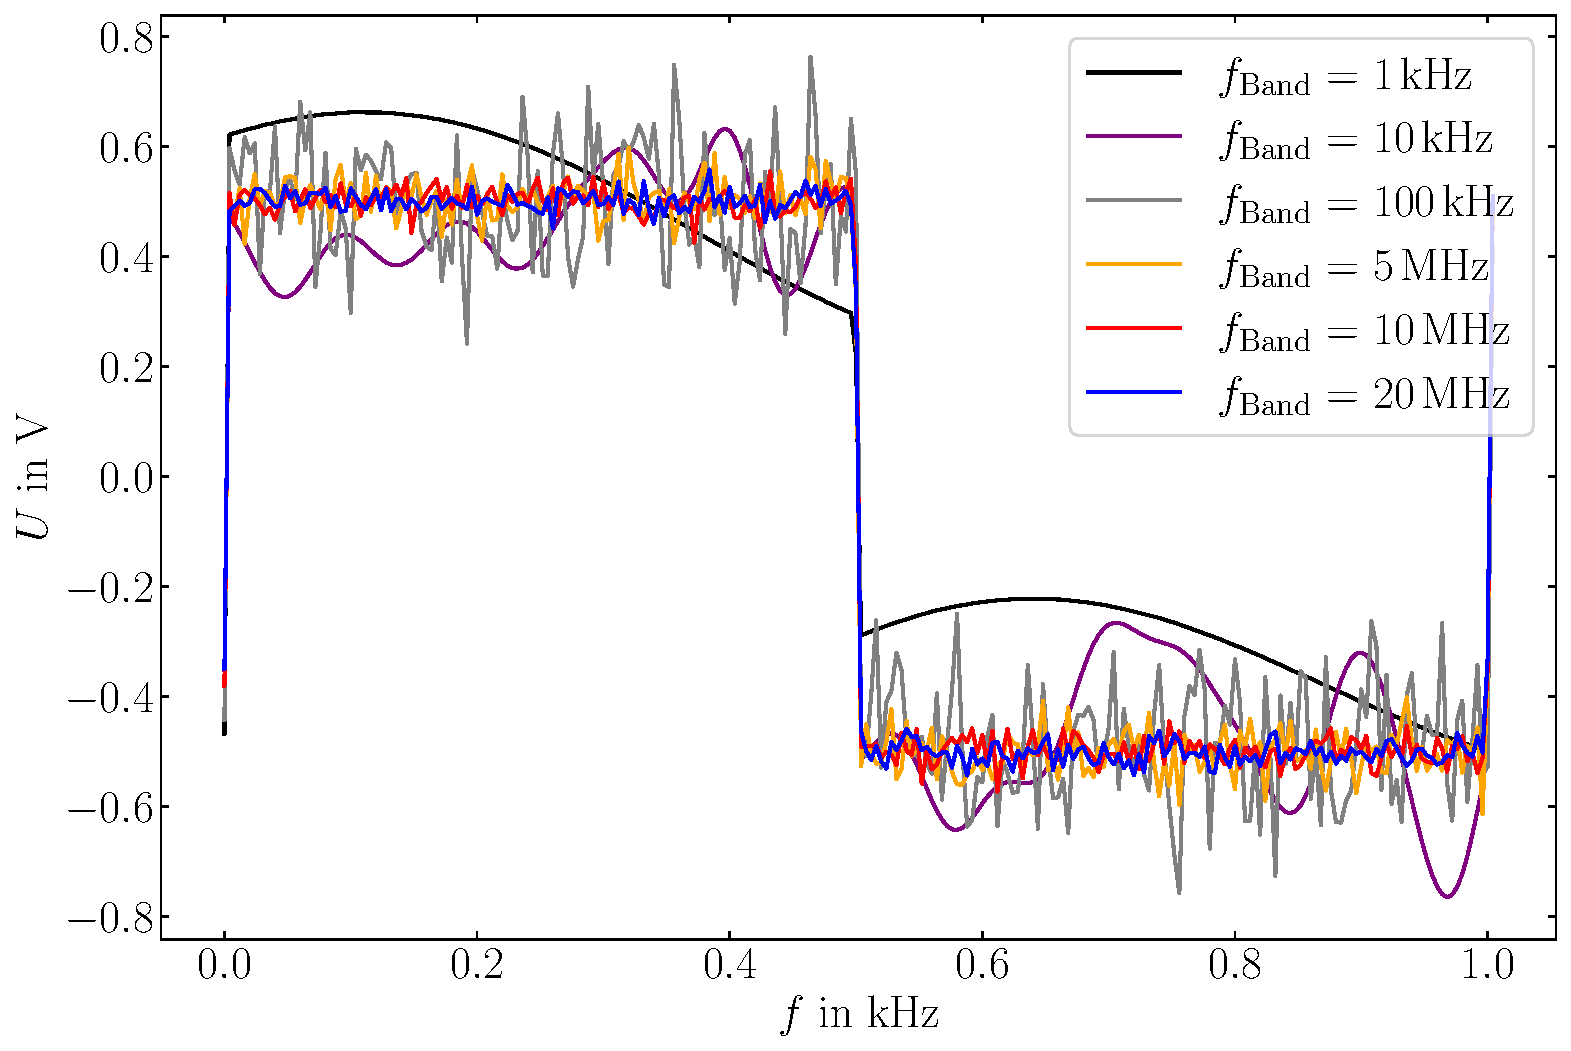
\includegraphics[scale = 0.5]{Manuel/41/BandbreiteKomplett.pdf}
    \captionof{figure}{Einfluss Bandbreite auf komplette Rechteckschwingung}
    \label{image:bandbreiteRechtKomplett}
\end{center}
\begin{center}
    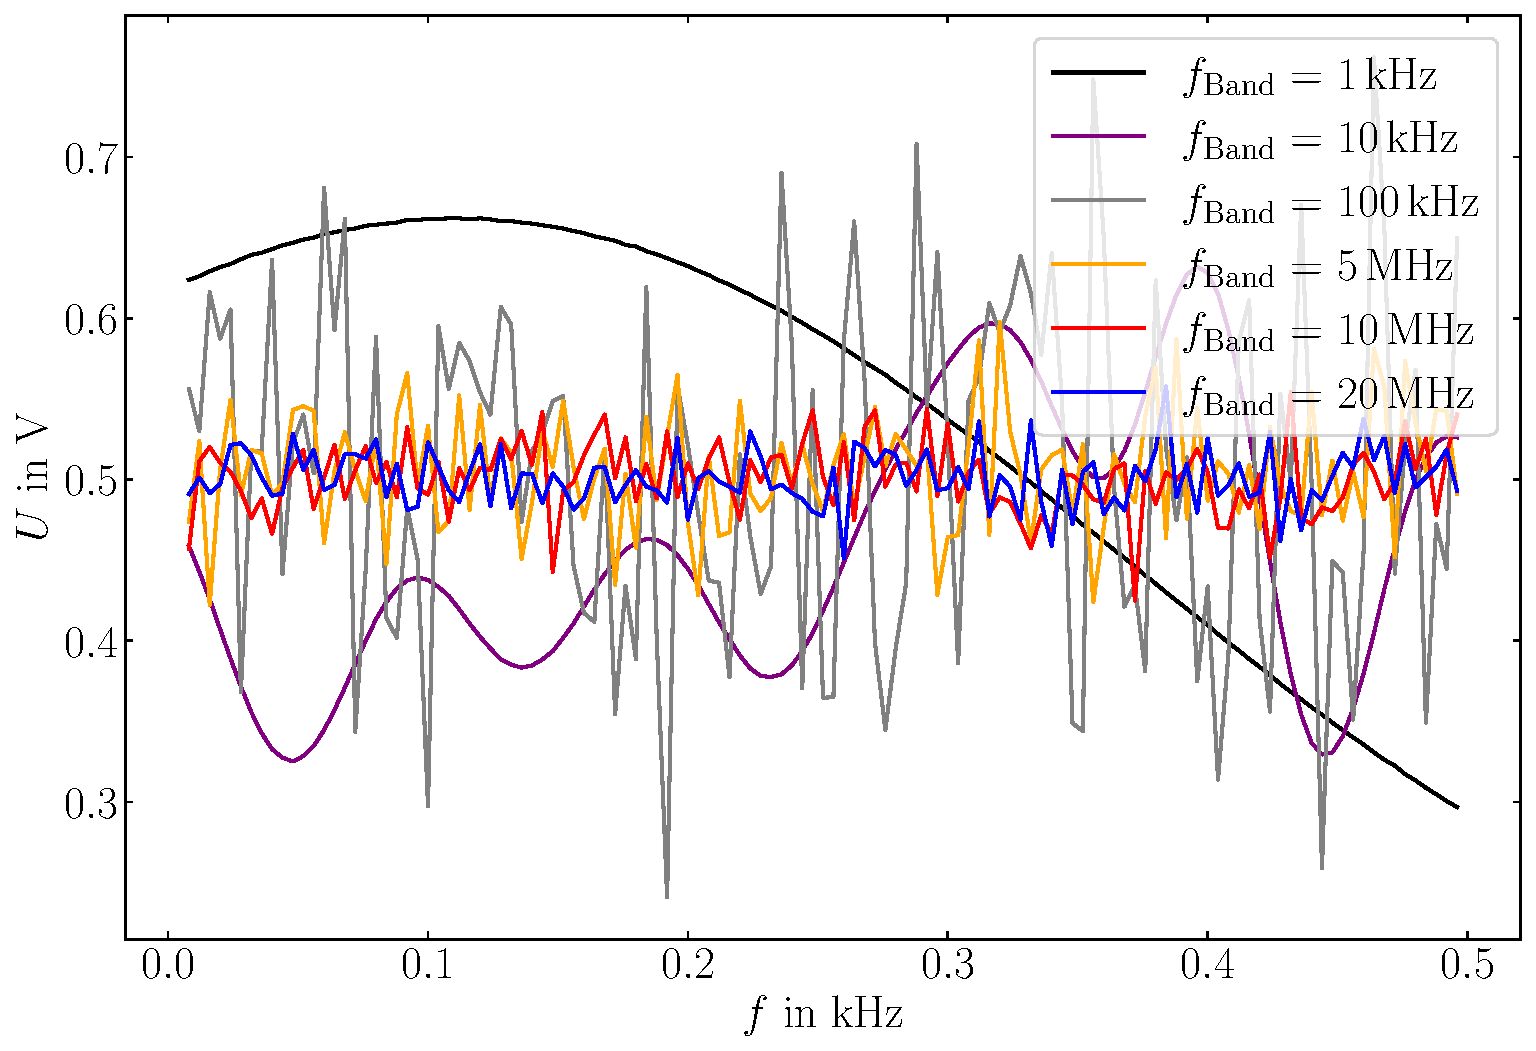
\includegraphics[scale = 0.5]{Manuel/41/Bandbreite.pdf}
    \captionof{figure}{Einfluss Bandbreite im Ausschnitt vom obere Umkehrpunkt der Rechteckschwingung}
    \label{image:bandbreiteRecht}
\end{center} 


\newpage
\section{Theorem von Nyquist}

Im Folgenden soll das Theorem von Nyquist genauer betrachtet werden. Dafür wird der Ausgang des Frequenzgenerator direkt mit dem Eingang des Messcomputers verbunden, parallel dazu wird der Ausgang des Generators mit dem Osziloskop überprüft.\\
Das Theorem besagt das ein Signal, begrenzt mit $f_{max}$, nur mit einer Abtastfrequenz von größer $f_{crit}$ exakt rekonstruiert werden kann.
\begin{align}
    f_{crit} = 2 \cdot f_{max}
\end{align}


Um dies genauer zu untersuchen wurde zuerst die Abtastrate für ein unverrauschtes Sinussignal ($f = 20$\,kHz) variiert und gegen die gemessene Frequenz aufgetragen.
\begin{figure}[h]
    \centering
    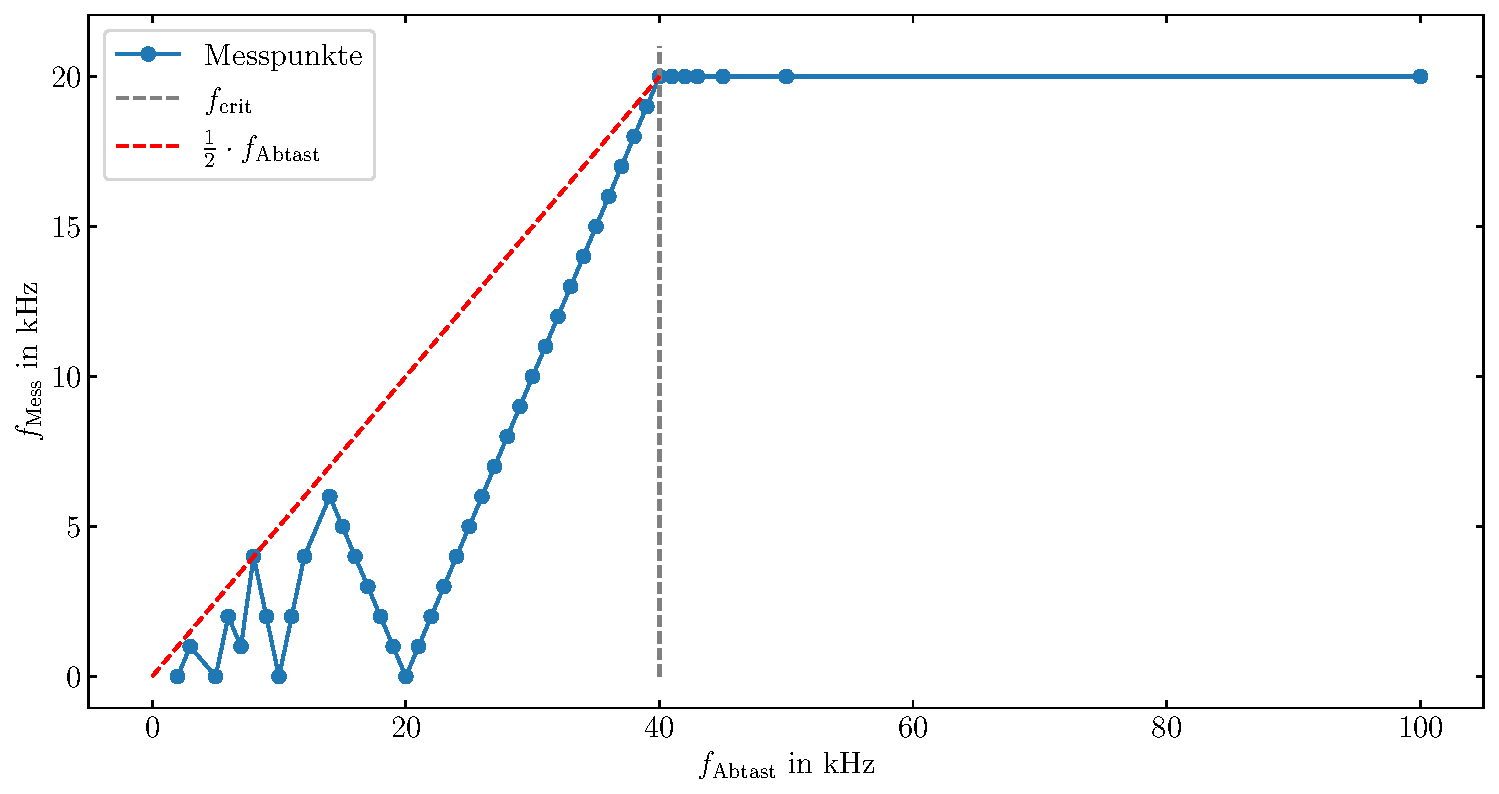
\includegraphics[width=\textwidth]{Paul/42a1.pdf}
    \caption{Variation der Abtastrate gegen die gemessene Frequenz, bei konstanter Generatorfrequenz von 20 kHz.}
    \label{fig:42a1}
\end{figure}

In Abbildung \ref{fig:42a1} ist deutlich zu erkennen, dass für die Abtastfrequenz $f_{Abtast} > f_{crit}$ die Frequenz korrekt gemessen wird. Bei unterschreiten der kritischen Frequenz fällt die gemessene Frequenz jedoch unter den eigentlichen Wert, bis $f = f_{Abtast}$. Wenn die Abtastfrequenz gleich der Generatorfrequenz ist, wird eine Frequenz von 0 Hz gemessen, also ein konstantes Signal. Das ist logisch, da der Detektor immer den gleichen Punkt der Signalabfolge misst und dies somit als konstantes Signal wahrnimmt. Dies tritt nicht nur für $f = f_{Abtast}$ auf, sondern immer dann wenn $f_{Abtast} = n \cdot f$ mit $ n= 1,2,3...$. Aus diesem Grund entsteht vor der kritischen Frequenz ein sägezahnähnliches Muster.

\newpage
In der zweiten Messreihe wurde nun die Abtastrate ($f_{Abtast} = 20$\,kHz) konstant gehalten und die Frequenz des Generators wurde variiert, welche wiederum gegen die gemessene Frequenz aufgetragen wurde. Für die kritische Frequenz gilt nun:
\begin{align}
    f_{crit} = \frac{1}{2} f_{Abtast}
\end{align}
\begin{figure}[h]
    \centering
    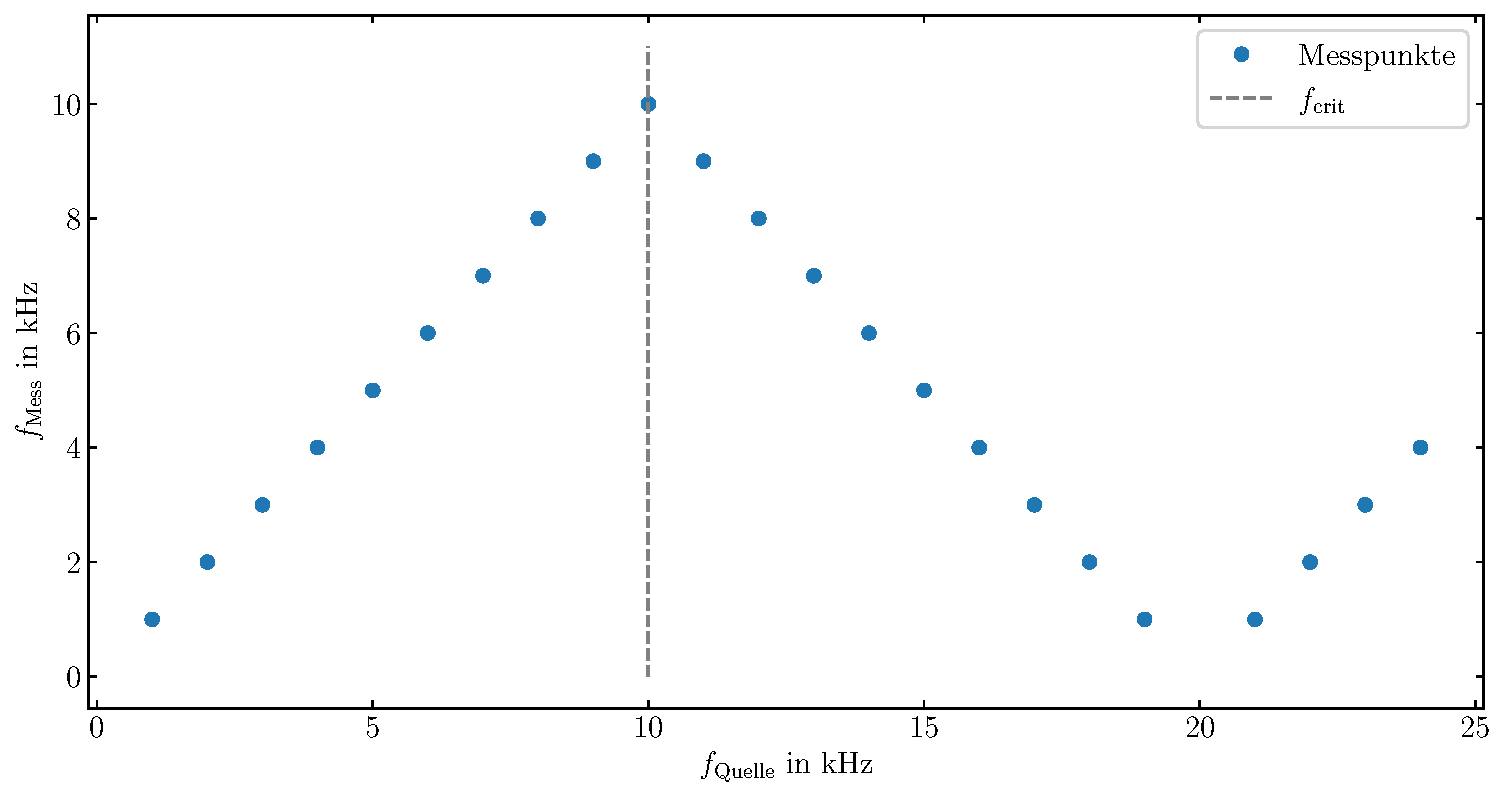
\includegraphics[width=\textwidth]{Paul/42a2.pdf}
    \caption{Variation der Generatorfrequenz gegen die gemessene Frequenz, bei konstanter Abtastfrequenz.}
    \label{fig:42a2}
\end{figure}
In Abbildung \ref{fig:42a2} ist wieder deutlich zu sehen, dass für $f_{Quelle} < f_{crit}$ die Frequenz richtig gemessen wird. Ist dies jedoch nicht mehr der Fall, so tritt analog zu oben wieder ein Sägezahnmuster auf.


\newpage
Des Weiteren wurde das Fourierspektrum eines Dreieckssignal ($f = 3$\,kHz), mit einer Abtastfrequenz von $f_s = 7$\,kHz, aufgenommen.
\begin{figure}[h]
    \centering
    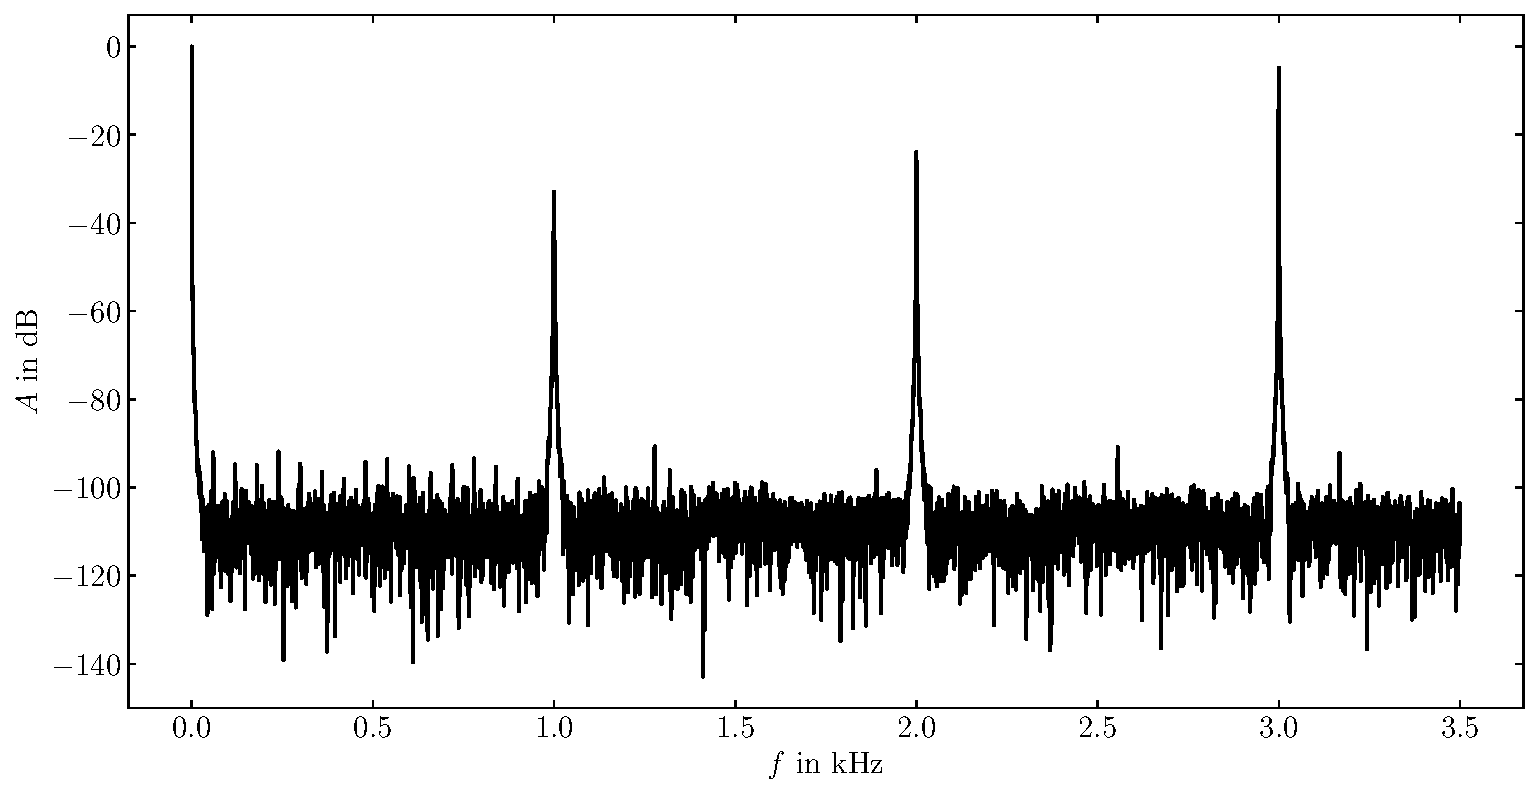
\includegraphics[width=\textwidth]{Paul/42b-fs7kHz.pdf}
    \caption{Fourierspektrum eines Dreieckssignal ($f = 3$\,kHz), $f_s = 7$\,kHz.}
    \label{fig:42a3}
\end{figure}

In Abbildung \ref{fig:42a3} ist der Effekt des Aliasing zu erkennen, das heißt der Detektor kann nicht unterscheiden, welche die richtig gemessene Frequenz ist und was die Aliase (falsche zugeordnete Messwerte) der eigentlichen Frequenz sind. Da die Generatorfrequenz bekannt ist, ist ebenfalls bekannt, dass die richtige Frequenz $f=3$\,kHz ist und die Peaks bei $f_1=1$\,kHz und $f_2=2$\,kHz die Aliase dieser sind. Hat man dieses wissen jedoch nicht, kann dies jedoch zu nicht unerheblichen Messfehlern führen. Um Aliasing zu vermeiden, sollte eine höhere Abtastfrequenz verwendet werden.\\

%TODO #42
Eine mögliche Erklärung für die Peaks bei 0kHz, 1kHz und 2kHz sind Umklappprozesse.
Umklappprozesse sind im allgemeinen Dreiphononenprozesse, für die Folgende Erhaltungssätze gelten:
\begin{align}
    \hbar \omega_1 +\hbar \omega_2 &= \hbar \omega_3  \qquad \text{Energierhaltung}\\
    \vec{q_1} + \vec{q_2} &= \vec{q_3} + \vec{G} \qquad \abs{\vec{G}} \neq 0 \label{eq:UPImp}
\end{align}
Gleichung \ref{eq:UPImp} lässt sich als Impulserhaltung auffassen, da \( \hbar \vec{q}\) der Quasiimpuls eines Phonons ist. Es handelt sich also um Stoßprozesse \citep{EFP}.\\
Die Erklärung für die Äquidistanz der Peaks hängt mit quantenmechanischen Effekten zusammen.
\newpage
\section{Signalfilterung}
In diesem Abschnitt soll die Signalfilterung genauer betrachtet werden. Dafür wird wieder der Ausgang des Generators mit dem Eingang des Analog-Digital-Wandlers verbunden. Parallel dazu wird der Ausgang des Generators mit dem Oszilloskop überwacht.

\subsection{Verschiedene Tiefpassfilterkurven}
\label{sec:VerTi}
Zuerst sollen die Filterkurven verschiedener Tiefpässe dargestellt werden. Hierzu wird am Generator ein Sinussignal ($f=100$\,Hz) mit einer Rauschbandbreite von 20\,MHz eingestellt.\\

%Für einen groben Überblick und um Unterschiede besser erkennen zu können werden alle Filterkurven in einem gemeinsamen Diagramm dargestellt (Abbildung \ref{fig:43aAll}). \\

\begin{center}
    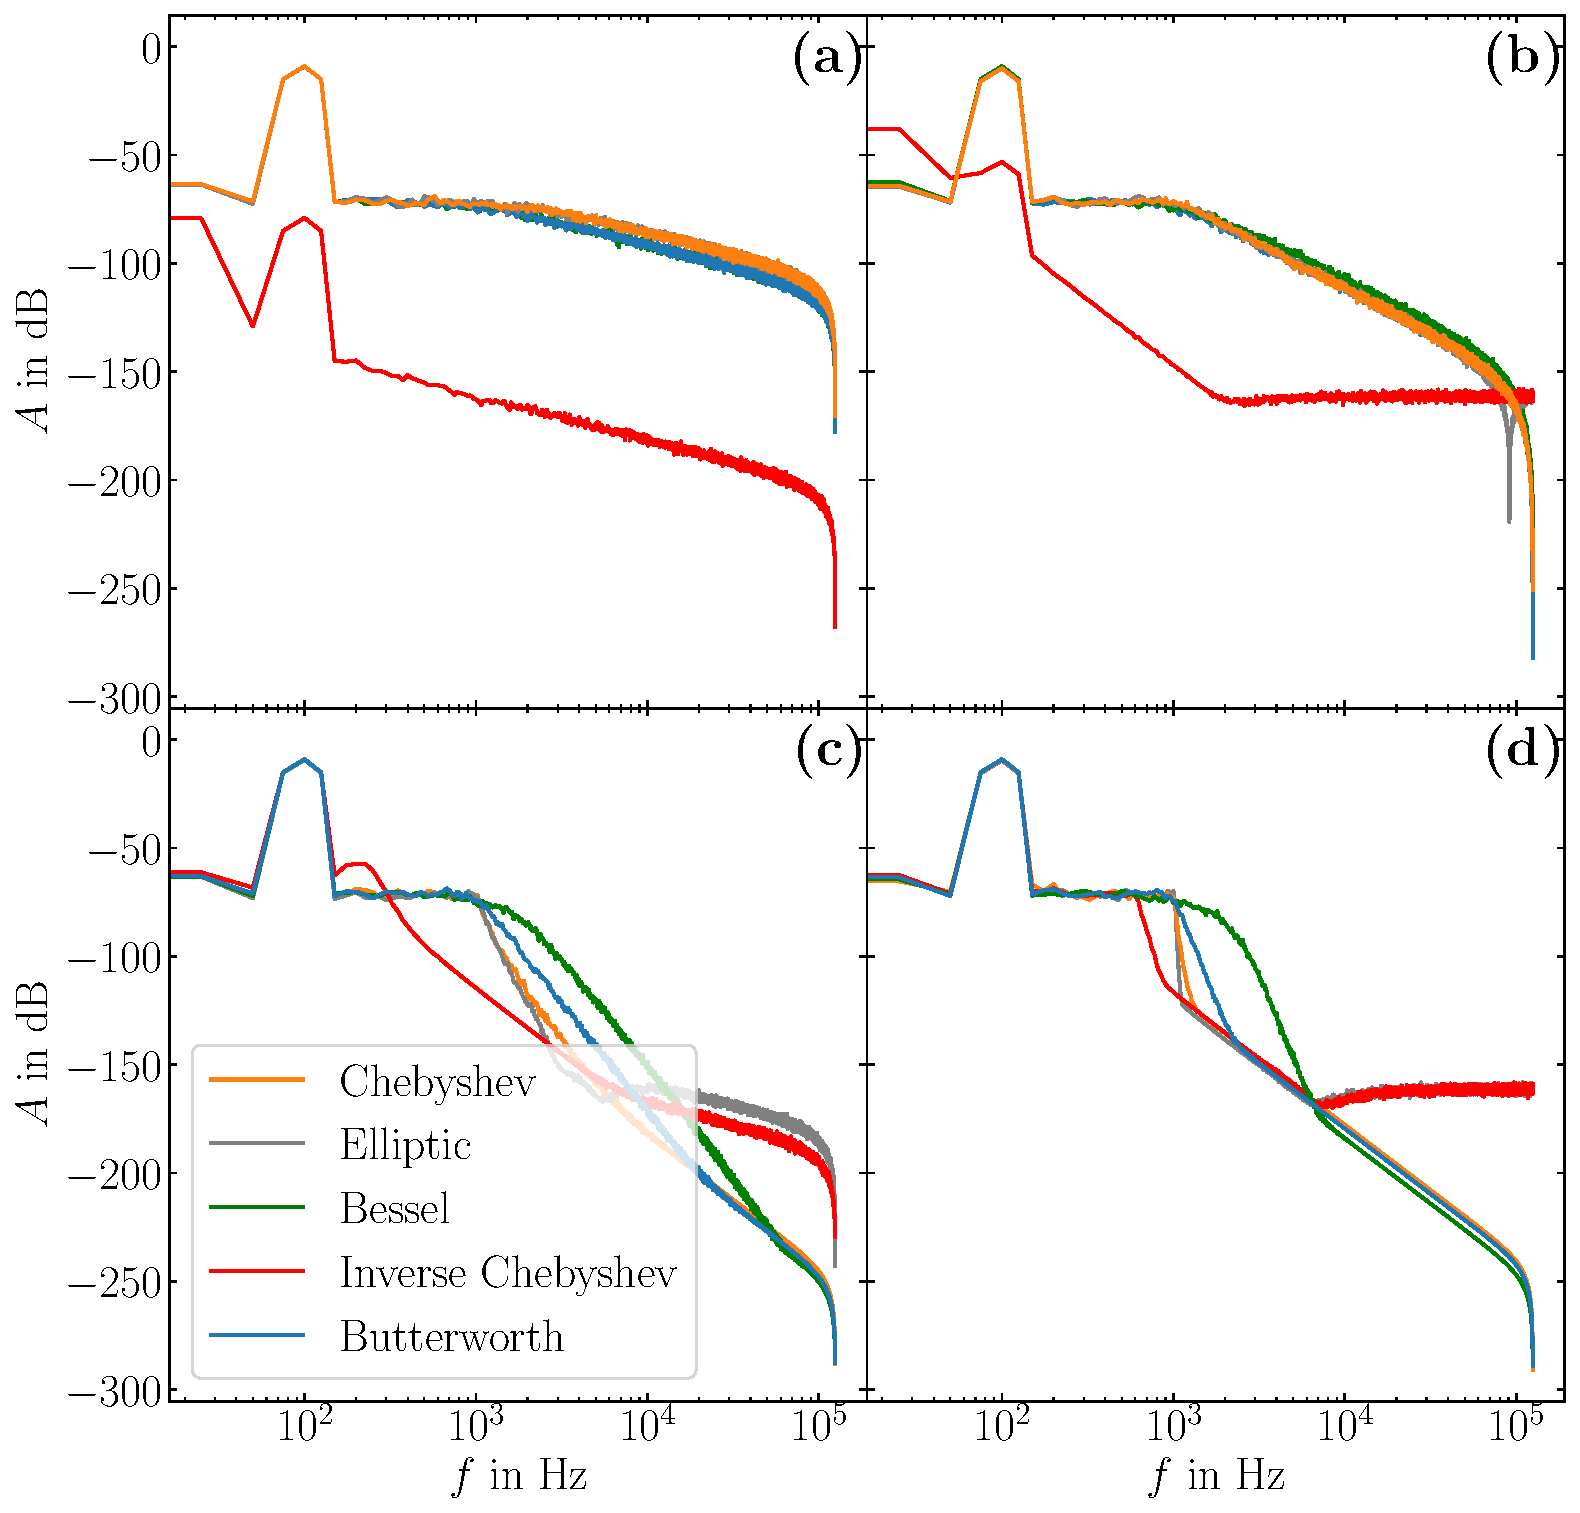
\includegraphics[width = 0.9\textwidth]{Paul/43aAllOrAll.pdf}
    \captionof{figure}{Fourierspektrum verschiedene Tiefpassfilter mit (a) Ordnung 1, (b) Ordnung 2, (c) Ordnung 5 und (d) Ordnung 10}
    \label{fig:43aAll}
\end{center}

In Abbildung \ref{fig:43aAll} fällt auf, dass sich Elliptic- und Chebyshevfilter fast deckungsgleich überlagern. Auch Butterworth- und Besselfilter sind fast deckungsgleich mit den oben genannten lediglich für Frequenzen zwischen ca. $1\cdot 10^3$\,Hz und $1\cdot 10^5$\,Hz divergieren sie geringfügig. Am stärksten weicht der inverse Chebyshevfilter von den anderen ab. Der Verlauf ist sehr ähnlich, nahezu parallel, jedoch ist sie Kurve nach unten verschoben. Für höhere Ordnungen fallen die Kurven nach dem Knick immer steiler ab und die Kurven nähern sich im Durchgansbereich an, wärend sie für hohe Frequenzen stärker von einander abweichen. Genaueres im Bezug auf die Ordnung wird in Abschnitt \ref{chap:Einfl-d-Ord} beschrieben.\\

%\newpage
Außerdem soll  für jede Filterkurve der 3\,dB-Punkt und die Steigung, für große Frequenzen bestimmt werden.
Dies wurde mithilfe des Diagramms ermittelt.

\begin{table}[h]
    \centering
    \begin{tabular}[h]{l|c|c|c}
        Filter      & \makecell{3dB-Punkt\\in Hz} & \makecell{Steigung\\ in dB/Oktave} & \makecell{Steigung\\ in dB/Dekade} \\ \hline
        Butterworth &    $1994\pm50$   &        $4\pm2$        &      $16\pm4$         \\
        Chebyshev   &    $1975\pm50$   &        $3\pm3$        &      $13\pm4$         \\
        inverser Chebyshev &$1499\pm50$&        $4\pm2$        &      $19\pm3$         \\
        Elliptic    &     $1499\pm50$  &        $3\pm4$        &      $15\pm6$         \\
        Bessel      &     $1801\pm50$  &        $4\pm2$        &      $17\pm4$         \\
    \end{tabular}
    \caption{Werte des 3dB-Punktes und der Steigung für verschiedene Filter}
    \label{tab:Stei}
\end{table}
Aus dem Vorbereitungsgespräch, mit dem Betreuer, ist bekannt, dass für einen Filter erster Ordnung 6\,dB/Oktave (oder 20\,dB/Dekade) erwartet werden. Trotz einiger Abweichungen stimmen die Größenordnungen, der Werte aus Tabelle \ref{tab:Stei} gut überein. Die großen Fehler sind der graphischen Werteermittlung geschuldet, für eine grobe Beurteilung, ob die vorliegende Messung Sinn ergib, war dies jedoch ausreichend.




\newpage
\subsection{Filterwirkung auf Rechtecksignal}
In diesem Abschnitt soll die Wirkung verschiedener Filter auf ein Rechtecksignal\\ ($f=100$\,Hz) untersucht werden.\\
Hierfür wurde der Butterworthfilter und der inverse Chebyshevfilter ausgewählt, da dieser in Abschnitt \ref{sec:VerTi} die größte Abweichung von den anderen zeigte.

\begin{figure}[h]
    \centering
    \begin{subfigure}{0.9\textwidth}
        \centering
        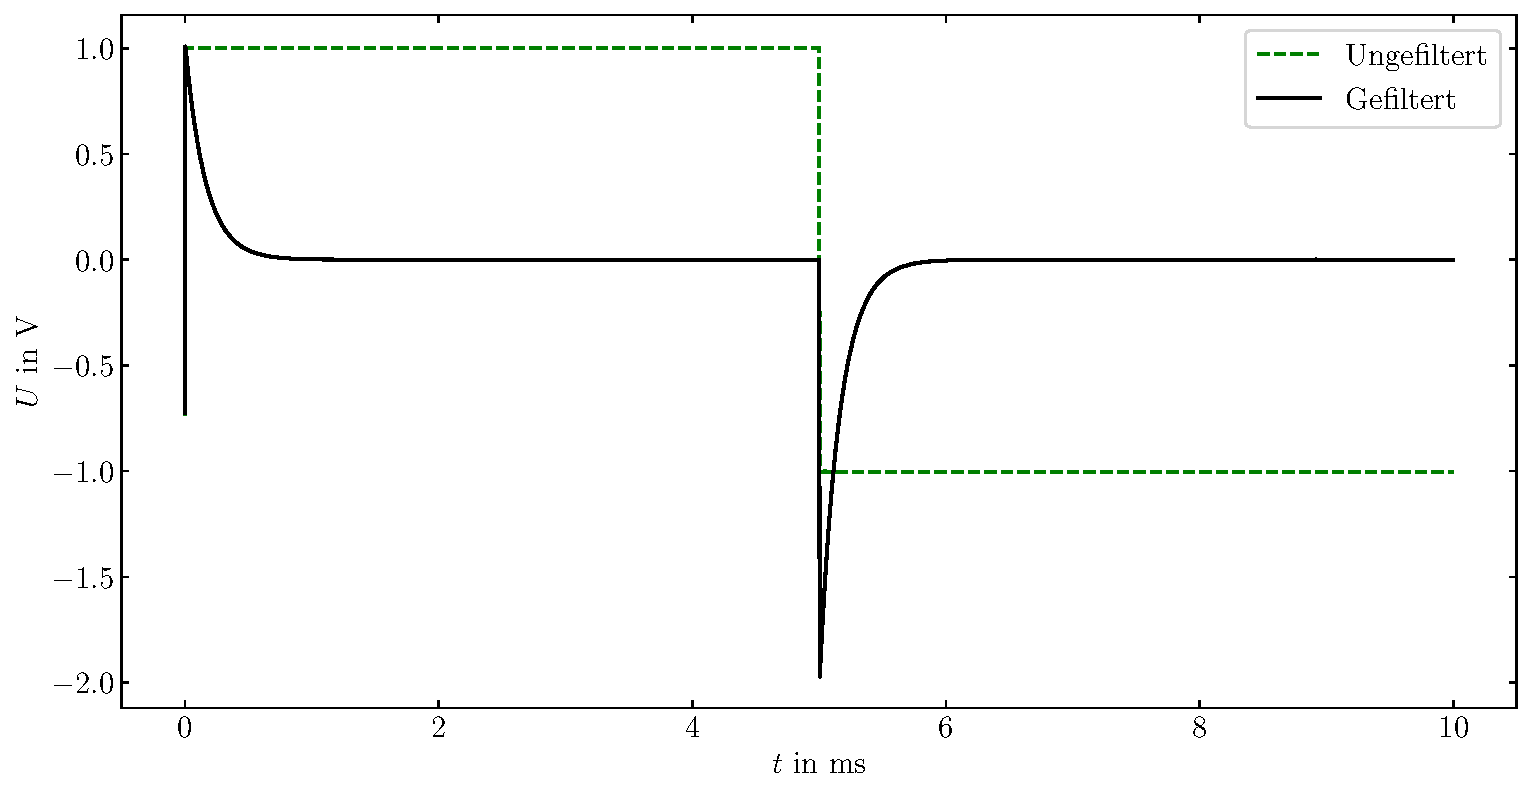
\includegraphics[width=\textwidth]{Paul/43bBuHi1S.pdf}
        \caption{Signal}
    \end{subfigure}
    \\
    \begin{subfigure}{0.9\textwidth}
        \centering
        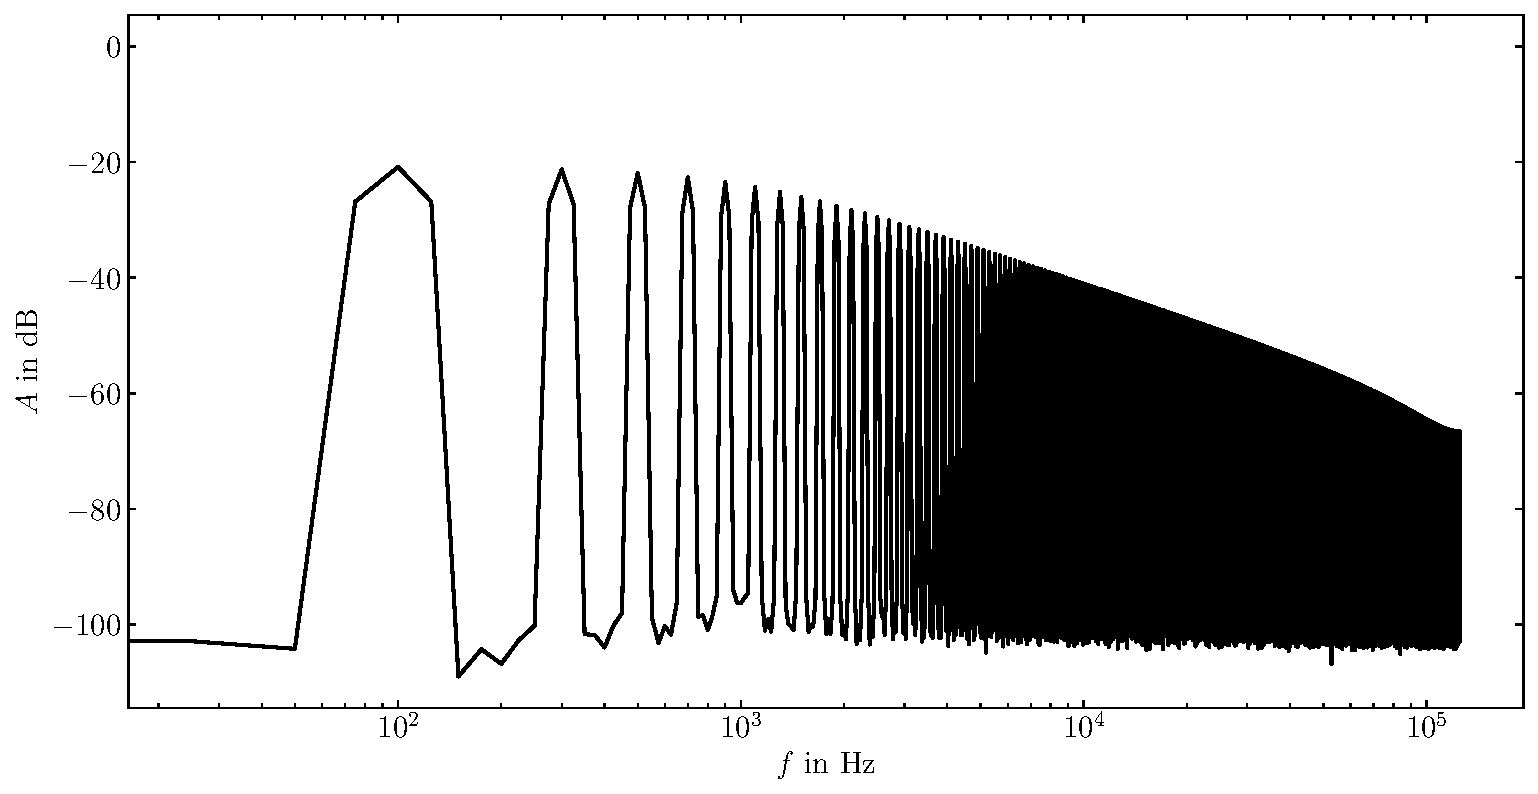
\includegraphics[width=\textwidth]{Paul/43bBuHi1F.pdf}
        \caption{Fourierspektrum}
    \end{subfigure}
    \caption{Butterworthfilter als Hochpass}
    \label{fig:43bBuHi1}
\end{figure}

Aus Abbildung \ref{fig:43bBuHi1} geht klar die differenzierende Eigenschaft des Hochpasses hervor. Außerdem knickt das Fourierspektrum für große Frequenzen ab.\\

\begin{figure}[h]
    \centering
    \begin{subfigure}{0.9\textwidth}
        \centering
        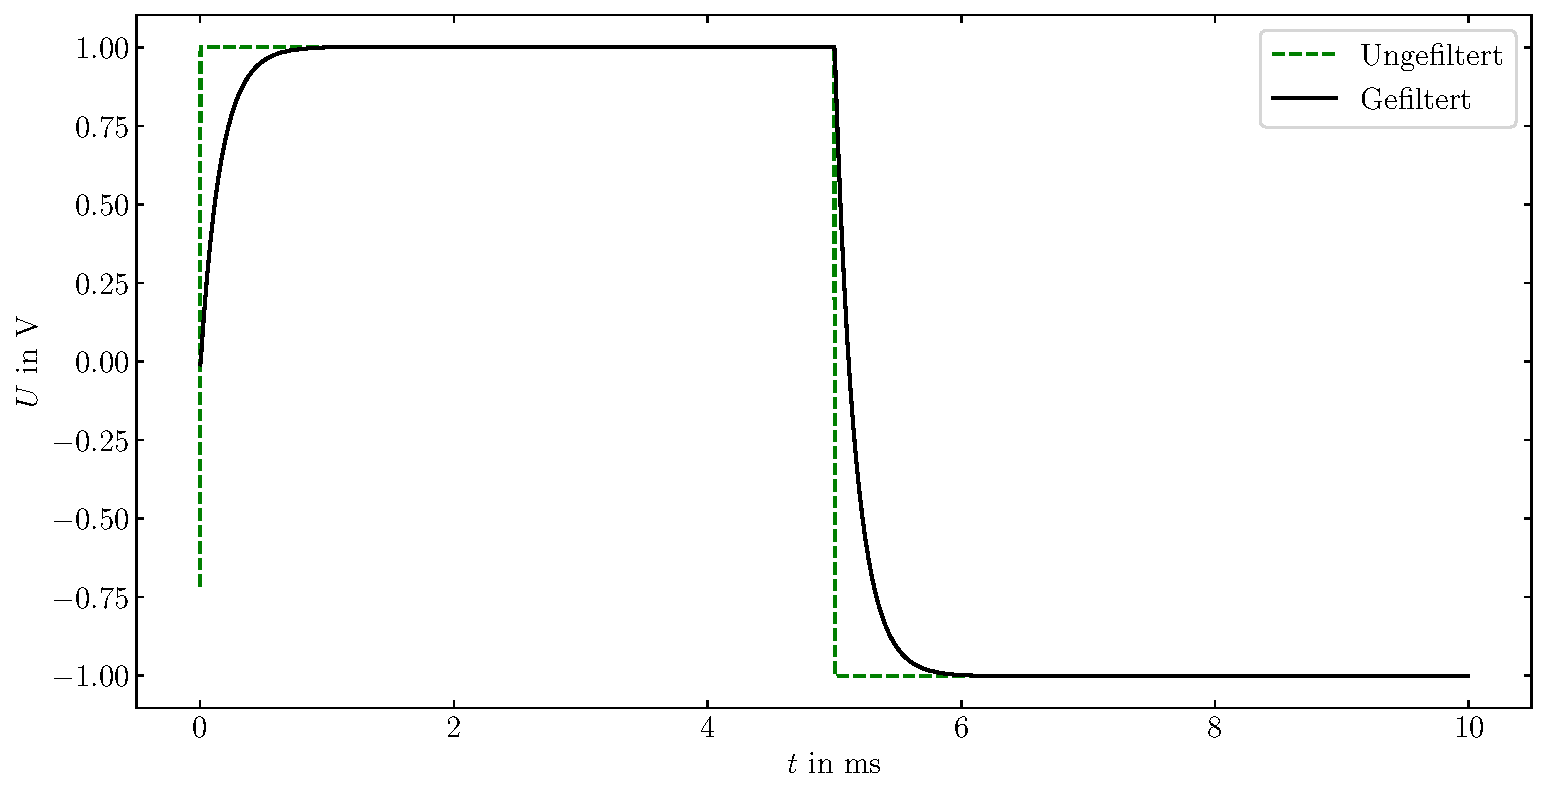
\includegraphics[width=\textwidth]{Paul/43bBuLo1S.pdf}
        \caption{Signal}
    \end{subfigure}
    \\
    \begin{subfigure}{0.9\textwidth}
        \centering
        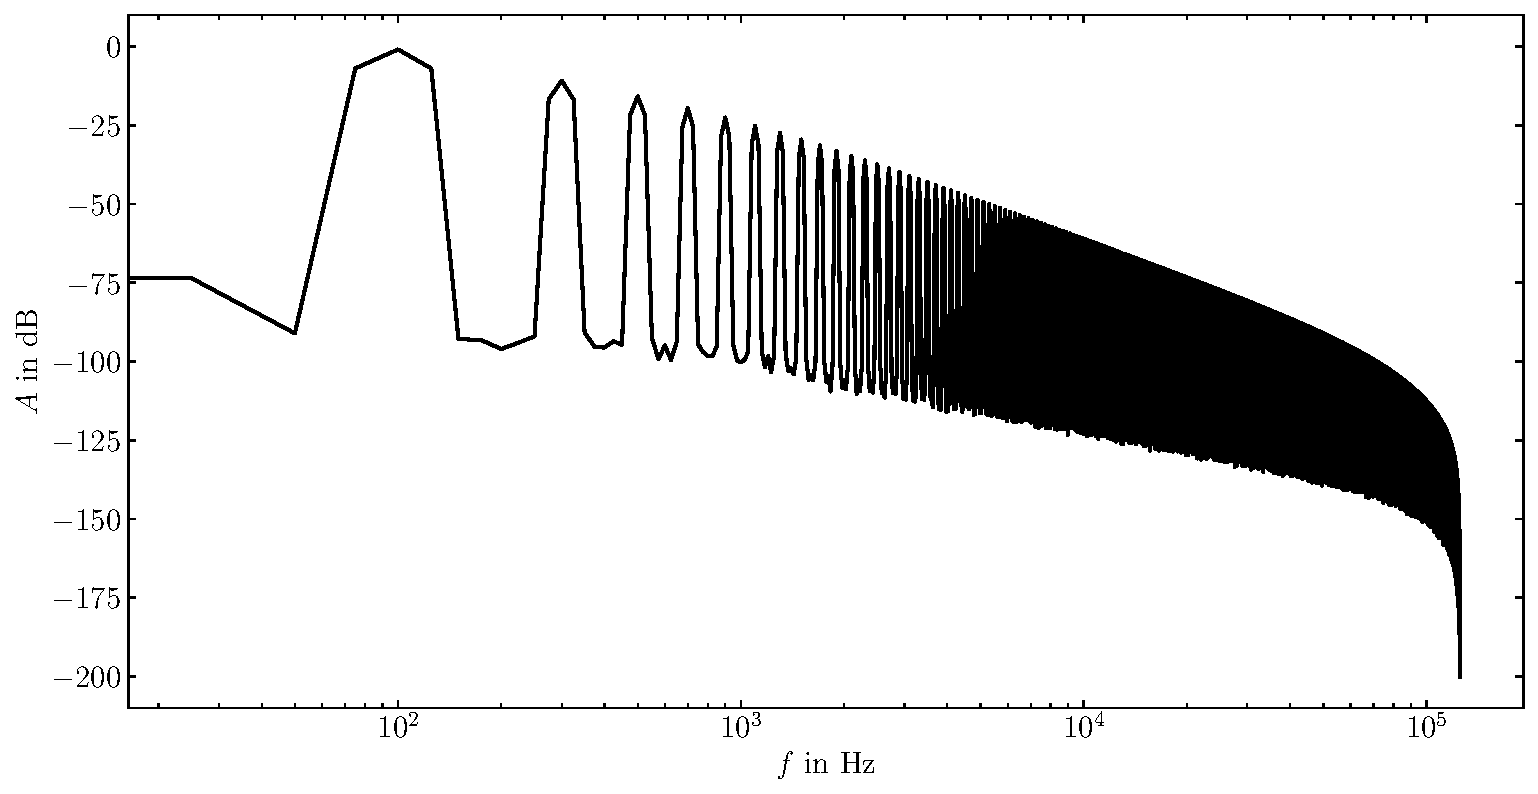
\includegraphics[width=\textwidth]{Paul/43bBuLo1F.pdf}
        \caption{Fourierspektrum}
    \end{subfigure}
    \caption{Butterworthfilter als Tiefpass}
    \label{fig:43BuLo1}
\end{figure}

Im Gegensatz zum Hochpass wirkt der Butterworthfilter Tiefpass als Integriere und das Fourierspektrum knickt für große Frequenzen ab, dies ist in Abbildung \ref{fig:43BuLo1} zu erkennen.


\newpage
Der inverse Chebyshevfilter zeigt vor allem im Signal ein ganz anderes Bild.\\
In Abbildung \ref{fig:43bInChHi1} ist beim Signal in der ersten Millisekunde eine gewisse Welligkeit zu erkennen. Im Bezug auf das Fourierspektrum fällt auf das dieser Filter, im Vergleich zum Butterworthhochpass, für größere Frequenzen schneller durchlässiger wird.
\begin{figure}[h]
    \centering
    \begin{subfigure}{0.9\textwidth}
        \centering
        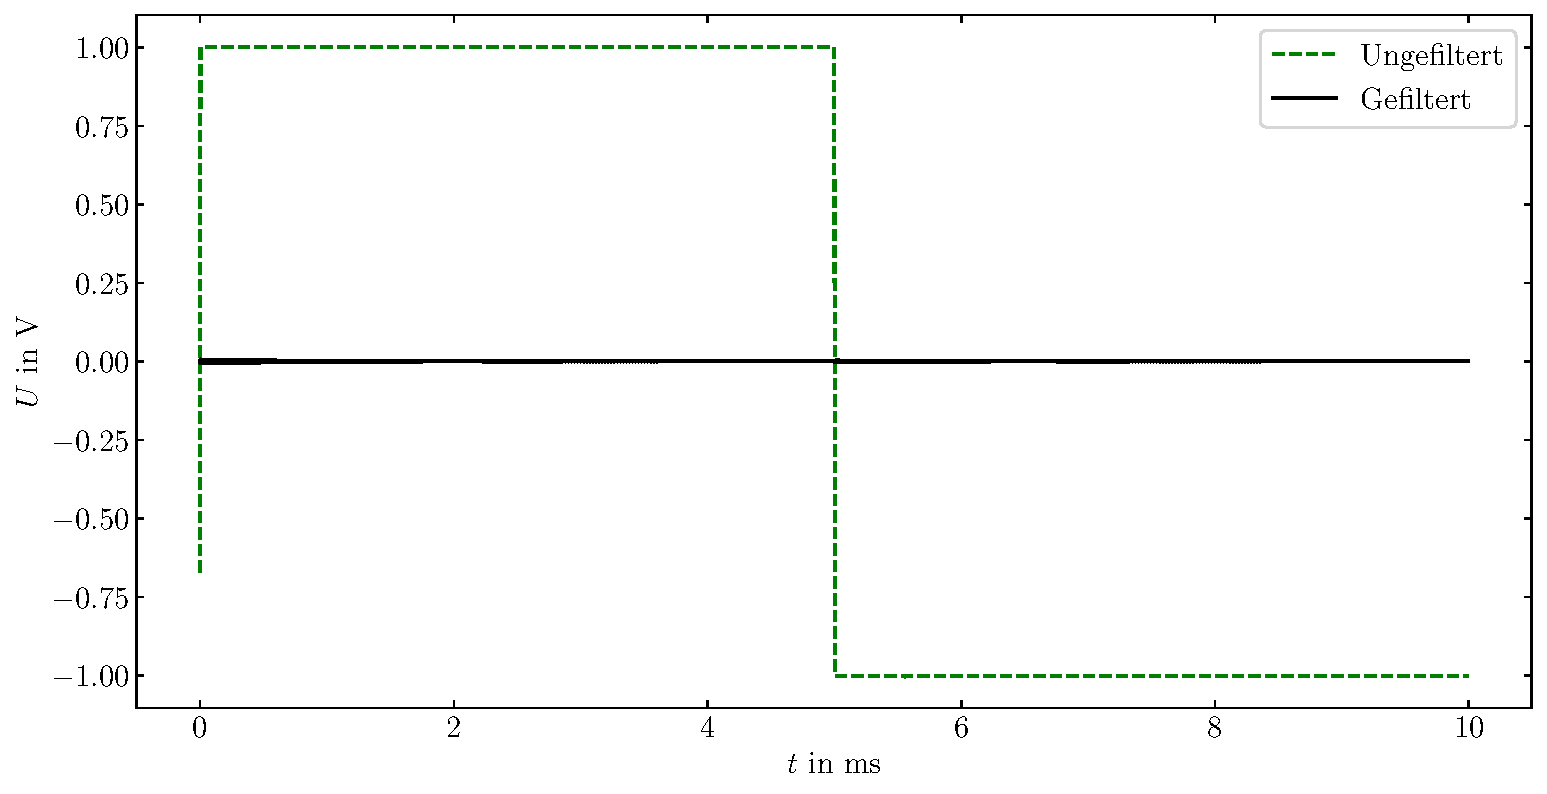
\includegraphics[width=\textwidth]{Paul/43bInChHi1S.pdf}
        \caption{Signal}
    \end{subfigure}
    \\
    \begin{subfigure}{0.9\textwidth}
        \centering
        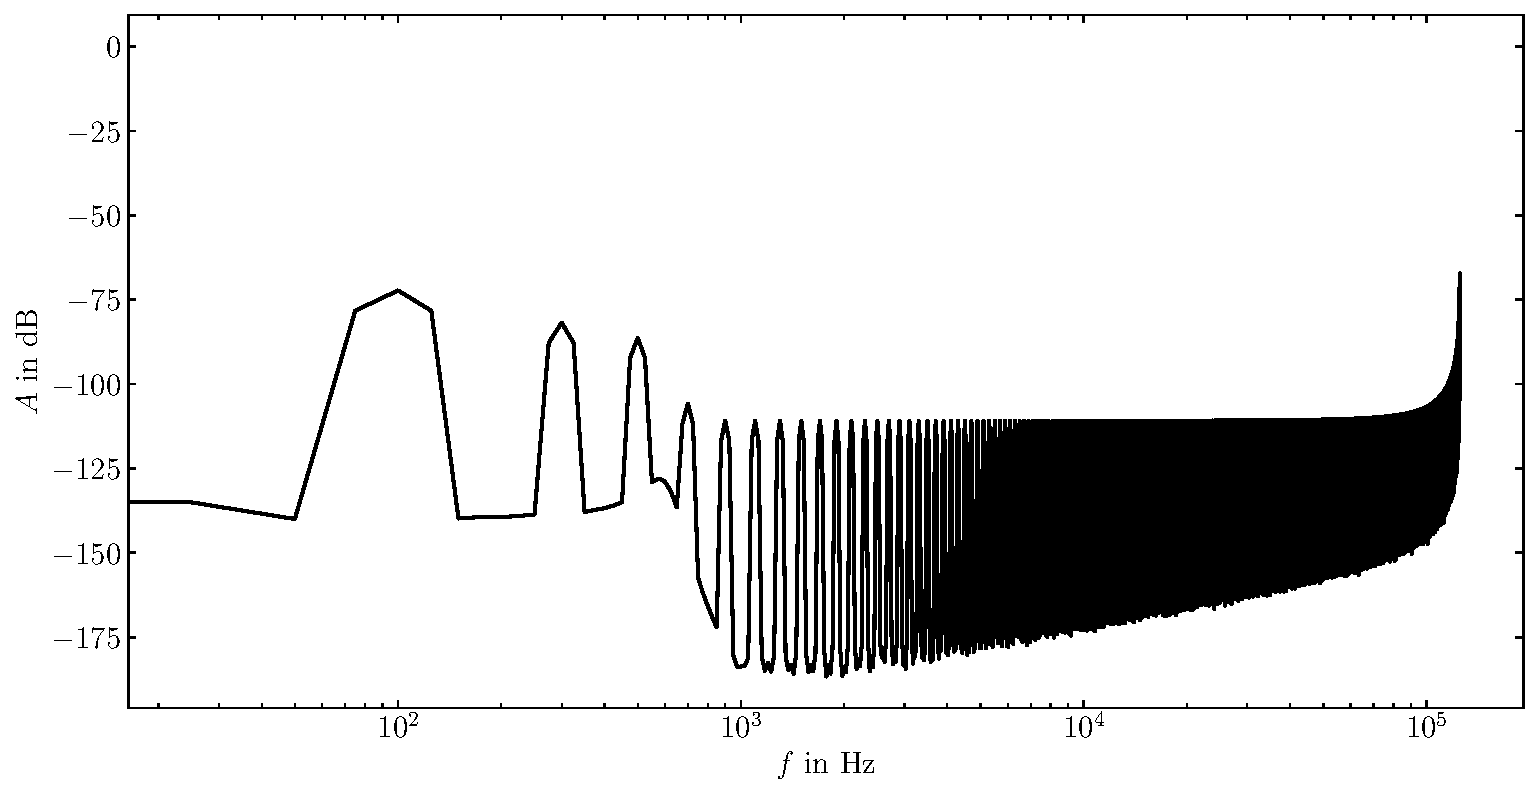
\includegraphics[width=\textwidth]{Paul/43bInChHi1F.pdf}
        \caption{Fourierspektrum}
    \end{subfigure}
    \caption{Inverser Chebyshevfilter als Hochpass}
    \label{fig:43bInChHi1}
\end{figure}

\newpage
In Abbildung \ref{fig:43bInChLo1} fällt die konstante Nulllinie beim gefilterten Signal auf, auch ist das abknicken (bei ca. 1 kHz), im Vergleich zum Butterworthtiefpass ausgeprägter.\\

\begin{figure}[h]
    \centering
    \begin{subfigure}{0.9\textwidth}
        \centering
        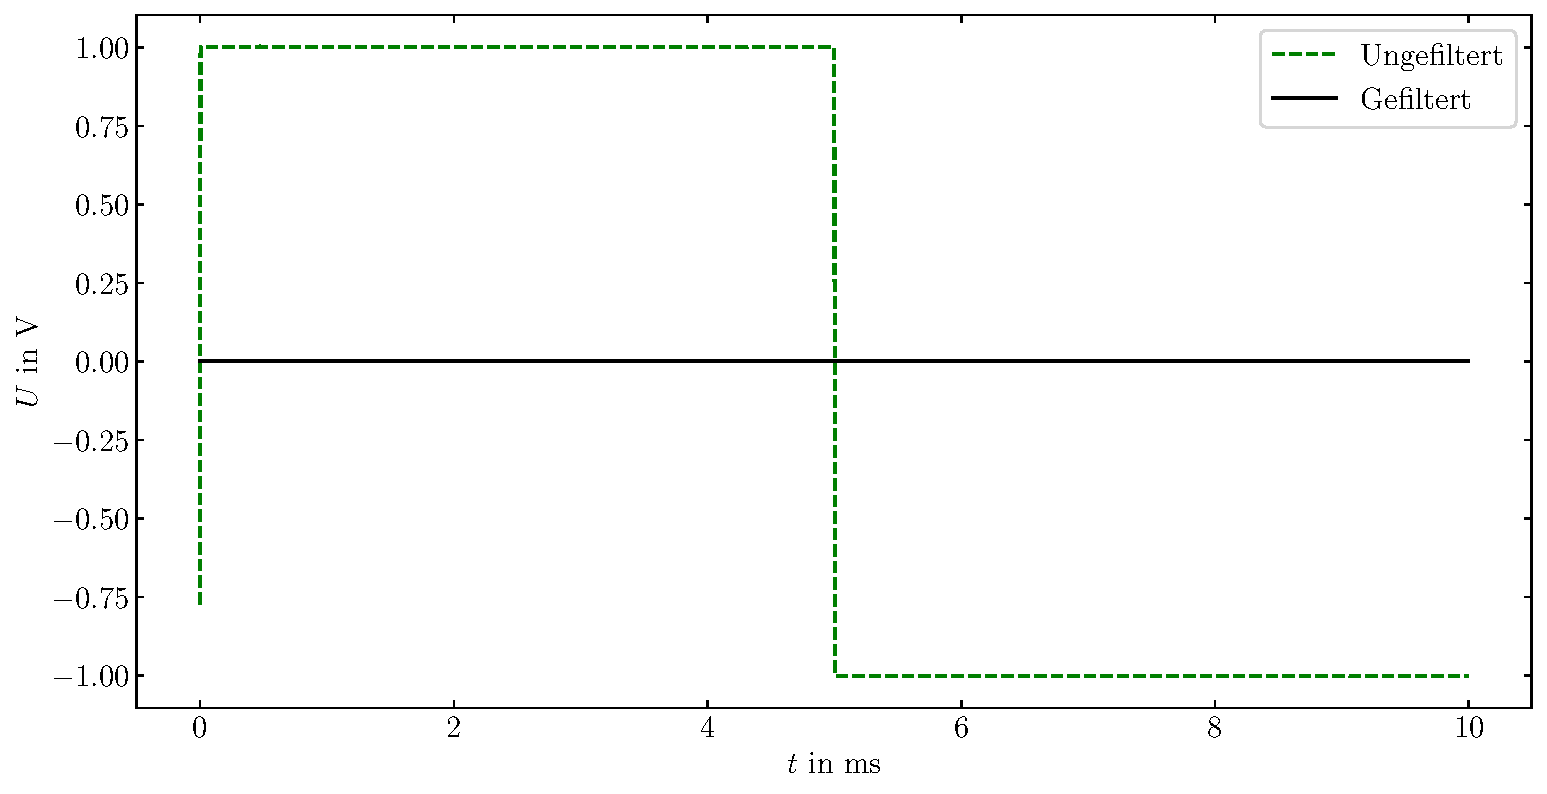
\includegraphics[width=\textwidth]{Paul/43bInChLo1S.pdf}
        \caption{Signal}
    \end{subfigure}
    \\
    \begin{subfigure}{0.9\textwidth}
        \centering
        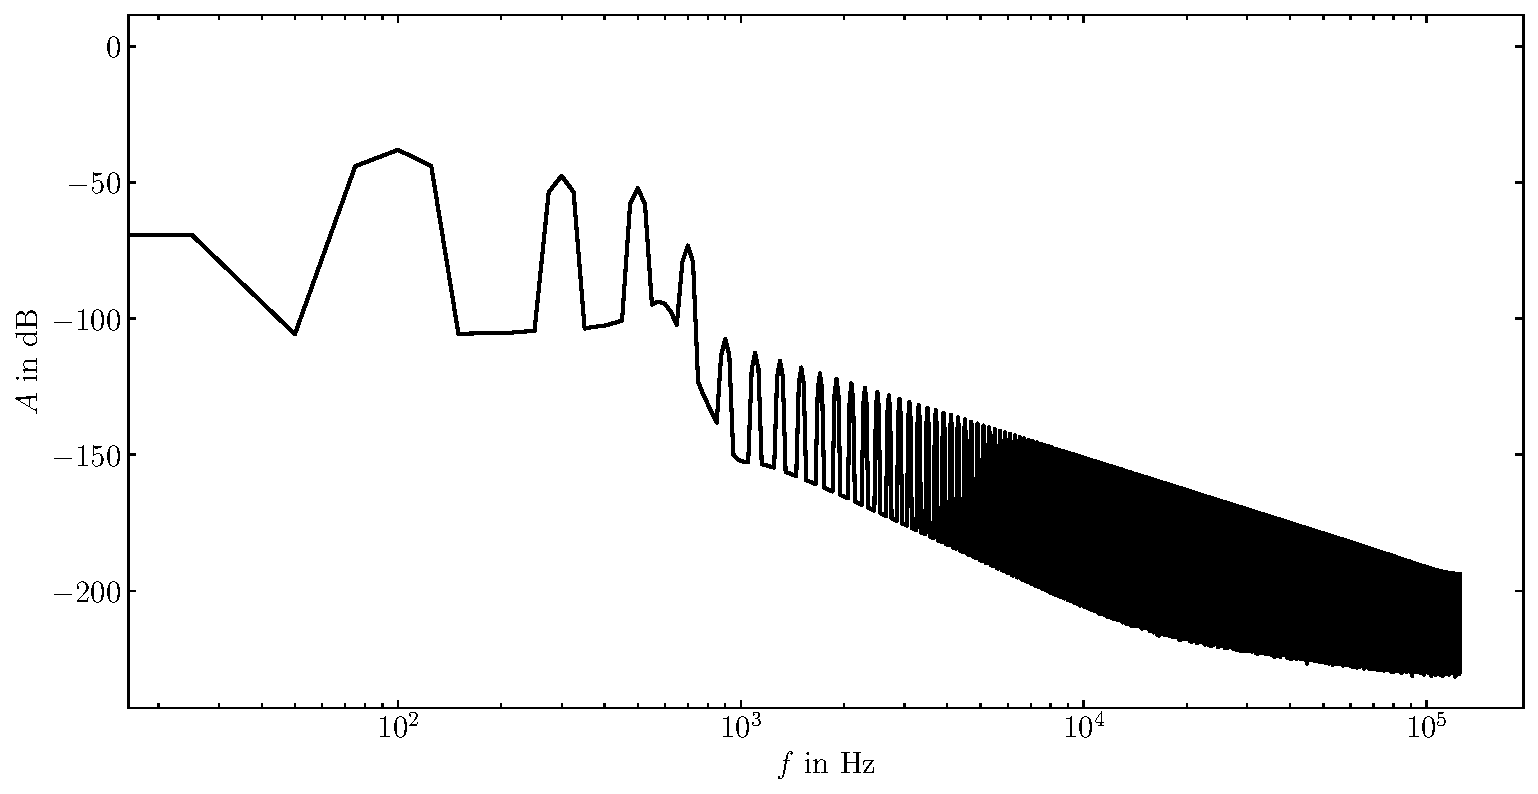
\includegraphics[width=\textwidth]{Paul/43bInChLo1F.pdf}
        \caption{Fourierspektrum}
    \end{subfigure}
    \caption{Inverser Chebyshevfilter als Tiefpass}
    \label{fig:43bInChLo1}
\end{figure}

Da die anderen Filter ähnliche Eigenschaften wie der Butterworthfilter aufweisen wurde auf die Abbildung deren Signale und Fourierspektren bewusst verzichtet.\\

\newpage
\subsection{Bandpass 4. Ordnung}

In diesem Abschnitt soll die geeignete Einstellung eines Butterworthbandpasses (4. Ordnung) gefunden werden, die Rauschen, beim gleichzeitigen Erhalt der zeitlichen Form der Signalfunktion, abmildert.
\begin{figure}[h]
    \centering
    \begin{subfigure}{0.9\textwidth}
        \centering
        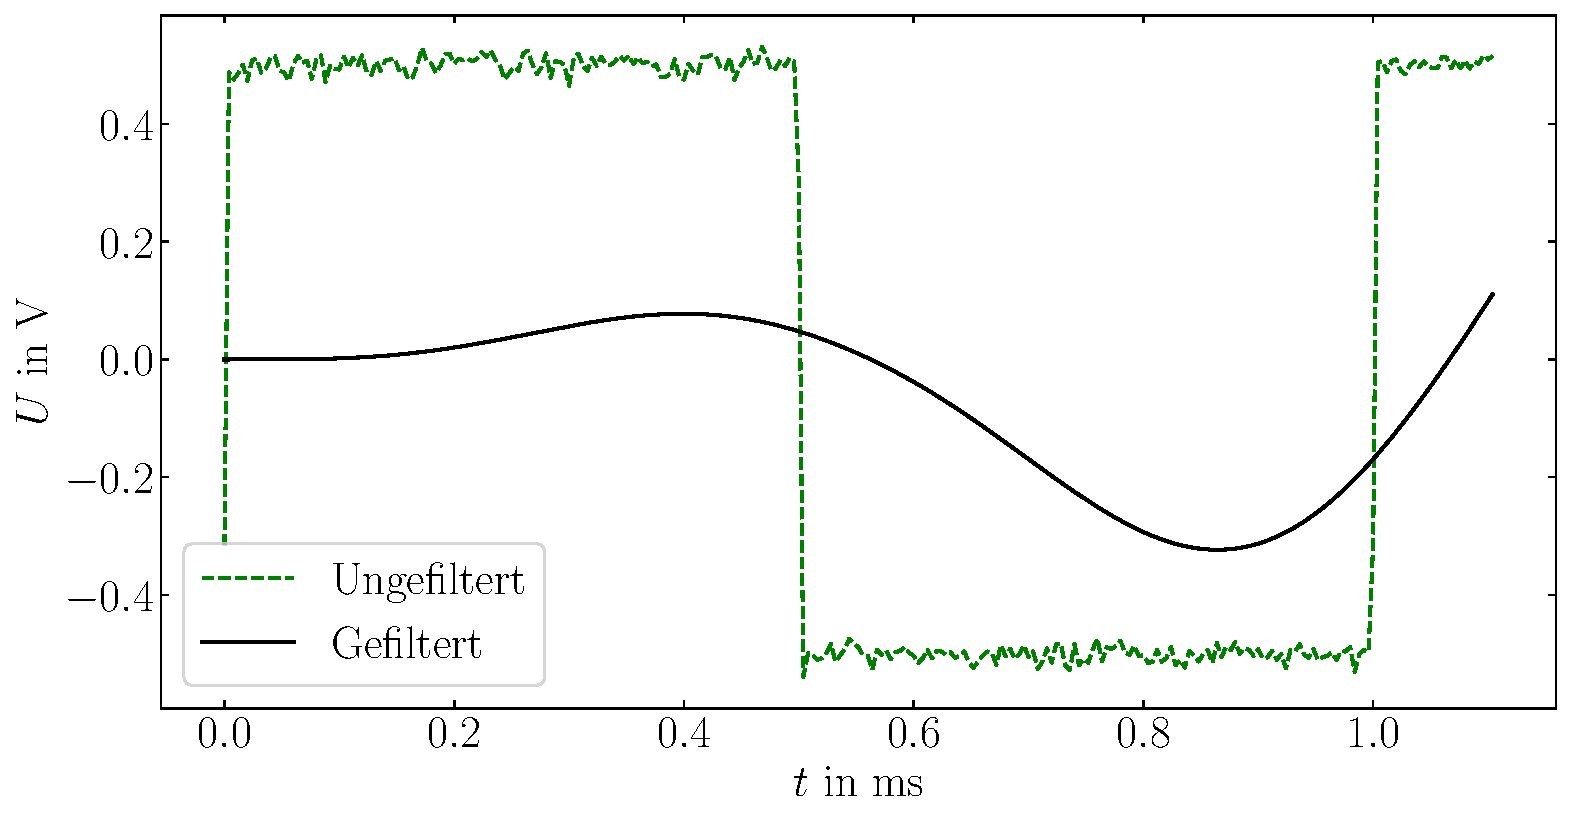
\includegraphics[width=\textwidth]{Paul/43cLf500Hf1500S.pdf}
        \caption{Bandpass mit Durchlassbereich von 500 bis 1500Hz}
    \end{subfigure}
    \\
    \begin{subfigure}{0.9\textwidth}
        \centering
        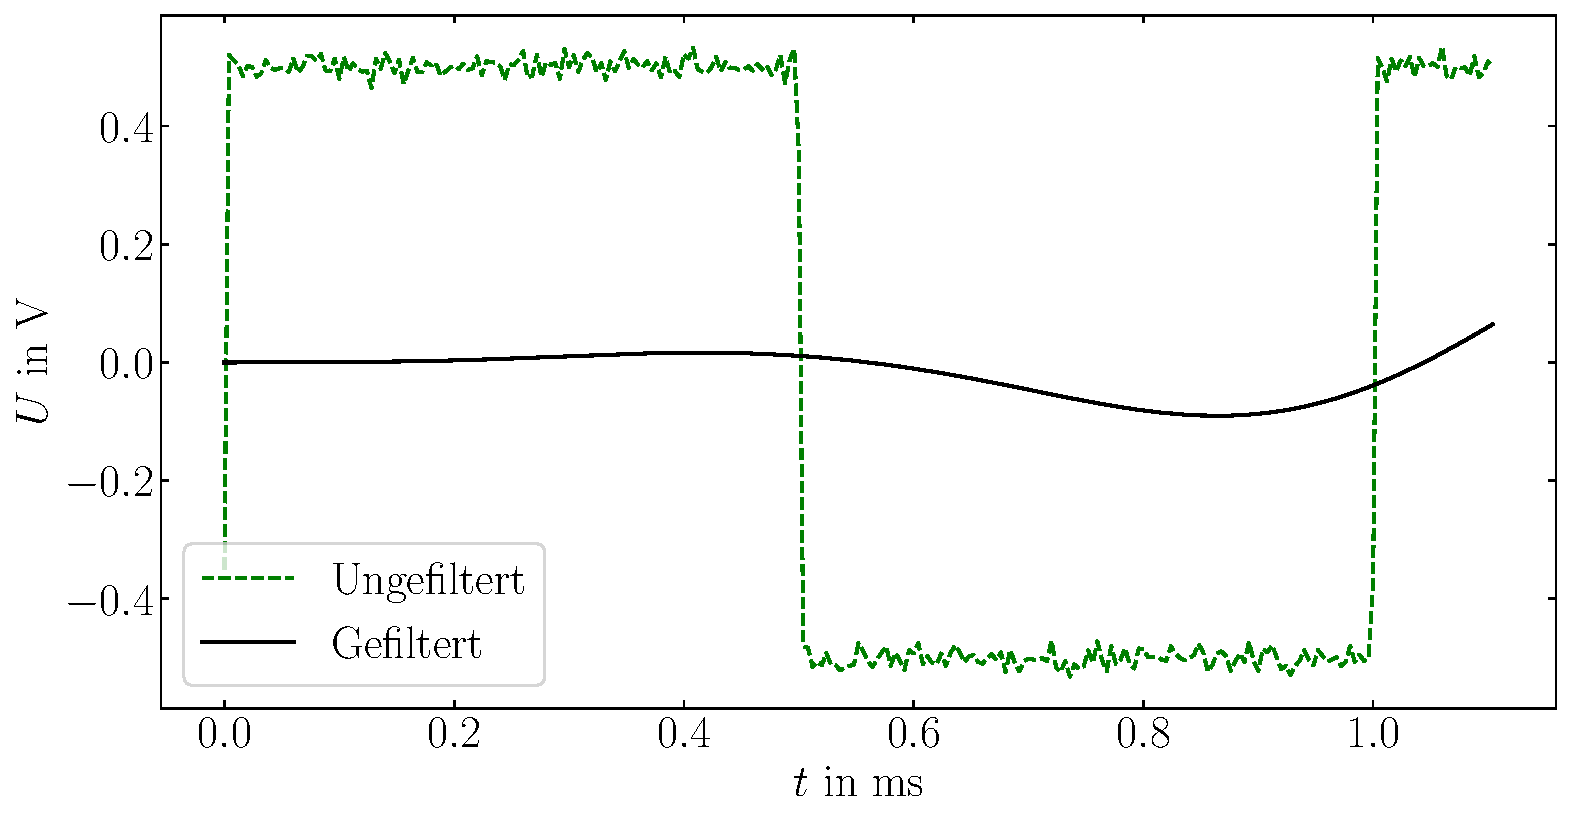
\includegraphics[width=\textwidth]{Paul/43cLf700Hf1300S.pdf}
        \caption{Bandpass mit Durchlassbereich von 700 bis 1300Hz}
    \end{subfigure}
    \caption{Signalfunktion verschiedener Bandpässe}
    \label{fig:43cverBa}
\end{figure}

Die in Abbildung \ref{fig:43cverBa} gezeigten Signalfunktionen weichen stark von einer Rechteckfunktion ab und sind daher ungeeignet.\\
Durch weiteres Ausprobieren wurden bessere Einstellungen gefunden, welche die in Abbildung \ref{fig:43cBeBa} dargestellte Signalfunktion ergeben. Hier ist noch deutlich ein Rechtecksignal zu erkennen.\\

\begin{figure}[h]
    \centering
    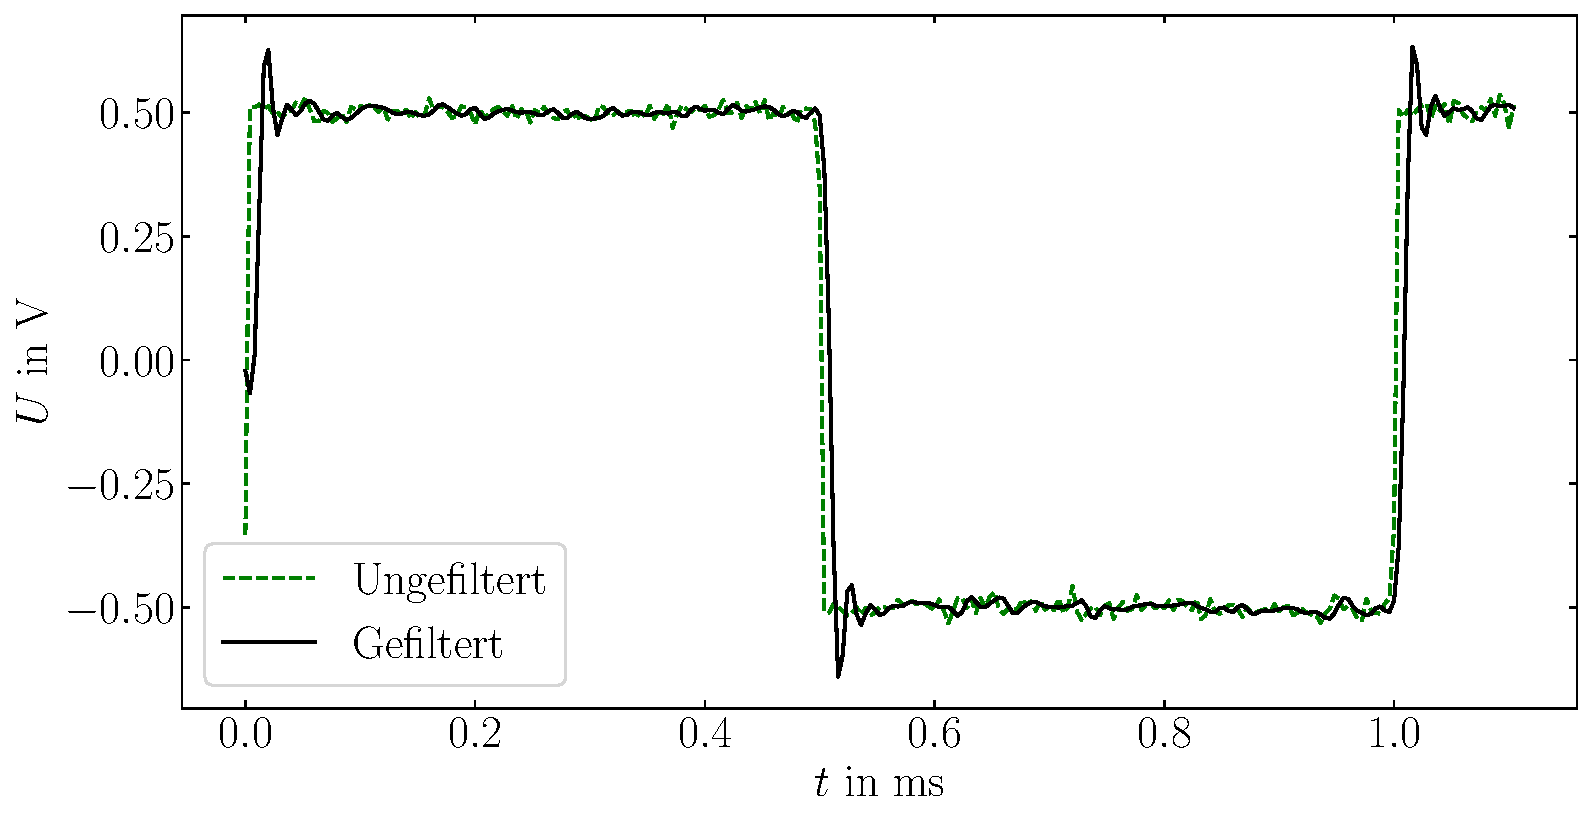
\includegraphics[width=\textwidth]{Paul/43cLf10mHz55kHzS.pdf}
    \caption{Bandpass mit Durchlassbereich von 10mHz bis 55kHz}
    \label{fig:43cBeBa}
\end{figure}

Eine gute Rauschunterdrückung verursacht also eine große Signalverzerrung. Der Grund hierfür ist folgender: Die Fouriertransformierte des Rechtecksignals ist eine Superposition von Sinusschwingungen über den ganzen Frequenzraum, wenn nun ein Teil dieser Frequenzen herausgefiltert werden und eine Rücktransformation erfolgt kommt es, aufgrund der fehlenden Frequenzen zu einer Signalverzerrung. Das heist um so enger der Bandpass eingestellt wird um so verzehrter wird das Rechtecksignal, was gut zu unseren Beobachtungen passt. Es ist also darauf zu achten, dass dieses Verhältnis, abhängig vom Fokus der Messung, klug gewählt wird.

\newpage
\subsection{Einfluss der Ordnung}
\label{chap:Einfl-d-Ord}
Im folgenden soll betrachtet werden welchen Einfluss die Ordnung eines Filters hat.
Um diesen Umstand genauer betrachten zu können werden Fourierspektren von Filtern verschiedener Ordnung miteinander verglichen.
\begin{figure}[h]
    \centering
    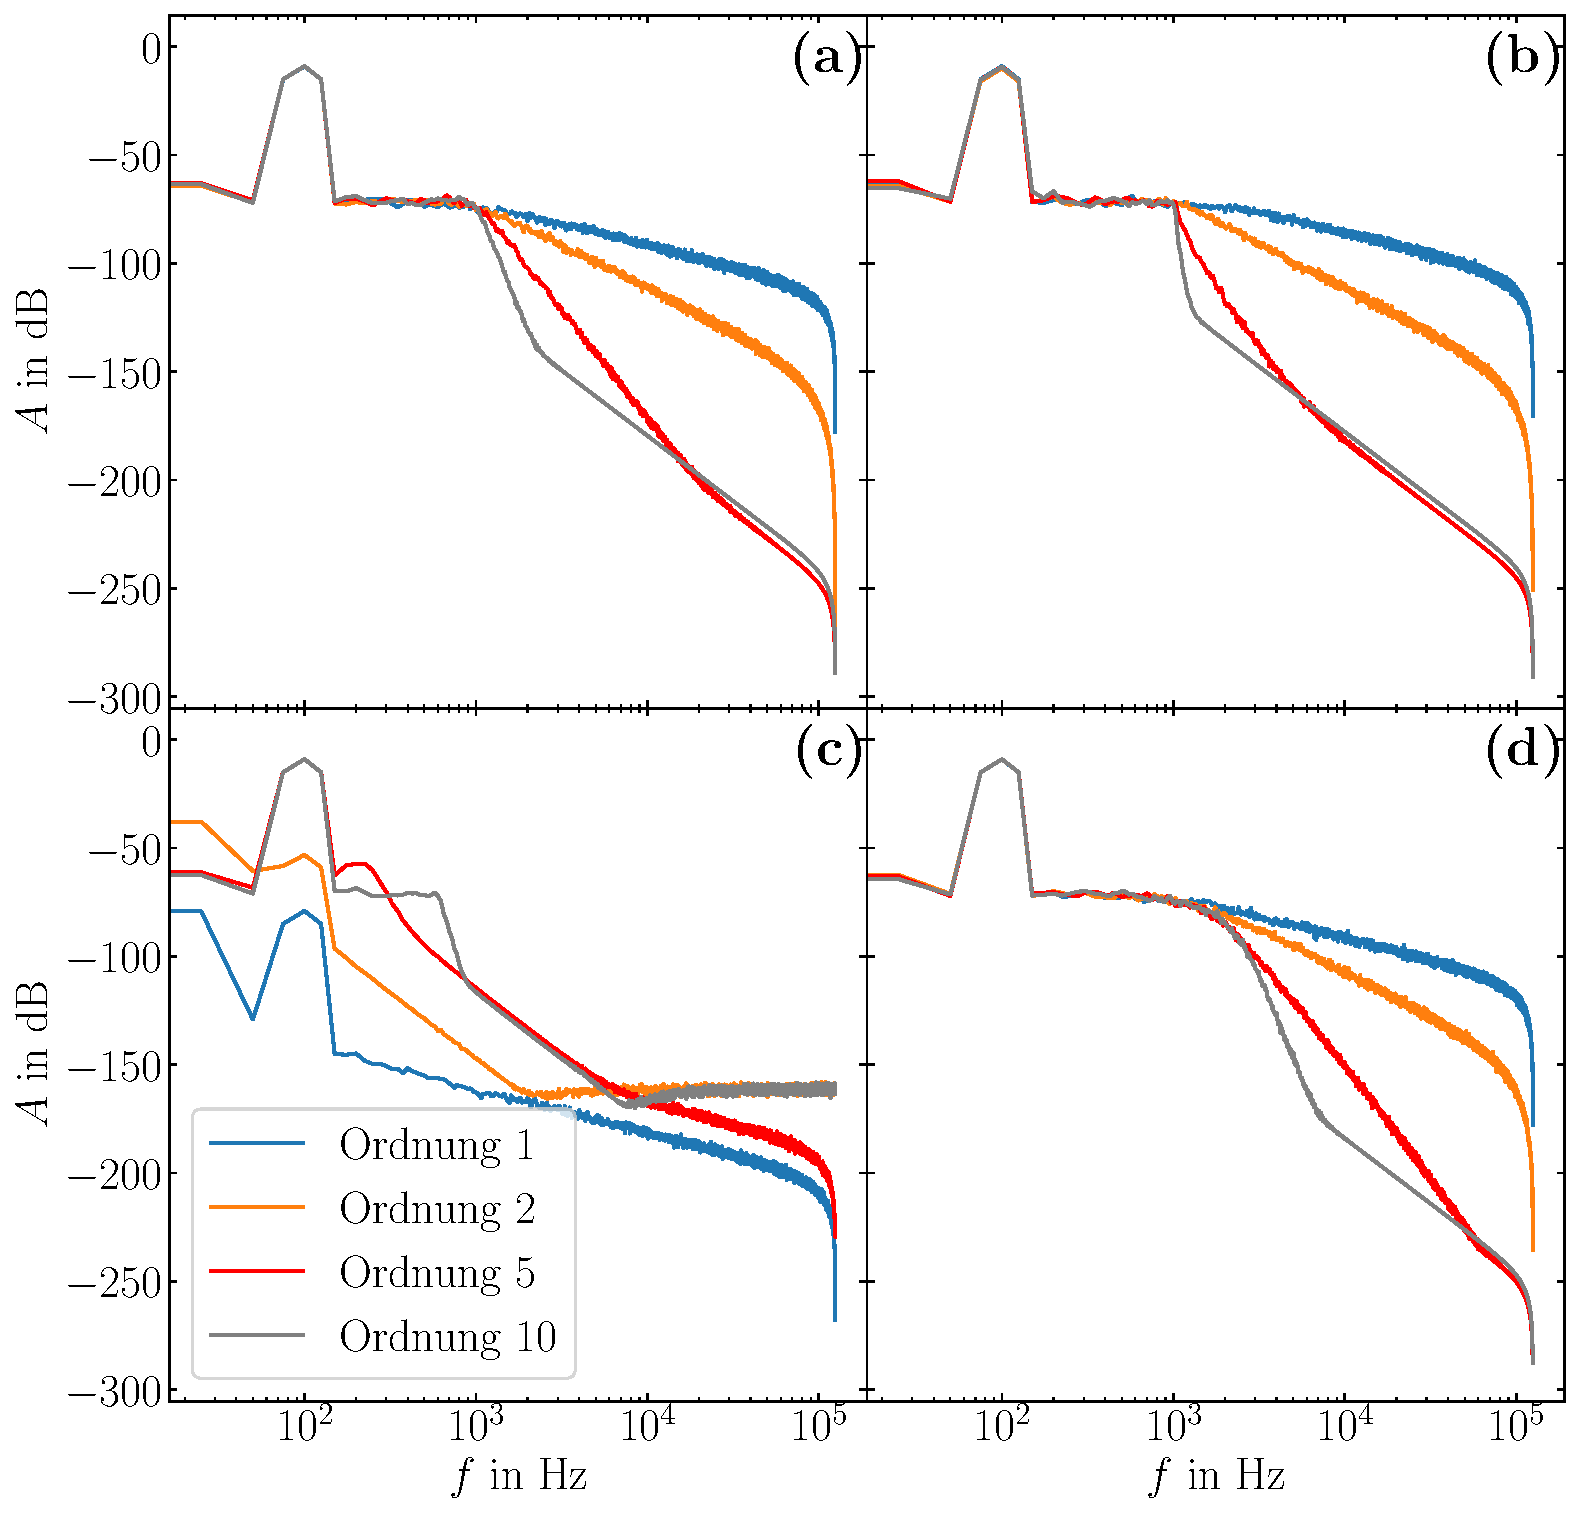
\includegraphics[scale = 0.5]{Paul/43dAllFilAll.pdf}
    \caption{(a) Butterworth, (b) Chebyshev, (c) Inverse Chebyshev und (d) Besselfilter bei verschiedenen Ordnungen}
    \label{fig:43dOrd}
\end{figure}

Aus Abbildung \ref{fig:43dOrd} ist zu erkennen, dass mit höherer Ordnung die Kurve, nach dem Knick, steiler Abfällt.
Für große Ordnungen fällt jedoch ein weiterer Knick bei höheren Frequenzen auf, welcher die Kurve danach abflacht. Außerdem sind alle Filter im Durchlassbereich, unabhängig von der Ordnung, deckungsgleich, bis auf den Inversen Chebyshev. Beim Inversen Chebyshev ist auch noch zu beobachten, dass für gerade Ordnungen, die Kurve im letzten Teil des Frequenzspektrums waagrecht verläuft.

\newpage
\subsection{Vergleich: Analoge und digitale Filterung}
Um die analoge mit der digitalen Filterung zu Vergleichen wird zuerst eine Messung mit dem gewohntem Messaufbau für den digitalen Filter aufgenommen. Danach wird der digitale Filter über die Messsoftware deaktiviert und zwischen den Generator und Detektor wird ein analoger Filter (Modell: Ithaco 4302) geschaltet, der analog zum digitalen Filter eingestellt wurde.

\begin{figure}[h]
    \centering
    \begin{subfigure}{0.9\textwidth}
        \centering
        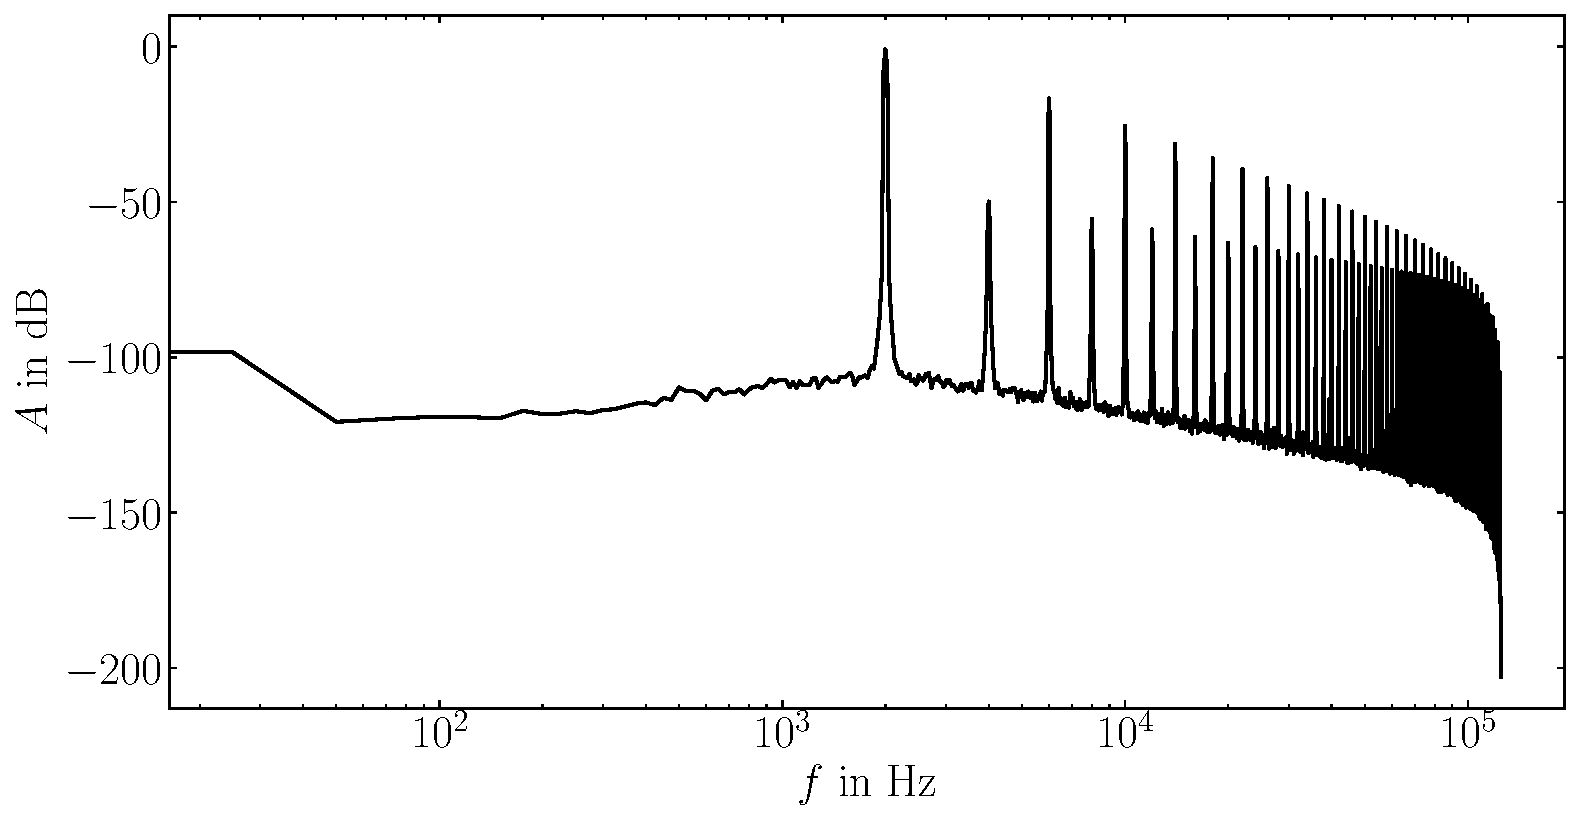
\includegraphics[width=\textwidth]{Paul/43eDF.pdf}
        \caption{digitale Filterung}
    \end{subfigure}
    \\
    \begin{subfigure}{0.9\textwidth}
        \centering
        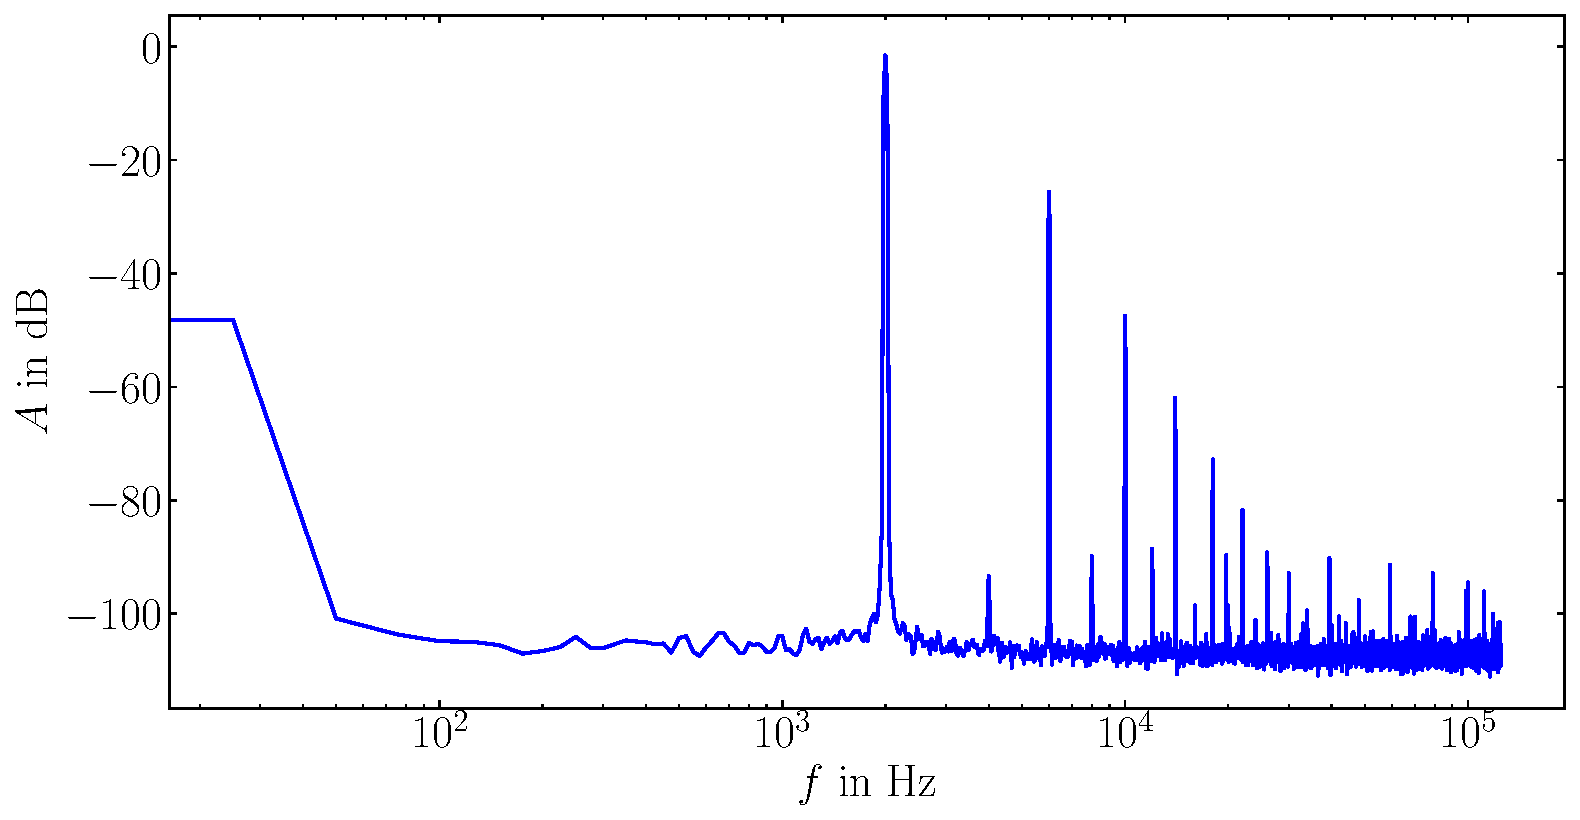
\includegraphics[width=\textwidth]{Paul/43eAF.pdf}
        \caption{analoge Filterung}
    \end{subfigure}
    \caption{Vergleich von analoger und digitaler Filterung}
    \label{fig:43e}
\end{figure}
\newpage
In Abbildung \ref{fig:43e} sind die Fourierspektren nach analoger und digitaler Filterung aufgetragen. Vergleicht man beides, so fällt auf, dass bei der digitalen Filterung auch der Hintergrund die Charakteristik des Bandpasses zeigt, wohingegen bei der analogen Filterung scheinbar nur die Nebenmaxima betroffen sind.\\
Eine mögliche Erklärung wäre, dass der Hintergrund nach dem analogen Filter einkoppelt oder das diese Eigenschaft eine Eigenschaft des analogen Filters ist, bzw. die Auflösung der Filter ab -100dB abnimmt. (Aus Gründen der Übersichtlichkeit wurde darauf verzichtet, die Kurven in einen einzigen Plot aufzuzeichnen.)


\subsection{Vergleich Filterung und Mittelung}
Wenn man Filterung und Mittelung gegenüberstellt, so ist der größte Unterschied wohl das beim Filtern aktiv bestimmte Frequenzen unterdrückt werden, je nach Einstellung bzw. Dimensionierung des Filters. Dies kann dabei helfen, dass das Messsignal von Störungen wie dem 50\,Hz Brummen bereinigt werden kann.\\
Mitteln hingegen ist besonders geeignet um die Messung von bspw. weißes Rauschen zu bereinigen da dies, gemittelt über die Zeit, Null ergibt.
\newpage
% Teilauswertung 4

\section{Lock-In Verstärker}
\label{sec:lockin}

\paragraph{a)}\textbf{Lock-In Verstärker als Filter}

Im folgenden Teil der Lock-In Verstärker als Filter verwenden und die Ausgangsmesswerte der Sinus, Rechteck und Dreieckschwingung interpretieren.

Die Messungen haben folgende Tabelle ergeben:
\begin{center}
    \begin{tabular}{l | c c c c c c c}
        f/kHz               & 1 & 3 & 5 & 7 & 9 & 11 & 13 \\
        \hline
        $U_{eff,Sinus}$/V     & 0,7072 & 0,0000 & 0,0000 & 0,0000 & 0,0000 & 0,0000 & 0,0000 \\
        $U_{eff,Rechteck}$/V  & 0,9003 & 0,3000 & 0,1800 & 0,1285 & 0,1000 & 0,0817 & 0,0692 \\
        $U_{eff,Dreieck}$/V   & 0,5733 & 0,0636 & 0,0229 & 0,0117 & 0,0070 & 0,0047 & 0,0034 \\
    \end{tabular}
    \captionof{table}{Messung Lock-In Verstärker als Filter bei unterschiedlichen Signalen}
    \label{tab:lockinFilter}
\end{center}
Wie in Tabelle \ref{tab:lockinFilter} schon angedeutet, handelt es sich bei den gemessenen Spannungswerte um die Effektivspannungswerte der jeweiligen Schwingung. Wie schon in Kapitel \ref{sec:mittelungAndTrafo}a) kann man die Effektivspannungswerte in die Werte der Fourierentwicklungskoeffizienten umrechnen, indem man die Messwerte mit dem Faktor $\sqrt{2}$ multipliziert. Zum Vergleich mit der Theorie werden die errechneten Werte aus Tabelle \ref{tab:fourierkoeff} verwendet und es werden wieder nur Rechteck- und Dreieckschwingung betrachtet. Weiterhin wird erneut die betragsmässige Differenz wie in Kapitel \ref{sec:fourierseries}a) berechnet. Damit erhält man:
\begin{center}
    \begin{tabular}{c | c c r | c c r}
        {} & \multicolumn{3}{c|}{\textbf{Rechteck}} & \multicolumn{3}{c}{\textbf{Dreieck}}\\
        $f$/kHz & $U_{Mess}$/V & $U_{Theo}$/V & $\Delta U$/$\mu$V & $U_{Mess}$/V & $U_{Theo}$/V & $\Delta U$/$\mu$V\\
        \hline
         1  & 1.273216 &  1.273240 &   23.07 &   0.810769 &   0.810569 &  199.17 \\
         3  & 0.424264 &  0.424413 &  149.11 &   0.089944 &   0.090063 &  119.29 \\
         5  & 0.254558 &  0.254648 &   89.47 &   0.032385 &   0.032423 &   37.29 \\
         7  & 0.181726 &  0.181891 &  164.92 &   0.016546 &   0.016542 &    4.06 \\
         9  & 0.141421 &  0.141471 &   49.70 &   0.009899 &   0.010007 &  107.54 \\
        11  & 0.115541 &  0.115749 &  207.80 &   0.006647 &   0.006699 &   52.12 \\
        13  & 0.097864 &  0.097942 &   77.92 &   0.004808 &   0.004796 &   12.06 \\
    \end{tabular}
    \captionof{table}{Vergleich Theorie und Praxis bei der Messung mit Lock-In Verstärker}
    \label{tab:lockinFourierkoeff}
\end{center} 
In Tabelle \ref{tab:lockinFourierkoeff} sieht man ganz deutlich wie präzise die Messung mit einem Lock-In Verstärkers ist. In der Berechnung hat man dabei bewusst auf die Fehlerrechnung verzichtet, da die Fehler nur in der Größenordnung von $\pm 0,0001$\,V liegen. Im Vergleich zu Tabelle \ref{tab:fourierkoeff} hat der Lock-In Verstärker aber eine deutlich höhere Präzession der Messung, da vor allem bei Frequenzen von 1\,kHz eine geringere Abweichung zu verzeichnen ist. Dies der Sachverhalt wurde im Verglaich mit den Ergebnis aus Kapitel \ref{sec:fourierseries}a) in Abbildung \ref{image:resiVergleich} dargestellt.
\begin{center}
    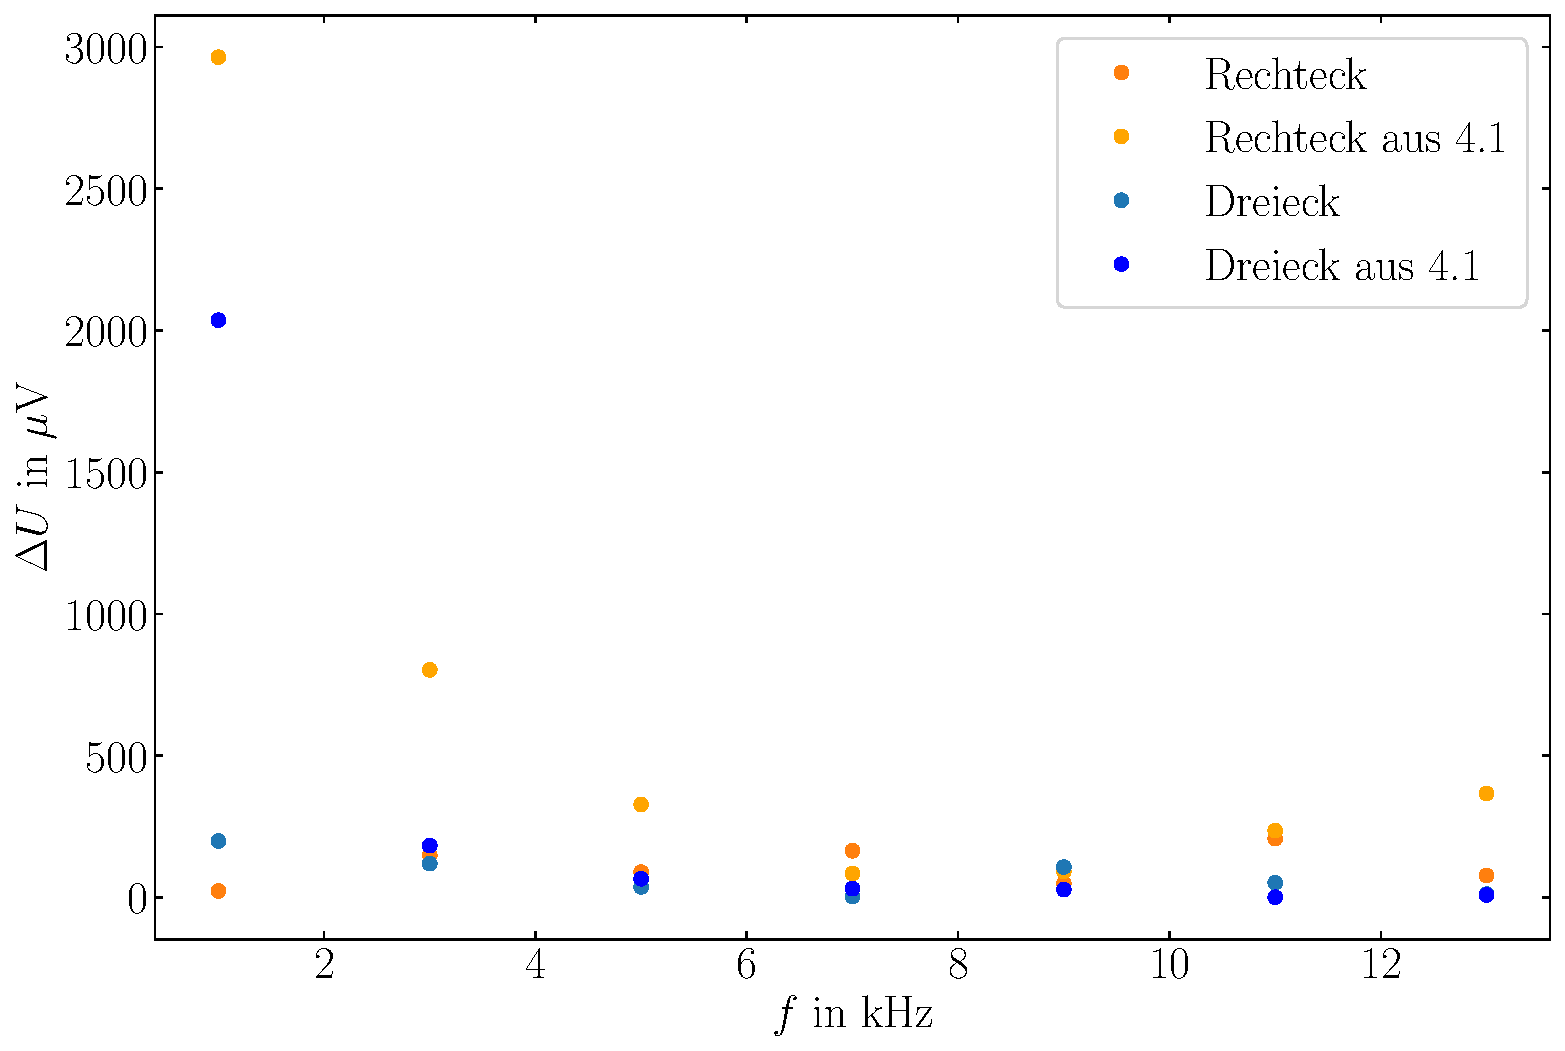
\includegraphics[scale=0.5]{Manuel/44/ResiduumVergleich.pdf}
    \captionof{figure}{Vergleich der betragsmässigen Differenz zwischen Ergebnis aus Kapitel 4.4a) und Kapitel 4.1a)}
    \label{image:resiVergleich}
\end{center} 

\newpage
\paragraph{b)}\textbf{Bandbreite des Lock-In Verstärkers}

Als Nächstes wird die Zeitkonstante $\tau$ und die Ordnung $n$ des Filters des Lock-In Verstärkers bestimmt. Dafür wurde an dem Lock-In Verstärker eine Sinusschwingung mit einer Frequenz von 1\,kHz und eine Amplitude von 100\,mV angelegt. Am Lock-In Verstärker wurde die Flankensteilheit $\Delta$ des eingebauten Tiefpassfilters von 6\,dB auf 18\,dB verändert und eine Zeitkonstante $\tau$ von 30\,ms eingestellt. Um die Zeitkonstante und Ordnung zu bestimmen wird eine Kurve durch die aufgenommene Messreihe gefittet. Die Form der Kurve wurde im Praktikum zur Verfügung besprochen und ist speziell für den Lock-In Verstärker SR830 DSP. Die Kurve hat dann die Gleichung:
\begin{gather}
    A_{\tau,n}(f) = \left[1 + (2\pi\tau(f-f_0))^2\right]^{-\frac{n}{2}}
\end{gather}
Diese Gleichung beschreibt hierbei die Filterantwort des Lock-In Verstärkers, wobei \newline $n$ die Ordnung, $\tau$ die Zeitkonstante des Filters und $A$ die normierte Amplitude ist. Die Frequenz $f_0$ ist die eingestellte Frequenz der Sinusschwingung und liegt bei 1kHz. Die Normierung erfolgt über den maximalen Wert der Effektivspannung, welcher bei den Frequenz $f_0$ liegt. Durch die Normierung muss die Umwandlung von Effektivspannung in tatsächliche Spannung nicht berücksichtigt werden. Es wurde wieder auf eine Fehlerrechnung verzichtet, da die Fehler der Messwerte zu klein sind. Der Fit liefert dann folgende Parameter:
\begin{center}
    \begin{tabular}{c | c c}
        $\Delta$/dB & $\tau$/ms & $n$\\
        \hline
        6  & 27,35 & 1,06 \\
        18 & 30,16 & 3,00 \\
    \end{tabular}
    \captionof{table}{Ergebnis gefittete Parameter für $\tau$ und $n$}
    \label{tab:fitPara}
\end{center}
In Abbildung \ref{image:6dB} und \ref{image:18dB} ist jeweils der Fit für die jeweilige Messreihe dargestellt. Der Vergleich der gefitteten Werte der Zeitkonstante $\tau$ mit dem tatsächlichen eingestellten Wert von 30ms zeigt, dass die Messung des Lock-In Verstärkers eine genaue Bestimmung der Zeitkonstante $\tau$ zulässt. Ein guter Indikator ist hierbei die Ordnung $n$, da die tatsächliche Zeitkonstante $\tau$ dann erzielt wurden als $n$ ganzzahlig war.

Auch ist zu erkennen, dass durch eine Verdreifachung der Flankensteilheit $\Delta$ sich die Ordnung $n$ des Filters verdreifacht. Dies zeigt auch Abbildung \ref{image:All}, in der die gefittete Kurve für $\Delta=18$\,dB viel schmäler ist als die gefittete Kurve für $\Delta=6$\,dB.
\newpage
\begin{center}
    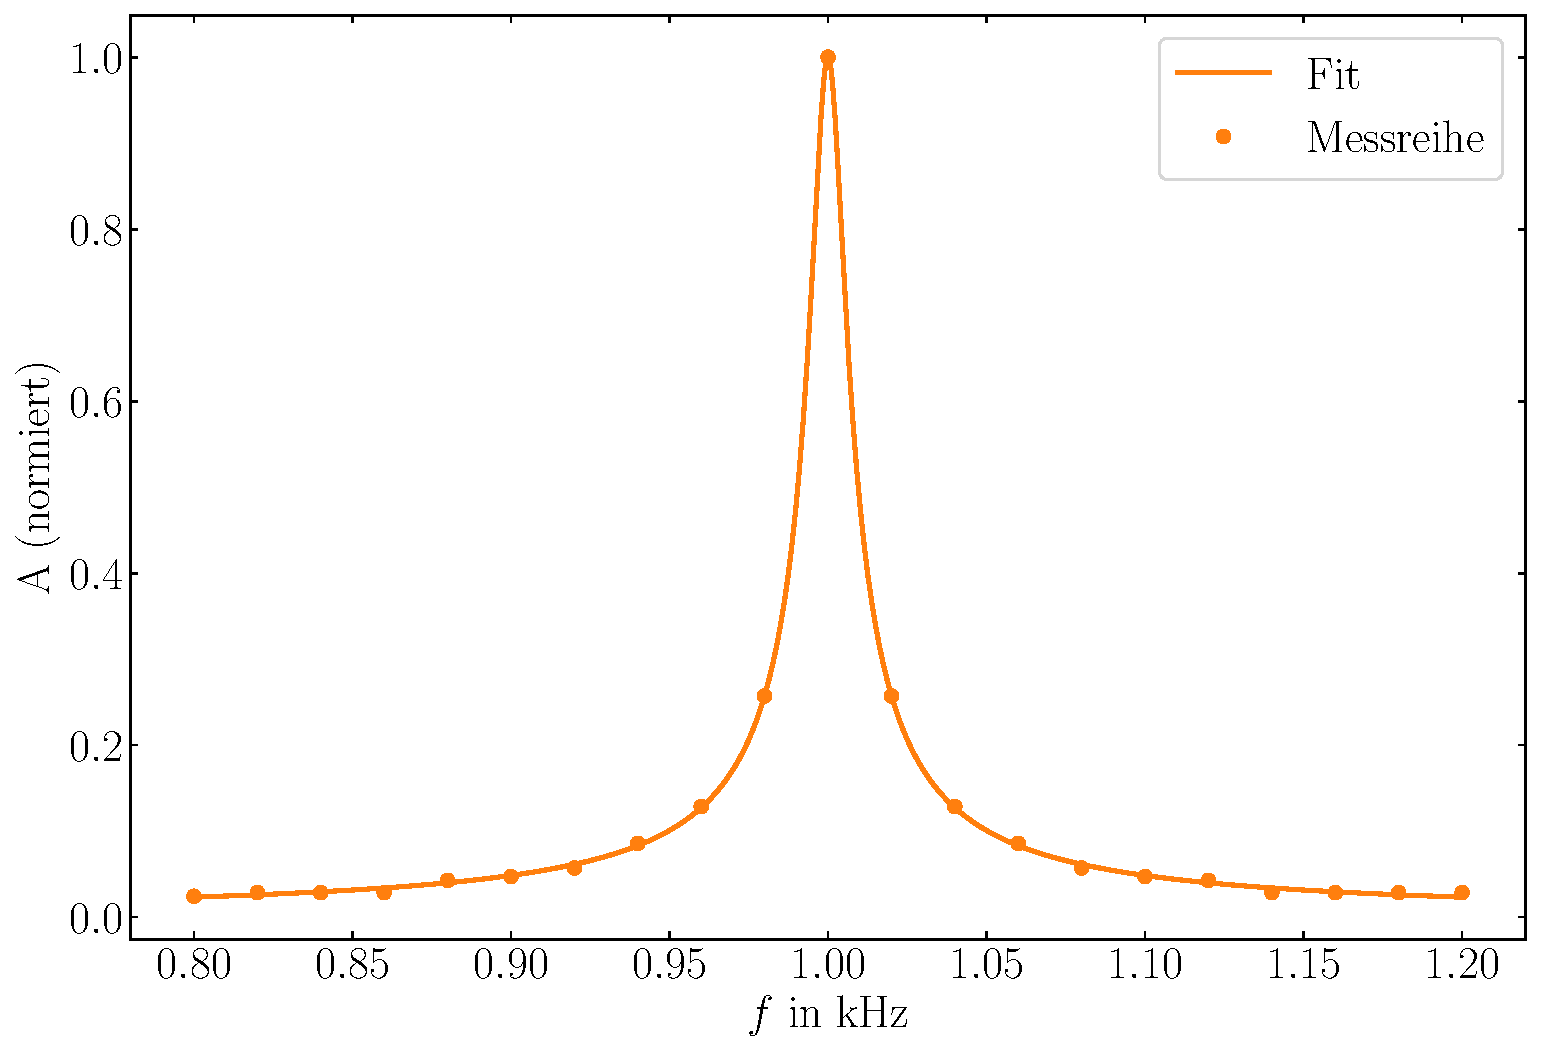
\includegraphics[scale = 0.5]{Manuel/44/6dB.pdf}
    \captionof{figure}{Fit für die Messung mit $\Delta$=6\,dB}
    \label{image:6dB}
    \vspace{1cm}
    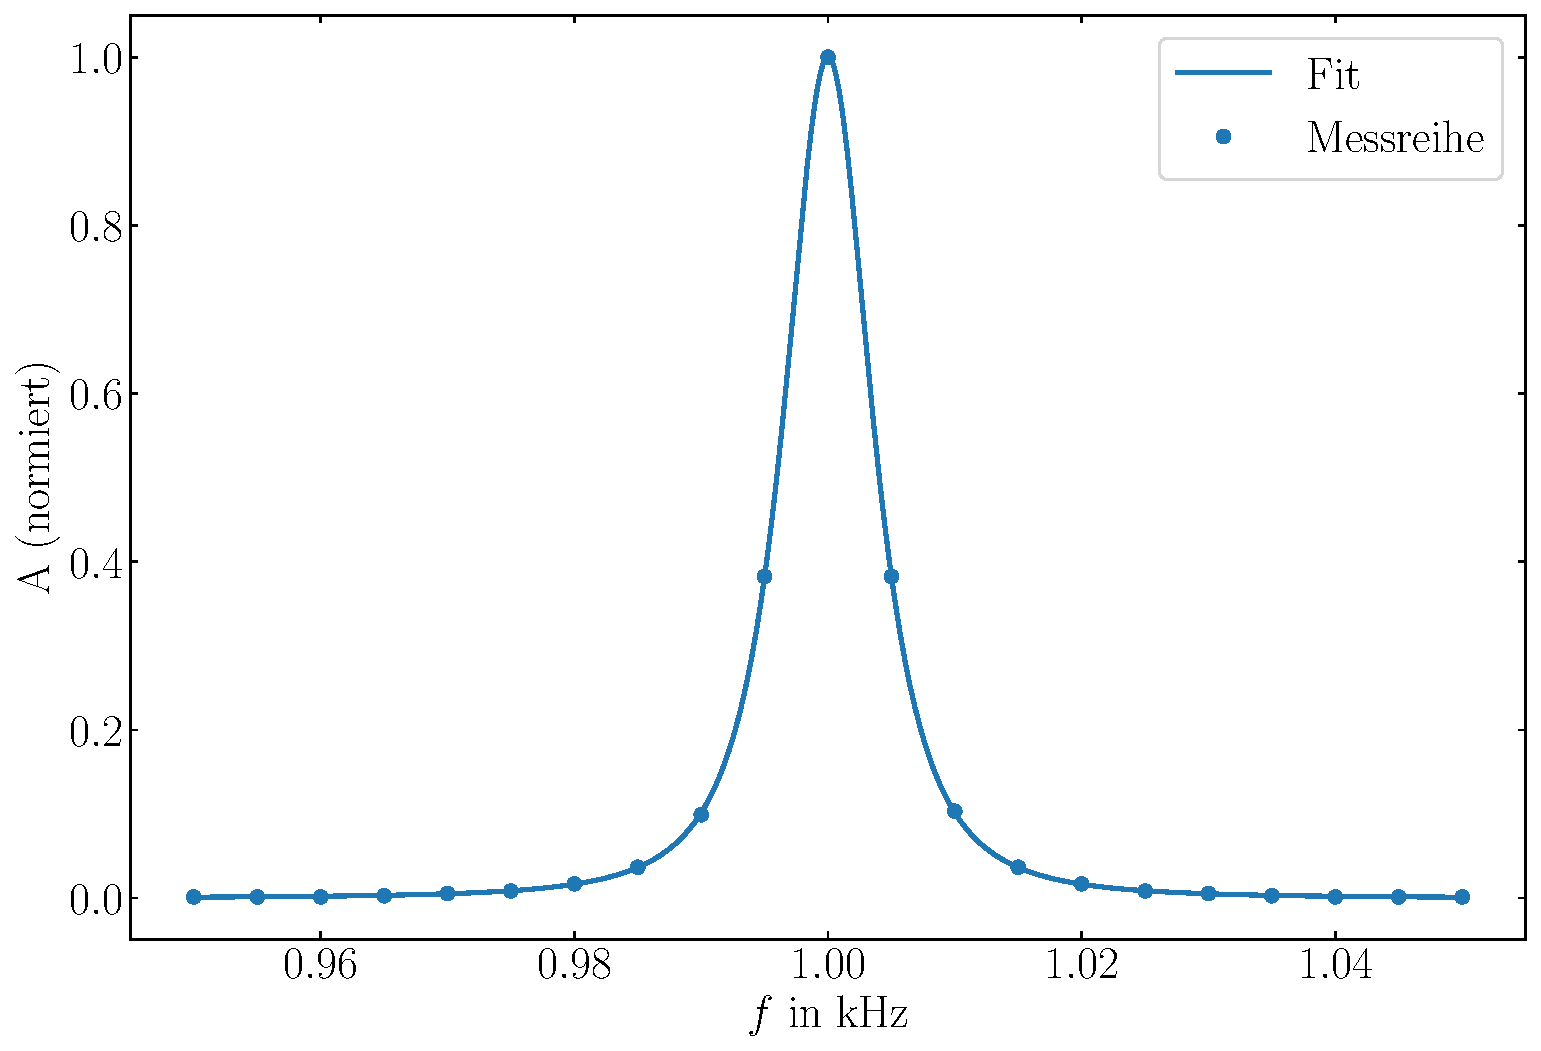
\includegraphics[scale = 0.5]{Manuel/44/18dB.pdf}
    \captionof{figure}{Fit für die Messung mit $\Delta$=18\,dB}
    \label{image:18dB}
    \vspace{1cm}
    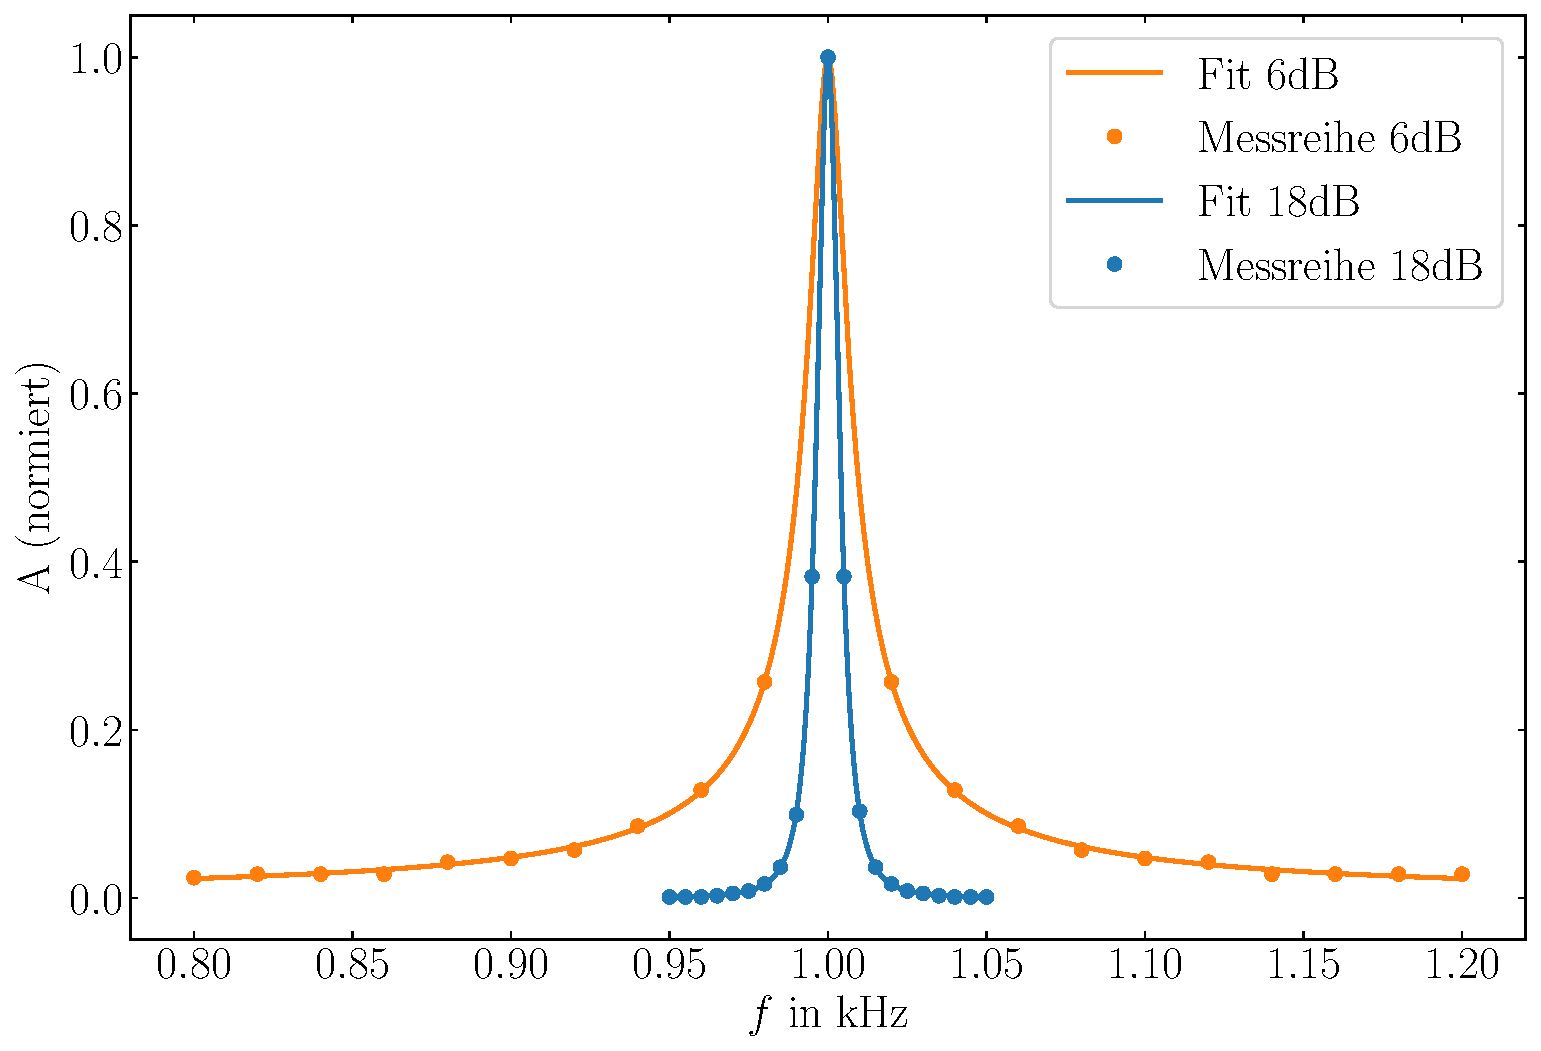
\includegraphics[scale = 0.5]{Manuel/44/All.pdf}
    \captionof{figure}{Vergleich beider Messreihen mit Fit}
    \label{image:All}
\end{center}

\paragraph{c)}\textbf{Lock-In in Praxis}

Im letzten Abschnitt wird noch die Verwendung eines Lock-In Verstärkers in der Praxis besprochen. Dazu stand eine Leuchtdiode und eine Photodiode in einer Box mit Deckel zur Verfügung. Die Signale von Leuchtdiode und Photodiode wurden dann auf dem Oszilloskop betrachtet. Man konnte beobachten, dass bei offenen Deckel große Schwankungen am Oszilloskop entstanden. Dies kann damit erklärt werden, das die Photodiode neben dem Signal der Leuchtdiode auch das Licht der Beleuchtung des Raums registriert hat, welches mit 50\,Hz flackert. Wurde der Deckel geschlossen, ließen die Schwankung nach und die Photodiode detektierte nur noch das Signal der Leuchtdiode, welches trotzdem sehr verrauscht war (zu sehen in Abb. \ref{image:oszi}). 

Die Änderung der Zeitkonstante $\tau$ und Flankensteilheit $\Delta$ am Lock-In Verstärker ergaben eine Veränderung der Auflösung des Lock-In Verstärkers. Dabei war die Auflösung am höchsten, wenn auch die Zeitkonstante und Flankensteilheit am höchsten waren.

%Die Bandbreite des Lock in Verstärkers lässt sich über die Grenzfrequenz $f_g$ bestimmen. Diese ist proportional zu $\frac{1}{\tau}$. In der Messung ist $\tau = 1$\,s (aus Abb. \ref{image:lockIn}), womit $f_g\approx 1$\,Hz ist, was der Bandbreite des Lock-In Verstärkers entspricht. Um diese Größe in dB umzurechnen, wird eine Referenzfrequenz benötigt, welche nicht beim Versuch aufgezeichnet wurde.

Die Detektionsbandbreite $B$ des Lock-In Verstärkers lässt sich wie folgt berechnen:
\begin{gather}
    B = 20\log_{10}\left(\frac{U_{min}}{U_{max}}\right)
\end{gather}
Bei dem verwendeten Loch-In Verstärker ist die maximale Spannung $U_{max}=$ 1\,V, was durch Bauart des Gerätes bedingt ist, und die minimal Spannung $U_{min} =$ 255\,nV. Damit ergibt sich eine Detektionsbreite $B =$ -132\,dB.

    % 5.Kapitel Fazit
    % 5. Einleitung

\chapter{Fazit}
\label{chap:fazit}
Alles in allem haben wir in diesem Versuch die Grundlagen der Rasterelektronenmikroskopie erlernen und anwenden dürfen. Dazu gehören die verschiedenen Detektoren und Einstellungsmöglichkeiten sowie die qualitative Analyse der aufgenommenen Bilder.\\
Unser gesammeltes Wissen wurde durch das ermitteln der Bruchursache nochmal gut gefestigt und uns wurde der Nutzen einer solchen Analyse in der Industrie klar deutlich. Auch wurde uns der Umgang mit biologischen Proben in diesem Versuch nahe gebracht, was uns in näherer Zukunft bestimmt zu gute kommen wird. Weiterhin finden wir es faszinierenden wie viel Struktur in einer so kleinen Welt noch zu finden ist und sin auch sehr überrascht, wie genau die Produktion eines Micro-Chips sein muss, um die Fertigung solch kleiner Schaltkreise zu ermöglichen.\\

Abschließen ist zu bemerken, dass der Versuch als Erfolg zu verbuchen ist, da er uns Praxisnah den Umgang mit einer der wichtigsten Untersuchungsmethoden vertraut gemacht hat.

    % Anhang
    %\chapter{Gemessene Plots}
\section{Tetrachlormethan}
\begin{figure}[h]
    \centering\subfigure[Stokes Linien]{\scalebox{0.9}{% GNUPLOT: LaTeX picture with Postscript
\begingroup
  % Encoding inside the plot.  In the header of your document, this encoding
  % should to defined, e.g., by using
  % \usepackage[cp1252,<other encodings>]{inputenc}
  \inputencoding{cp1252}%
  \makeatletter
  \providecommand\color[2][]{%
    \GenericError{(gnuplot) \space\space\space\@spaces}{%
      Package color not loaded in conjunction with
      terminal option `colourtext'%
    }{See the gnuplot documentation for explanation.%
    }{Either use 'blacktext' in gnuplot or load the package
      color.sty in LaTeX.}%
    \renewcommand\color[2][]{}%
  }%
  \providecommand\includegraphics[2][]{%
    \GenericError{(gnuplot) \space\space\space\@spaces}{%
      Package graphicx or graphics not loaded%
    }{See the gnuplot documentation for explanation.%
    }{The gnuplot epslatex terminal needs graphicx.sty or graphics.sty.}%
    \renewcommand\includegraphics[2][]{}%
  }%
  \providecommand\rotatebox[2]{#2}%
  \@ifundefined{ifGPcolor}{%
    \newif\ifGPcolor
    \GPcolorfalse
  }{}%
  \@ifundefined{ifGPblacktext}{%
    \newif\ifGPblacktext
    \GPblacktexttrue
  }{}%
  % define a \g@addto@macro without @ in the name:
  \let\gplgaddtomacro\g@addto@macro
  % define empty templates for all commands taking text:
  \gdef\gplbacktext{}%
  \gdef\gplfronttext{}%
  \makeatother
  \ifGPblacktext
    % no textcolor at all
    \def\colorrgb#1{}%
    \def\colorgray#1{}%
  \else
    % gray or color?
    \ifGPcolor
      \def\colorrgb#1{\color[rgb]{#1}}%
      \def\colorgray#1{\color[gray]{#1}}%
      \expandafter\def\csname LTw\endcsname{\color{white}}%
      \expandafter\def\csname LTb\endcsname{\color{black}}%
      \expandafter\def\csname LTa\endcsname{\color{black}}%
      \expandafter\def\csname LT0\endcsname{\color[rgb]{1,0,0}}%
      \expandafter\def\csname LT1\endcsname{\color[rgb]{0,1,0}}%
      \expandafter\def\csname LT2\endcsname{\color[rgb]{0,0,1}}%
      \expandafter\def\csname LT3\endcsname{\color[rgb]{1,0,1}}%
      \expandafter\def\csname LT4\endcsname{\color[rgb]{0,1,1}}%
      \expandafter\def\csname LT5\endcsname{\color[rgb]{1,1,0}}%
      \expandafter\def\csname LT6\endcsname{\color[rgb]{0,0,0}}%
      \expandafter\def\csname LT7\endcsname{\color[rgb]{1,0.3,0}}%
      \expandafter\def\csname LT8\endcsname{\color[rgb]{0.5,0.5,0.5}}%
    \else
      % gray
      \def\colorrgb#1{\color{black}}%
      \def\colorgray#1{\color[gray]{#1}}%
      \expandafter\def\csname LTw\endcsname{\color{white}}%
      \expandafter\def\csname LTb\endcsname{\color{black}}%
      \expandafter\def\csname LTa\endcsname{\color{black}}%
      \expandafter\def\csname LT0\endcsname{\color{black}}%
      \expandafter\def\csname LT1\endcsname{\color{black}}%
      \expandafter\def\csname LT2\endcsname{\color{black}}%
      \expandafter\def\csname LT3\endcsname{\color{black}}%
      \expandafter\def\csname LT4\endcsname{\color{black}}%
      \expandafter\def\csname LT5\endcsname{\color{black}}%
      \expandafter\def\csname LT6\endcsname{\color{black}}%
      \expandafter\def\csname LT7\endcsname{\color{black}}%
      \expandafter\def\csname LT8\endcsname{\color{black}}%
    \fi
  \fi
    \setlength{\unitlength}{0.0500bp}%
    \ifx\gptboxheight\undefined%
      \newlength{\gptboxheight}%
      \newlength{\gptboxwidth}%
      \newsavebox{\gptboxtext}%
    \fi%
    \setlength{\fboxrule}{0.5pt}%
    \setlength{\fboxsep}{1pt}%
\begin{picture}(7200.00,5040.00)%
    \gplgaddtomacro\gplbacktext{%
      \csname LTb\endcsname%%
      \put(726,440){\makebox(0,0)[r]{\strut{}$0.05$}}%
      \put(726,1316){\makebox(0,0)[r]{\strut{}$0.1$}}%
      \put(726,2192){\makebox(0,0)[r]{\strut{}$0.15$}}%
      \put(726,3067){\makebox(0,0)[r]{\strut{}$0.2$}}%
      \put(726,3943){\makebox(0,0)[r]{\strut{}$0.25$}}%
      \put(726,4819){\makebox(0,0)[r]{\strut{}$0.3$}}%
      \put(858,220){\makebox(0,0){\strut{}$560$}}%
      \put(1601,220){\makebox(0,0){\strut{}$570$}}%
      \put(2344,220){\makebox(0,0){\strut{}$580$}}%
      \put(3087,220){\makebox(0,0){\strut{}$590$}}%
      \put(3831,220){\makebox(0,0){\strut{}$600$}}%
      \put(4574,220){\makebox(0,0){\strut{}$610$}}%
      \put(5317,220){\makebox(0,0){\strut{}$620$}}%
      \put(6060,220){\makebox(0,0){\strut{}$630$}}%
      \put(6803,220){\makebox(0,0){\strut{}$640$}}%
    }%
    \gplgaddtomacro\gplfronttext{%
      \csname LTb\endcsname%%
      \put(3102,4646){\makebox(0,0)[r]{\strut{}$0^\circ$ Polarisation}}%
      \csname LTb\endcsname%%
      \put(3102,4426){\makebox(0,0)[r]{\strut{}$90^\circ$ Polarisation}}%
    }%
    \gplbacktext
    \put(0,0){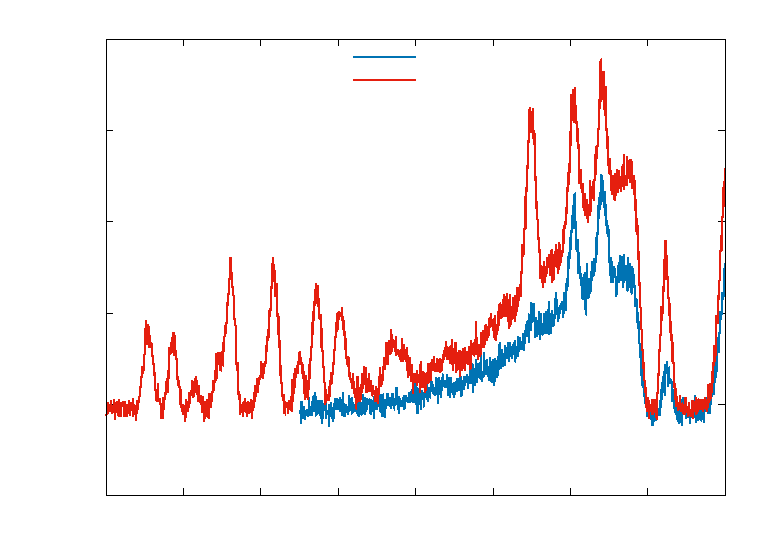
\includegraphics[width={360.00bp},height={252.00bp}]{Anhang/ccl4_s}}%
    \gplfronttext
  \end{picture}%
\endgroup
}}\\
    \subfigure[Anti-Stokes Linien]{\scalebox{0.9}{% GNUPLOT: LaTeX picture with Postscript
\begingroup
  % Encoding inside the plot.  In the header of your document, this encoding
  % should to defined, e.g., by using
  % \usepackage[cp1252,<other encodings>]{inputenc}
  \inputencoding{cp1252}%
  \makeatletter
  \providecommand\color[2][]{%
    \GenericError{(gnuplot) \space\space\space\@spaces}{%
      Package color not loaded in conjunction with
      terminal option `colourtext'%
    }{See the gnuplot documentation for explanation.%
    }{Either use 'blacktext' in gnuplot or load the package
      color.sty in LaTeX.}%
    \renewcommand\color[2][]{}%
  }%
  \providecommand\includegraphics[2][]{%
    \GenericError{(gnuplot) \space\space\space\@spaces}{%
      Package graphicx or graphics not loaded%
    }{See the gnuplot documentation for explanation.%
    }{The gnuplot epslatex terminal needs graphicx.sty or graphics.sty.}%
    \renewcommand\includegraphics[2][]{}%
  }%
  \providecommand\rotatebox[2]{#2}%
  \@ifundefined{ifGPcolor}{%
    \newif\ifGPcolor
    \GPcolorfalse
  }{}%
  \@ifundefined{ifGPblacktext}{%
    \newif\ifGPblacktext
    \GPblacktexttrue
  }{}%
  % define a \g@addto@macro without @ in the name:
  \let\gplgaddtomacro\g@addto@macro
  % define empty templates for all commands taking text:
  \gdef\gplbacktext{}%
  \gdef\gplfronttext{}%
  \makeatother
  \ifGPblacktext
    % no textcolor at all
    \def\colorrgb#1{}%
    \def\colorgray#1{}%
  \else
    % gray or color?
    \ifGPcolor
      \def\colorrgb#1{\color[rgb]{#1}}%
      \def\colorgray#1{\color[gray]{#1}}%
      \expandafter\def\csname LTw\endcsname{\color{white}}%
      \expandafter\def\csname LTb\endcsname{\color{black}}%
      \expandafter\def\csname LTa\endcsname{\color{black}}%
      \expandafter\def\csname LT0\endcsname{\color[rgb]{1,0,0}}%
      \expandafter\def\csname LT1\endcsname{\color[rgb]{0,1,0}}%
      \expandafter\def\csname LT2\endcsname{\color[rgb]{0,0,1}}%
      \expandafter\def\csname LT3\endcsname{\color[rgb]{1,0,1}}%
      \expandafter\def\csname LT4\endcsname{\color[rgb]{0,1,1}}%
      \expandafter\def\csname LT5\endcsname{\color[rgb]{1,1,0}}%
      \expandafter\def\csname LT6\endcsname{\color[rgb]{0,0,0}}%
      \expandafter\def\csname LT7\endcsname{\color[rgb]{1,0.3,0}}%
      \expandafter\def\csname LT8\endcsname{\color[rgb]{0.5,0.5,0.5}}%
    \else
      % gray
      \def\colorrgb#1{\color{black}}%
      \def\colorgray#1{\color[gray]{#1}}%
      \expandafter\def\csname LTw\endcsname{\color{white}}%
      \expandafter\def\csname LTb\endcsname{\color{black}}%
      \expandafter\def\csname LTa\endcsname{\color{black}}%
      \expandafter\def\csname LT0\endcsname{\color{black}}%
      \expandafter\def\csname LT1\endcsname{\color{black}}%
      \expandafter\def\csname LT2\endcsname{\color{black}}%
      \expandafter\def\csname LT3\endcsname{\color{black}}%
      \expandafter\def\csname LT4\endcsname{\color{black}}%
      \expandafter\def\csname LT5\endcsname{\color{black}}%
      \expandafter\def\csname LT6\endcsname{\color{black}}%
      \expandafter\def\csname LT7\endcsname{\color{black}}%
      \expandafter\def\csname LT8\endcsname{\color{black}}%
    \fi
  \fi
    \setlength{\unitlength}{0.0500bp}%
    \ifx\gptboxheight\undefined%
      \newlength{\gptboxheight}%
      \newlength{\gptboxwidth}%
      \newsavebox{\gptboxtext}%
    \fi%
    \setlength{\fboxrule}{0.5pt}%
    \setlength{\fboxsep}{1pt}%
\begin{picture}(7200.00,5040.00)%
    \gplgaddtomacro\gplbacktext{%
      \csname LTb\endcsname%%
      \put(594,440){\makebox(0,0)[r]{\strut{}$0$}}%
      \put(594,987){\makebox(0,0)[r]{\strut{}$0.1$}}%
      \put(594,1535){\makebox(0,0)[r]{\strut{}$0.2$}}%
      \put(594,2082){\makebox(0,0)[r]{\strut{}$0.3$}}%
      \put(594,2630){\makebox(0,0)[r]{\strut{}$0.4$}}%
      \put(594,3177){\makebox(0,0)[r]{\strut{}$0.5$}}%
      \put(594,3724){\makebox(0,0)[r]{\strut{}$0.6$}}%
      \put(594,4272){\makebox(0,0)[r]{\strut{}$0.7$}}%
      \put(594,4819){\makebox(0,0)[r]{\strut{}$0.8$}}%
      \put(726,220){\makebox(0,0){\strut{}$625$}}%
      \put(1334,220){\makebox(0,0){\strut{}$630$}}%
      \put(1941,220){\makebox(0,0){\strut{}$635$}}%
      \put(2549,220){\makebox(0,0){\strut{}$640$}}%
      \put(3157,220){\makebox(0,0){\strut{}$645$}}%
      \put(3765,220){\makebox(0,0){\strut{}$650$}}%
      \put(4372,220){\makebox(0,0){\strut{}$655$}}%
      \put(4980,220){\makebox(0,0){\strut{}$660$}}%
      \put(5588,220){\makebox(0,0){\strut{}$665$}}%
      \put(6195,220){\makebox(0,0){\strut{}$670$}}%
      \put(6803,220){\makebox(0,0){\strut{}$675$}}%
    }%
    \gplgaddtomacro\gplfronttext{%
      \csname LTb\endcsname%%
      \put(2970,4646){\makebox(0,0)[r]{\strut{}$0^\circ$ Polarisation}}%
      \csname LTb\endcsname%%
      \put(2970,4426){\makebox(0,0)[r]{\strut{}$90^\circ$ Polarisation}}%
    }%
    \gplbacktext
    \put(0,0){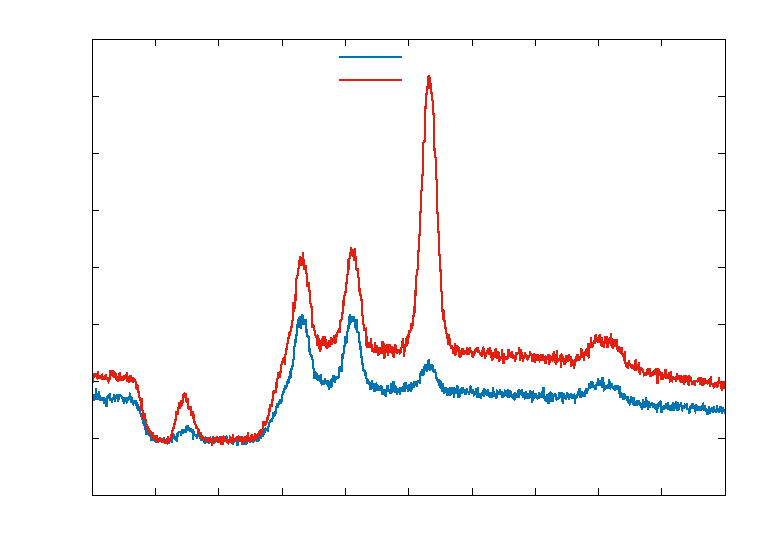
\includegraphics[width={360.00bp},height={252.00bp}]{Anhang/ccl4_as}}%
    \gplfronttext
  \end{picture}%
\endgroup
}}
    \caption{Gemessene Plots für Tetrachlormethan für $0^\circ$ und $90^\circ$-Polarisation im (Anti-)Stokes-Bereich}
\end{figure}\newpage
\section{Chlorophorm}
\begin{figure}[h]
    \centering\subfigure[Stokes Linien]{\scalebox{0.94}{% GNUPLOT: LaTeX picture with Postscript
\begingroup
  % Encoding inside the plot.  In the header of your document, this encoding
  % should to defined, e.g., by using
  % \usepackage[cp1252,<other encodings>]{inputenc}
  \inputencoding{cp1252}%
  \makeatletter
  \providecommand\color[2][]{%
    \GenericError{(gnuplot) \space\space\space\@spaces}{%
      Package color not loaded in conjunction with
      terminal option `colourtext'%
    }{See the gnuplot documentation for explanation.%
    }{Either use 'blacktext' in gnuplot or load the package
      color.sty in LaTeX.}%
    \renewcommand\color[2][]{}%
  }%
  \providecommand\includegraphics[2][]{%
    \GenericError{(gnuplot) \space\space\space\@spaces}{%
      Package graphicx or graphics not loaded%
    }{See the gnuplot documentation for explanation.%
    }{The gnuplot epslatex terminal needs graphicx.sty or graphics.sty.}%
    \renewcommand\includegraphics[2][]{}%
  }%
  \providecommand\rotatebox[2]{#2}%
  \@ifundefined{ifGPcolor}{%
    \newif\ifGPcolor
    \GPcolorfalse
  }{}%
  \@ifundefined{ifGPblacktext}{%
    \newif\ifGPblacktext
    \GPblacktexttrue
  }{}%
  % define a \g@addto@macro without @ in the name:
  \let\gplgaddtomacro\g@addto@macro
  % define empty templates for all commands taking text:
  \gdef\gplbacktext{}%
  \gdef\gplfronttext{}%
  \makeatother
  \ifGPblacktext
    % no textcolor at all
    \def\colorrgb#1{}%
    \def\colorgray#1{}%
  \else
    % gray or color?
    \ifGPcolor
      \def\colorrgb#1{\color[rgb]{#1}}%
      \def\colorgray#1{\color[gray]{#1}}%
      \expandafter\def\csname LTw\endcsname{\color{white}}%
      \expandafter\def\csname LTb\endcsname{\color{black}}%
      \expandafter\def\csname LTa\endcsname{\color{black}}%
      \expandafter\def\csname LT0\endcsname{\color[rgb]{1,0,0}}%
      \expandafter\def\csname LT1\endcsname{\color[rgb]{0,1,0}}%
      \expandafter\def\csname LT2\endcsname{\color[rgb]{0,0,1}}%
      \expandafter\def\csname LT3\endcsname{\color[rgb]{1,0,1}}%
      \expandafter\def\csname LT4\endcsname{\color[rgb]{0,1,1}}%
      \expandafter\def\csname LT5\endcsname{\color[rgb]{1,1,0}}%
      \expandafter\def\csname LT6\endcsname{\color[rgb]{0,0,0}}%
      \expandafter\def\csname LT7\endcsname{\color[rgb]{1,0.3,0}}%
      \expandafter\def\csname LT8\endcsname{\color[rgb]{0.5,0.5,0.5}}%
    \else
      % gray
      \def\colorrgb#1{\color{black}}%
      \def\colorgray#1{\color[gray]{#1}}%
      \expandafter\def\csname LTw\endcsname{\color{white}}%
      \expandafter\def\csname LTb\endcsname{\color{black}}%
      \expandafter\def\csname LTa\endcsname{\color{black}}%
      \expandafter\def\csname LT0\endcsname{\color{black}}%
      \expandafter\def\csname LT1\endcsname{\color{black}}%
      \expandafter\def\csname LT2\endcsname{\color{black}}%
      \expandafter\def\csname LT3\endcsname{\color{black}}%
      \expandafter\def\csname LT4\endcsname{\color{black}}%
      \expandafter\def\csname LT5\endcsname{\color{black}}%
      \expandafter\def\csname LT6\endcsname{\color{black}}%
      \expandafter\def\csname LT7\endcsname{\color{black}}%
      \expandafter\def\csname LT8\endcsname{\color{black}}%
    \fi
  \fi
    \setlength{\unitlength}{0.0500bp}%
    \ifx\gptboxheight\undefined%
      \newlength{\gptboxheight}%
      \newlength{\gptboxwidth}%
      \newsavebox{\gptboxtext}%
    \fi%
    \setlength{\fboxrule}{0.5pt}%
    \setlength{\fboxsep}{1pt}%
\begin{picture}(7200.00,5040.00)%
    \gplgaddtomacro\gplbacktext{%
      \csname LTb\endcsname%%
      \put(726,440){\makebox(0,0)[r]{\strut{}$0.08$}}%
      \put(726,1170){\makebox(0,0)[r]{\strut{}$0.1$}}%
      \put(726,1900){\makebox(0,0)[r]{\strut{}$0.12$}}%
      \put(726,2629){\makebox(0,0)[r]{\strut{}$0.14$}}%
      \put(726,3359){\makebox(0,0)[r]{\strut{}$0.16$}}%
      \put(726,4089){\makebox(0,0)[r]{\strut{}$0.18$}}%
      \put(726,4819){\makebox(0,0)[r]{\strut{}$0.2$}}%
      \put(858,220){\makebox(0,0){\strut{}$560$}}%
      \put(1601,220){\makebox(0,0){\strut{}$570$}}%
      \put(2344,220){\makebox(0,0){\strut{}$580$}}%
      \put(3087,220){\makebox(0,0){\strut{}$590$}}%
      \put(3831,220){\makebox(0,0){\strut{}$600$}}%
      \put(4574,220){\makebox(0,0){\strut{}$610$}}%
      \put(5317,220){\makebox(0,0){\strut{}$620$}}%
      \put(6060,220){\makebox(0,0){\strut{}$630$}}%
      \put(6803,220){\makebox(0,0){\strut{}$640$}}%
    }%
    \gplgaddtomacro\gplfronttext{%
      \csname LTb\endcsname%%
      \put(3102,4646){\makebox(0,0)[r]{\strut{}$0^\circ$ Polarisation}}%
      \csname LTb\endcsname%%
      \put(3102,4426){\makebox(0,0)[r]{\strut{}$90^\circ$ Polarisation}}%
    }%
    \gplbacktext
    \put(0,0){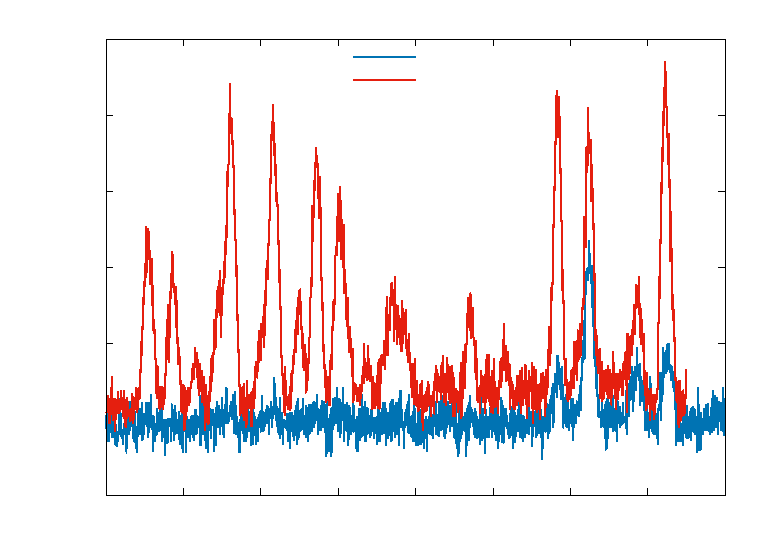
\includegraphics[width={360.00bp},height={252.00bp}]{Anhang/chcl3_s}}%
    \gplfronttext
  \end{picture}%
\endgroup
}}\\
    \subfigure[Anti-Stokes Linien]{\scalebox{0.94}{% GNUPLOT: LaTeX picture with Postscript
\begingroup
  % Encoding inside the plot.  In the header of your document, this encoding
  % should to defined, e.g., by using
  % \usepackage[cp1252,<other encodings>]{inputenc}
  \inputencoding{cp1252}%
  \makeatletter
  \providecommand\color[2][]{%
    \GenericError{(gnuplot) \space\space\space\@spaces}{%
      Package color not loaded in conjunction with
      terminal option `colourtext'%
    }{See the gnuplot documentation for explanation.%
    }{Either use 'blacktext' in gnuplot or load the package
      color.sty in LaTeX.}%
    \renewcommand\color[2][]{}%
  }%
  \providecommand\includegraphics[2][]{%
    \GenericError{(gnuplot) \space\space\space\@spaces}{%
      Package graphicx or graphics not loaded%
    }{See the gnuplot documentation for explanation.%
    }{The gnuplot epslatex terminal needs graphicx.sty or graphics.sty.}%
    \renewcommand\includegraphics[2][]{}%
  }%
  \providecommand\rotatebox[2]{#2}%
  \@ifundefined{ifGPcolor}{%
    \newif\ifGPcolor
    \GPcolorfalse
  }{}%
  \@ifundefined{ifGPblacktext}{%
    \newif\ifGPblacktext
    \GPblacktexttrue
  }{}%
  % define a \g@addto@macro without @ in the name:
  \let\gplgaddtomacro\g@addto@macro
  % define empty templates for all commands taking text:
  \gdef\gplbacktext{}%
  \gdef\gplfronttext{}%
  \makeatother
  \ifGPblacktext
    % no textcolor at all
    \def\colorrgb#1{}%
    \def\colorgray#1{}%
  \else
    % gray or color?
    \ifGPcolor
      \def\colorrgb#1{\color[rgb]{#1}}%
      \def\colorgray#1{\color[gray]{#1}}%
      \expandafter\def\csname LTw\endcsname{\color{white}}%
      \expandafter\def\csname LTb\endcsname{\color{black}}%
      \expandafter\def\csname LTa\endcsname{\color{black}}%
      \expandafter\def\csname LT0\endcsname{\color[rgb]{1,0,0}}%
      \expandafter\def\csname LT1\endcsname{\color[rgb]{0,1,0}}%
      \expandafter\def\csname LT2\endcsname{\color[rgb]{0,0,1}}%
      \expandafter\def\csname LT3\endcsname{\color[rgb]{1,0,1}}%
      \expandafter\def\csname LT4\endcsname{\color[rgb]{0,1,1}}%
      \expandafter\def\csname LT5\endcsname{\color[rgb]{1,1,0}}%
      \expandafter\def\csname LT6\endcsname{\color[rgb]{0,0,0}}%
      \expandafter\def\csname LT7\endcsname{\color[rgb]{1,0.3,0}}%
      \expandafter\def\csname LT8\endcsname{\color[rgb]{0.5,0.5,0.5}}%
    \else
      % gray
      \def\colorrgb#1{\color{black}}%
      \def\colorgray#1{\color[gray]{#1}}%
      \expandafter\def\csname LTw\endcsname{\color{white}}%
      \expandafter\def\csname LTb\endcsname{\color{black}}%
      \expandafter\def\csname LTa\endcsname{\color{black}}%
      \expandafter\def\csname LT0\endcsname{\color{black}}%
      \expandafter\def\csname LT1\endcsname{\color{black}}%
      \expandafter\def\csname LT2\endcsname{\color{black}}%
      \expandafter\def\csname LT3\endcsname{\color{black}}%
      \expandafter\def\csname LT4\endcsname{\color{black}}%
      \expandafter\def\csname LT5\endcsname{\color{black}}%
      \expandafter\def\csname LT6\endcsname{\color{black}}%
      \expandafter\def\csname LT7\endcsname{\color{black}}%
      \expandafter\def\csname LT8\endcsname{\color{black}}%
    \fi
  \fi
    \setlength{\unitlength}{0.0500bp}%
    \ifx\gptboxheight\undefined%
      \newlength{\gptboxheight}%
      \newlength{\gptboxwidth}%
      \newsavebox{\gptboxtext}%
    \fi%
    \setlength{\fboxrule}{0.5pt}%
    \setlength{\fboxsep}{1pt}%
\begin{picture}(7200.00,5040.00)%
    \gplgaddtomacro\gplbacktext{%
      \csname LTb\endcsname%%
      \put(726,440){\makebox(0,0)[r]{\strut{}$0.05$}}%
      \put(726,1066){\makebox(0,0)[r]{\strut{}$0.1$}}%
      \put(726,1691){\makebox(0,0)[r]{\strut{}$0.15$}}%
      \put(726,2317){\makebox(0,0)[r]{\strut{}$0.2$}}%
      \put(726,2942){\makebox(0,0)[r]{\strut{}$0.25$}}%
      \put(726,3568){\makebox(0,0)[r]{\strut{}$0.3$}}%
      \put(726,4193){\makebox(0,0)[r]{\strut{}$0.35$}}%
      \put(726,4819){\makebox(0,0)[r]{\strut{}$0.4$}}%
      \put(858,220){\makebox(0,0){\strut{}$620$}}%
      \put(1707,220){\makebox(0,0){\strut{}$630$}}%
      \put(2557,220){\makebox(0,0){\strut{}$640$}}%
      \put(3406,220){\makebox(0,0){\strut{}$650$}}%
      \put(4255,220){\makebox(0,0){\strut{}$660$}}%
      \put(5104,220){\makebox(0,0){\strut{}$670$}}%
      \put(5954,220){\makebox(0,0){\strut{}$680$}}%
      \put(6803,220){\makebox(0,0){\strut{}$690$}}%
    }%
    \gplgaddtomacro\gplfronttext{%
      \csname LTb\endcsname%%
      \put(3102,4646){\makebox(0,0)[r]{\strut{}$0^\circ$ Polarisation}}%
      \csname LTb\endcsname%%
      \put(3102,4426){\makebox(0,0)[r]{\strut{}$90^\circ$ Polarisation}}%
    }%
    \gplbacktext
    \put(0,0){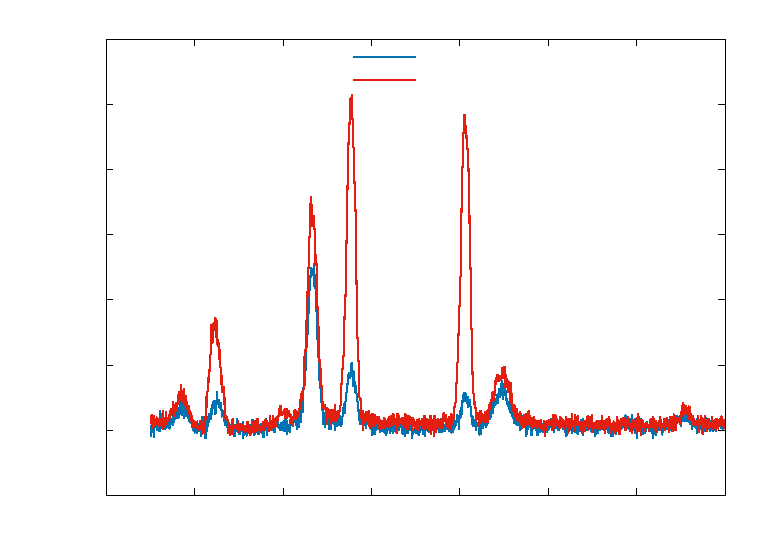
\includegraphics[width={360.00bp},height={252.00bp}]{Anhang/chcl3_as}}%
    \gplfronttext
  \end{picture}%
\endgroup
}}
    \caption{Gemessene Plots für Chlorophorm für $0^\circ$ und $90^\circ$-Polarisation im (Anti-)Stokes-Bereich}
\end{figure}\newpage
\section{Deuterium Chlorophorm}
\begin{figure}[h]
    \centering\subfigure[Stokes Linien]{\scalebox{0.94}{% GNUPLOT: LaTeX picture with Postscript
\begingroup
  % Encoding inside the plot.  In the header of your document, this encoding
  % should to defined, e.g., by using
  % \usepackage[cp1252,<other encodings>]{inputenc}
  \inputencoding{cp1252}%
  \makeatletter
  \providecommand\color[2][]{%
    \GenericError{(gnuplot) \space\space\space\@spaces}{%
      Package color not loaded in conjunction with
      terminal option `colourtext'%
    }{See the gnuplot documentation for explanation.%
    }{Either use 'blacktext' in gnuplot or load the package
      color.sty in LaTeX.}%
    \renewcommand\color[2][]{}%
  }%
  \providecommand\includegraphics[2][]{%
    \GenericError{(gnuplot) \space\space\space\@spaces}{%
      Package graphicx or graphics not loaded%
    }{See the gnuplot documentation for explanation.%
    }{The gnuplot epslatex terminal needs graphicx.sty or graphics.sty.}%
    \renewcommand\includegraphics[2][]{}%
  }%
  \providecommand\rotatebox[2]{#2}%
  \@ifundefined{ifGPcolor}{%
    \newif\ifGPcolor
    \GPcolorfalse
  }{}%
  \@ifundefined{ifGPblacktext}{%
    \newif\ifGPblacktext
    \GPblacktexttrue
  }{}%
  % define a \g@addto@macro without @ in the name:
  \let\gplgaddtomacro\g@addto@macro
  % define empty templates for all commands taking text:
  \gdef\gplbacktext{}%
  \gdef\gplfronttext{}%
  \makeatother
  \ifGPblacktext
    % no textcolor at all
    \def\colorrgb#1{}%
    \def\colorgray#1{}%
  \else
    % gray or color?
    \ifGPcolor
      \def\colorrgb#1{\color[rgb]{#1}}%
      \def\colorgray#1{\color[gray]{#1}}%
      \expandafter\def\csname LTw\endcsname{\color{white}}%
      \expandafter\def\csname LTb\endcsname{\color{black}}%
      \expandafter\def\csname LTa\endcsname{\color{black}}%
      \expandafter\def\csname LT0\endcsname{\color[rgb]{1,0,0}}%
      \expandafter\def\csname LT1\endcsname{\color[rgb]{0,1,0}}%
      \expandafter\def\csname LT2\endcsname{\color[rgb]{0,0,1}}%
      \expandafter\def\csname LT3\endcsname{\color[rgb]{1,0,1}}%
      \expandafter\def\csname LT4\endcsname{\color[rgb]{0,1,1}}%
      \expandafter\def\csname LT5\endcsname{\color[rgb]{1,1,0}}%
      \expandafter\def\csname LT6\endcsname{\color[rgb]{0,0,0}}%
      \expandafter\def\csname LT7\endcsname{\color[rgb]{1,0.3,0}}%
      \expandafter\def\csname LT8\endcsname{\color[rgb]{0.5,0.5,0.5}}%
    \else
      % gray
      \def\colorrgb#1{\color{black}}%
      \def\colorgray#1{\color[gray]{#1}}%
      \expandafter\def\csname LTw\endcsname{\color{white}}%
      \expandafter\def\csname LTb\endcsname{\color{black}}%
      \expandafter\def\csname LTa\endcsname{\color{black}}%
      \expandafter\def\csname LT0\endcsname{\color{black}}%
      \expandafter\def\csname LT1\endcsname{\color{black}}%
      \expandafter\def\csname LT2\endcsname{\color{black}}%
      \expandafter\def\csname LT3\endcsname{\color{black}}%
      \expandafter\def\csname LT4\endcsname{\color{black}}%
      \expandafter\def\csname LT5\endcsname{\color{black}}%
      \expandafter\def\csname LT6\endcsname{\color{black}}%
      \expandafter\def\csname LT7\endcsname{\color{black}}%
      \expandafter\def\csname LT8\endcsname{\color{black}}%
    \fi
  \fi
    \setlength{\unitlength}{0.0500bp}%
    \ifx\gptboxheight\undefined%
      \newlength{\gptboxheight}%
      \newlength{\gptboxwidth}%
      \newsavebox{\gptboxtext}%
    \fi%
    \setlength{\fboxrule}{0.5pt}%
    \setlength{\fboxsep}{1pt}%
\begin{picture}(7200.00,5040.00)%
    \gplgaddtomacro\gplbacktext{%
      \csname LTb\endcsname%%
      \put(726,440){\makebox(0,0)[r]{\strut{}$0.06$}}%
      \put(726,1066){\makebox(0,0)[r]{\strut{}$0.08$}}%
      \put(726,1691){\makebox(0,0)[r]{\strut{}$0.1$}}%
      \put(726,2317){\makebox(0,0)[r]{\strut{}$0.12$}}%
      \put(726,2942){\makebox(0,0)[r]{\strut{}$0.14$}}%
      \put(726,3568){\makebox(0,0)[r]{\strut{}$0.16$}}%
      \put(726,4193){\makebox(0,0)[r]{\strut{}$0.18$}}%
      \put(726,4819){\makebox(0,0)[r]{\strut{}$0.2$}}%
      \put(858,220){\makebox(0,0){\strut{}$570$}}%
      \put(1707,220){\makebox(0,0){\strut{}$580$}}%
      \put(2557,220){\makebox(0,0){\strut{}$590$}}%
      \put(3406,220){\makebox(0,0){\strut{}$600$}}%
      \put(4255,220){\makebox(0,0){\strut{}$610$}}%
      \put(5104,220){\makebox(0,0){\strut{}$620$}}%
      \put(5954,220){\makebox(0,0){\strut{}$630$}}%
      \put(6803,220){\makebox(0,0){\strut{}$640$}}%
    }%
    \gplgaddtomacro\gplfronttext{%
      \csname LTb\endcsname%%
      \put(3102,4646){\makebox(0,0)[r]{\strut{}$0^\circ$ Polarisation}}%
      \csname LTb\endcsname%%
      \put(3102,4426){\makebox(0,0)[r]{\strut{}$90^\circ$ Polarisation}}%
    }%
    \gplbacktext
    \put(0,0){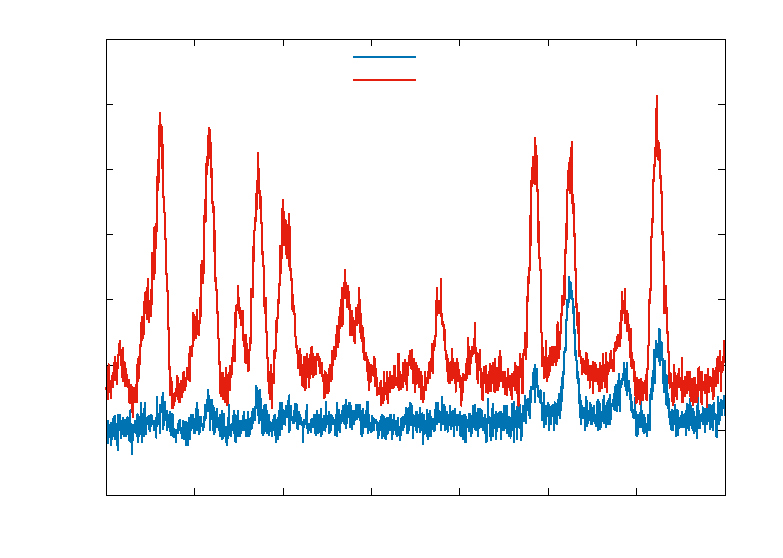
\includegraphics[width={360.00bp},height={252.00bp}]{Anhang/cdcl3_s}}%
    \gplfronttext
  \end{picture}%
\endgroup
}}\\
    \subfigure[Anti-Stokes Linien]{\scalebox{0.94}{% GNUPLOT: LaTeX picture with Postscript
\begingroup
  % Encoding inside the plot.  In the header of your document, this encoding
  % should to defined, e.g., by using
  % \usepackage[cp1252,<other encodings>]{inputenc}
  \inputencoding{cp1252}%
  \makeatletter
  \providecommand\color[2][]{%
    \GenericError{(gnuplot) \space\space\space\@spaces}{%
      Package color not loaded in conjunction with
      terminal option `colourtext'%
    }{See the gnuplot documentation for explanation.%
    }{Either use 'blacktext' in gnuplot or load the package
      color.sty in LaTeX.}%
    \renewcommand\color[2][]{}%
  }%
  \providecommand\includegraphics[2][]{%
    \GenericError{(gnuplot) \space\space\space\@spaces}{%
      Package graphicx or graphics not loaded%
    }{See the gnuplot documentation for explanation.%
    }{The gnuplot epslatex terminal needs graphicx.sty or graphics.sty.}%
    \renewcommand\includegraphics[2][]{}%
  }%
  \providecommand\rotatebox[2]{#2}%
  \@ifundefined{ifGPcolor}{%
    \newif\ifGPcolor
    \GPcolorfalse
  }{}%
  \@ifundefined{ifGPblacktext}{%
    \newif\ifGPblacktext
    \GPblacktexttrue
  }{}%
  % define a \g@addto@macro without @ in the name:
  \let\gplgaddtomacro\g@addto@macro
  % define empty templates for all commands taking text:
  \gdef\gplbacktext{}%
  \gdef\gplfronttext{}%
  \makeatother
  \ifGPblacktext
    % no textcolor at all
    \def\colorrgb#1{}%
    \def\colorgray#1{}%
  \else
    % gray or color?
    \ifGPcolor
      \def\colorrgb#1{\color[rgb]{#1}}%
      \def\colorgray#1{\color[gray]{#1}}%
      \expandafter\def\csname LTw\endcsname{\color{white}}%
      \expandafter\def\csname LTb\endcsname{\color{black}}%
      \expandafter\def\csname LTa\endcsname{\color{black}}%
      \expandafter\def\csname LT0\endcsname{\color[rgb]{1,0,0}}%
      \expandafter\def\csname LT1\endcsname{\color[rgb]{0,1,0}}%
      \expandafter\def\csname LT2\endcsname{\color[rgb]{0,0,1}}%
      \expandafter\def\csname LT3\endcsname{\color[rgb]{1,0,1}}%
      \expandafter\def\csname LT4\endcsname{\color[rgb]{0,1,1}}%
      \expandafter\def\csname LT5\endcsname{\color[rgb]{1,1,0}}%
      \expandafter\def\csname LT6\endcsname{\color[rgb]{0,0,0}}%
      \expandafter\def\csname LT7\endcsname{\color[rgb]{1,0.3,0}}%
      \expandafter\def\csname LT8\endcsname{\color[rgb]{0.5,0.5,0.5}}%
    \else
      % gray
      \def\colorrgb#1{\color{black}}%
      \def\colorgray#1{\color[gray]{#1}}%
      \expandafter\def\csname LTw\endcsname{\color{white}}%
      \expandafter\def\csname LTb\endcsname{\color{black}}%
      \expandafter\def\csname LTa\endcsname{\color{black}}%
      \expandafter\def\csname LT0\endcsname{\color{black}}%
      \expandafter\def\csname LT1\endcsname{\color{black}}%
      \expandafter\def\csname LT2\endcsname{\color{black}}%
      \expandafter\def\csname LT3\endcsname{\color{black}}%
      \expandafter\def\csname LT4\endcsname{\color{black}}%
      \expandafter\def\csname LT5\endcsname{\color{black}}%
      \expandafter\def\csname LT6\endcsname{\color{black}}%
      \expandafter\def\csname LT7\endcsname{\color{black}}%
      \expandafter\def\csname LT8\endcsname{\color{black}}%
    \fi
  \fi
    \setlength{\unitlength}{0.0500bp}%
    \ifx\gptboxheight\undefined%
      \newlength{\gptboxheight}%
      \newlength{\gptboxwidth}%
      \newsavebox{\gptboxtext}%
    \fi%
    \setlength{\fboxrule}{0.5pt}%
    \setlength{\fboxsep}{1pt}%
\begin{picture}(7200.00,5040.00)%
    \gplgaddtomacro\gplbacktext{%
      \csname LTb\endcsname%%
      \put(726,440){\makebox(0,0)[r]{\strut{}$0.05$}}%
      \put(726,1066){\makebox(0,0)[r]{\strut{}$0.1$}}%
      \put(726,1691){\makebox(0,0)[r]{\strut{}$0.15$}}%
      \put(726,2317){\makebox(0,0)[r]{\strut{}$0.2$}}%
      \put(726,2942){\makebox(0,0)[r]{\strut{}$0.25$}}%
      \put(726,3568){\makebox(0,0)[r]{\strut{}$0.3$}}%
      \put(726,4193){\makebox(0,0)[r]{\strut{}$0.35$}}%
      \put(726,4819){\makebox(0,0)[r]{\strut{}$0.4$}}%
      \put(858,220){\makebox(0,0){\strut{}$620$}}%
      \put(1601,220){\makebox(0,0){\strut{}$630$}}%
      \put(2344,220){\makebox(0,0){\strut{}$640$}}%
      \put(3087,220){\makebox(0,0){\strut{}$650$}}%
      \put(3831,220){\makebox(0,0){\strut{}$660$}}%
      \put(4574,220){\makebox(0,0){\strut{}$670$}}%
      \put(5317,220){\makebox(0,0){\strut{}$680$}}%
      \put(6060,220){\makebox(0,0){\strut{}$690$}}%
      \put(6803,220){\makebox(0,0){\strut{}$700$}}%
    }%
    \gplgaddtomacro\gplfronttext{%
      \csname LTb\endcsname%%
      \put(3102,4646){\makebox(0,0)[r]{\strut{}$0^\circ$ Polarisation}}%
      \csname LTb\endcsname%%
      \put(3102,4426){\makebox(0,0)[r]{\strut{}$90^\circ$ Polarisation}}%
    }%
    \gplbacktext
    \put(0,0){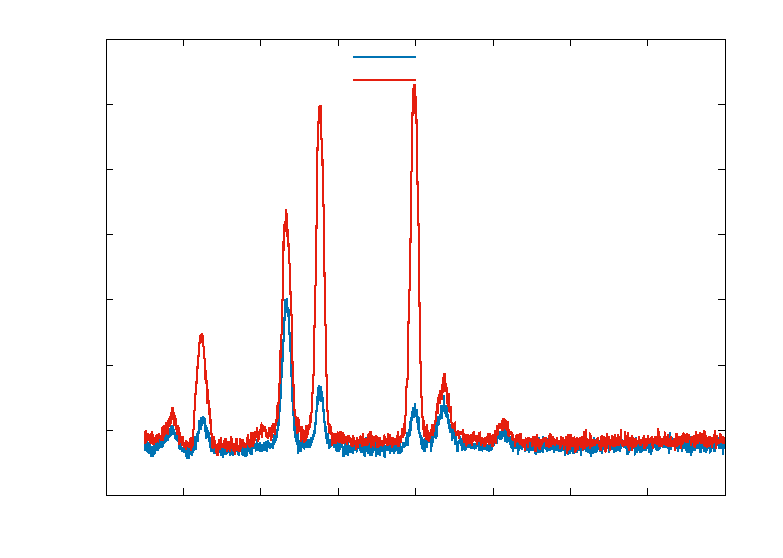
\includegraphics[width={360.00bp},height={252.00bp}]{Anhang/cdcl3_as}}%
    \gplfronttext
  \end{picture}%
\endgroup
}}
    \caption{Gemessene Plots für Deuterium Chlorophorm für $0^\circ$ und $90^\circ$-Polarisation im (Anti-)Stokes-Bereich}
\end{figure}\newpage
\section{Bromophorm}
\begin{figure}[h]
    \centering\subfigure[Stokes Linien]{\scalebox{0.94}{% GNUPLOT: LaTeX picture with Postscript
\begingroup
  % Encoding inside the plot.  In the header of your document, this encoding
  % should to defined, e.g., by using
  % \usepackage[cp1252,<other encodings>]{inputenc}
  \inputencoding{cp1252}%
  \makeatletter
  \providecommand\color[2][]{%
    \GenericError{(gnuplot) \space\space\space\@spaces}{%
      Package color not loaded in conjunction with
      terminal option `colourtext'%
    }{See the gnuplot documentation for explanation.%
    }{Either use 'blacktext' in gnuplot or load the package
      color.sty in LaTeX.}%
    \renewcommand\color[2][]{}%
  }%
  \providecommand\includegraphics[2][]{%
    \GenericError{(gnuplot) \space\space\space\@spaces}{%
      Package graphicx or graphics not loaded%
    }{See the gnuplot documentation for explanation.%
    }{The gnuplot epslatex terminal needs graphicx.sty or graphics.sty.}%
    \renewcommand\includegraphics[2][]{}%
  }%
  \providecommand\rotatebox[2]{#2}%
  \@ifundefined{ifGPcolor}{%
    \newif\ifGPcolor
    \GPcolorfalse
  }{}%
  \@ifundefined{ifGPblacktext}{%
    \newif\ifGPblacktext
    \GPblacktexttrue
  }{}%
  % define a \g@addto@macro without @ in the name:
  \let\gplgaddtomacro\g@addto@macro
  % define empty templates for all commands taking text:
  \gdef\gplbacktext{}%
  \gdef\gplfronttext{}%
  \makeatother
  \ifGPblacktext
    % no textcolor at all
    \def\colorrgb#1{}%
    \def\colorgray#1{}%
  \else
    % gray or color?
    \ifGPcolor
      \def\colorrgb#1{\color[rgb]{#1}}%
      \def\colorgray#1{\color[gray]{#1}}%
      \expandafter\def\csname LTw\endcsname{\color{white}}%
      \expandafter\def\csname LTb\endcsname{\color{black}}%
      \expandafter\def\csname LTa\endcsname{\color{black}}%
      \expandafter\def\csname LT0\endcsname{\color[rgb]{1,0,0}}%
      \expandafter\def\csname LT1\endcsname{\color[rgb]{0,1,0}}%
      \expandafter\def\csname LT2\endcsname{\color[rgb]{0,0,1}}%
      \expandafter\def\csname LT3\endcsname{\color[rgb]{1,0,1}}%
      \expandafter\def\csname LT4\endcsname{\color[rgb]{0,1,1}}%
      \expandafter\def\csname LT5\endcsname{\color[rgb]{1,1,0}}%
      \expandafter\def\csname LT6\endcsname{\color[rgb]{0,0,0}}%
      \expandafter\def\csname LT7\endcsname{\color[rgb]{1,0.3,0}}%
      \expandafter\def\csname LT8\endcsname{\color[rgb]{0.5,0.5,0.5}}%
    \else
      % gray
      \def\colorrgb#1{\color{black}}%
      \def\colorgray#1{\color[gray]{#1}}%
      \expandafter\def\csname LTw\endcsname{\color{white}}%
      \expandafter\def\csname LTb\endcsname{\color{black}}%
      \expandafter\def\csname LTa\endcsname{\color{black}}%
      \expandafter\def\csname LT0\endcsname{\color{black}}%
      \expandafter\def\csname LT1\endcsname{\color{black}}%
      \expandafter\def\csname LT2\endcsname{\color{black}}%
      \expandafter\def\csname LT3\endcsname{\color{black}}%
      \expandafter\def\csname LT4\endcsname{\color{black}}%
      \expandafter\def\csname LT5\endcsname{\color{black}}%
      \expandafter\def\csname LT6\endcsname{\color{black}}%
      \expandafter\def\csname LT7\endcsname{\color{black}}%
      \expandafter\def\csname LT8\endcsname{\color{black}}%
    \fi
  \fi
    \setlength{\unitlength}{0.0500bp}%
    \ifx\gptboxheight\undefined%
      \newlength{\gptboxheight}%
      \newlength{\gptboxwidth}%
      \newsavebox{\gptboxtext}%
    \fi%
    \setlength{\fboxrule}{0.5pt}%
    \setlength{\fboxsep}{1pt}%
\begin{picture}(7200.00,5040.00)%
    \gplgaddtomacro\gplbacktext{%
      \csname LTb\endcsname%%
      \put(726,440){\makebox(0,0)[r]{\strut{}$0.05$}}%
      \put(726,927){\makebox(0,0)[r]{\strut{}$0.1$}}%
      \put(726,1413){\makebox(0,0)[r]{\strut{}$0.15$}}%
      \put(726,1900){\makebox(0,0)[r]{\strut{}$0.2$}}%
      \put(726,2386){\makebox(0,0)[r]{\strut{}$0.25$}}%
      \put(726,2873){\makebox(0,0)[r]{\strut{}$0.3$}}%
      \put(726,3359){\makebox(0,0)[r]{\strut{}$0.35$}}%
      \put(726,3846){\makebox(0,0)[r]{\strut{}$0.4$}}%
      \put(726,4332){\makebox(0,0)[r]{\strut{}$0.45$}}%
      \put(726,4819){\makebox(0,0)[r]{\strut{}$0.5$}}%
      \put(858,220){\makebox(0,0){\strut{}$560$}}%
      \put(1601,220){\makebox(0,0){\strut{}$570$}}%
      \put(2344,220){\makebox(0,0){\strut{}$580$}}%
      \put(3087,220){\makebox(0,0){\strut{}$590$}}%
      \put(3831,220){\makebox(0,0){\strut{}$600$}}%
      \put(4574,220){\makebox(0,0){\strut{}$610$}}%
      \put(5317,220){\makebox(0,0){\strut{}$620$}}%
      \put(6060,220){\makebox(0,0){\strut{}$630$}}%
      \put(6803,220){\makebox(0,0){\strut{}$640$}}%
    }%
    \gplgaddtomacro\gplfronttext{%
      \csname LTb\endcsname%%
      \put(3102,4646){\makebox(0,0)[r]{\strut{}$0^\circ$ Polarisation}}%
      \csname LTb\endcsname%%
      \put(3102,4426){\makebox(0,0)[r]{\strut{}$90^\circ$ Polarisation}}%
    }%
    \gplbacktext
    \put(0,0){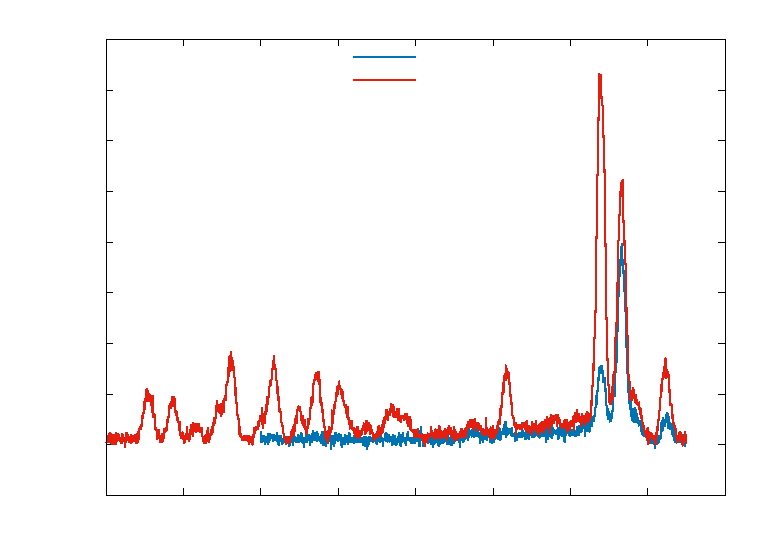
\includegraphics[width={360.00bp},height={252.00bp}]{Anhang/chbr3_s}}%
    \gplfronttext
  \end{picture}%
\endgroup
}}\\
    \subfigure[Anti-Stokes Linien]{\scalebox{0.94}{% GNUPLOT: LaTeX picture with Postscript
\begingroup
  % Encoding inside the plot.  In the header of your document, this encoding
  % should to defined, e.g., by using
  % \usepackage[cp1252,<other encodings>]{inputenc}
  \inputencoding{cp1252}%
  \makeatletter
  \providecommand\color[2][]{%
    \GenericError{(gnuplot) \space\space\space\@spaces}{%
      Package color not loaded in conjunction with
      terminal option `colourtext'%
    }{See the gnuplot documentation for explanation.%
    }{Either use 'blacktext' in gnuplot or load the package
      color.sty in LaTeX.}%
    \renewcommand\color[2][]{}%
  }%
  \providecommand\includegraphics[2][]{%
    \GenericError{(gnuplot) \space\space\space\@spaces}{%
      Package graphicx or graphics not loaded%
    }{See the gnuplot documentation for explanation.%
    }{The gnuplot epslatex terminal needs graphicx.sty or graphics.sty.}%
    \renewcommand\includegraphics[2][]{}%
  }%
  \providecommand\rotatebox[2]{#2}%
  \@ifundefined{ifGPcolor}{%
    \newif\ifGPcolor
    \GPcolorfalse
  }{}%
  \@ifundefined{ifGPblacktext}{%
    \newif\ifGPblacktext
    \GPblacktexttrue
  }{}%
  % define a \g@addto@macro without @ in the name:
  \let\gplgaddtomacro\g@addto@macro
  % define empty templates for all commands taking text:
  \gdef\gplbacktext{}%
  \gdef\gplfronttext{}%
  \makeatother
  \ifGPblacktext
    % no textcolor at all
    \def\colorrgb#1{}%
    \def\colorgray#1{}%
  \else
    % gray or color?
    \ifGPcolor
      \def\colorrgb#1{\color[rgb]{#1}}%
      \def\colorgray#1{\color[gray]{#1}}%
      \expandafter\def\csname LTw\endcsname{\color{white}}%
      \expandafter\def\csname LTb\endcsname{\color{black}}%
      \expandafter\def\csname LTa\endcsname{\color{black}}%
      \expandafter\def\csname LT0\endcsname{\color[rgb]{1,0,0}}%
      \expandafter\def\csname LT1\endcsname{\color[rgb]{0,1,0}}%
      \expandafter\def\csname LT2\endcsname{\color[rgb]{0,0,1}}%
      \expandafter\def\csname LT3\endcsname{\color[rgb]{1,0,1}}%
      \expandafter\def\csname LT4\endcsname{\color[rgb]{0,1,1}}%
      \expandafter\def\csname LT5\endcsname{\color[rgb]{1,1,0}}%
      \expandafter\def\csname LT6\endcsname{\color[rgb]{0,0,0}}%
      \expandafter\def\csname LT7\endcsname{\color[rgb]{1,0.3,0}}%
      \expandafter\def\csname LT8\endcsname{\color[rgb]{0.5,0.5,0.5}}%
    \else
      % gray
      \def\colorrgb#1{\color{black}}%
      \def\colorgray#1{\color[gray]{#1}}%
      \expandafter\def\csname LTw\endcsname{\color{white}}%
      \expandafter\def\csname LTb\endcsname{\color{black}}%
      \expandafter\def\csname LTa\endcsname{\color{black}}%
      \expandafter\def\csname LT0\endcsname{\color{black}}%
      \expandafter\def\csname LT1\endcsname{\color{black}}%
      \expandafter\def\csname LT2\endcsname{\color{black}}%
      \expandafter\def\csname LT3\endcsname{\color{black}}%
      \expandafter\def\csname LT4\endcsname{\color{black}}%
      \expandafter\def\csname LT5\endcsname{\color{black}}%
      \expandafter\def\csname LT6\endcsname{\color{black}}%
      \expandafter\def\csname LT7\endcsname{\color{black}}%
      \expandafter\def\csname LT8\endcsname{\color{black}}%
    \fi
  \fi
    \setlength{\unitlength}{0.0500bp}%
    \ifx\gptboxheight\undefined%
      \newlength{\gptboxheight}%
      \newlength{\gptboxwidth}%
      \newsavebox{\gptboxtext}%
    \fi%
    \setlength{\fboxrule}{0.5pt}%
    \setlength{\fboxsep}{1pt}%
\begin{picture}(7200.00,5040.00)%
    \gplgaddtomacro\gplbacktext{%
      \csname LTb\endcsname%%
      \put(594,440){\makebox(0,0)[r]{\strut{}$0$}}%
      \put(594,927){\makebox(0,0)[r]{\strut{}$0.1$}}%
      \put(594,1413){\makebox(0,0)[r]{\strut{}$0.2$}}%
      \put(594,1900){\makebox(0,0)[r]{\strut{}$0.3$}}%
      \put(594,2386){\makebox(0,0)[r]{\strut{}$0.4$}}%
      \put(594,2873){\makebox(0,0)[r]{\strut{}$0.5$}}%
      \put(594,3359){\makebox(0,0)[r]{\strut{}$0.6$}}%
      \put(594,3846){\makebox(0,0)[r]{\strut{}$0.7$}}%
      \put(594,4332){\makebox(0,0)[r]{\strut{}$0.8$}}%
      \put(594,4819){\makebox(0,0)[r]{\strut{}$0.9$}}%
      \put(726,220){\makebox(0,0){\strut{}$620$}}%
      \put(1594,220){\makebox(0,0){\strut{}$630$}}%
      \put(2462,220){\makebox(0,0){\strut{}$640$}}%
      \put(3330,220){\makebox(0,0){\strut{}$650$}}%
      \put(4199,220){\makebox(0,0){\strut{}$660$}}%
      \put(5067,220){\makebox(0,0){\strut{}$670$}}%
      \put(5935,220){\makebox(0,0){\strut{}$680$}}%
      \put(6803,220){\makebox(0,0){\strut{}$690$}}%
    }%
    \gplgaddtomacro\gplfronttext{%
      \csname LTb\endcsname%%
      \put(5816,4646){\makebox(0,0)[r]{\strut{}$0^\circ$ Polarisation}}%
      \csname LTb\endcsname%%
      \put(5816,4426){\makebox(0,0)[r]{\strut{}$90^\circ$ Polarisation}}%
    }%
    \gplbacktext
    \put(0,0){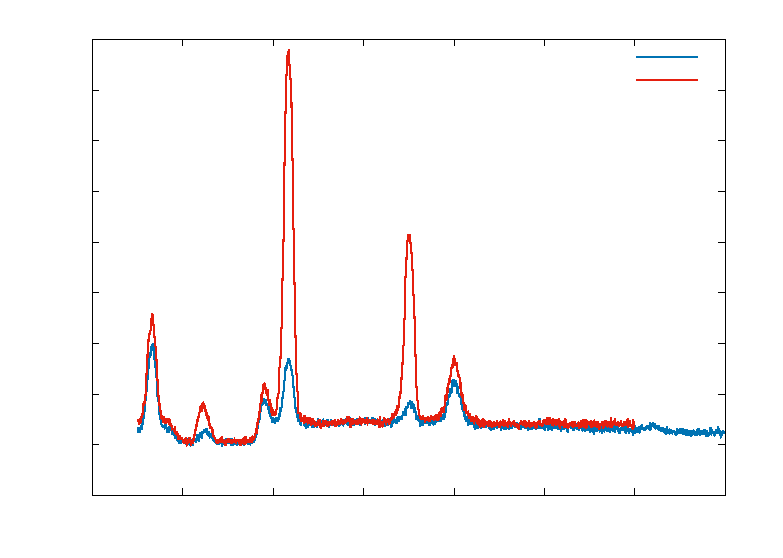
\includegraphics[width={360.00bp},height={252.00bp}]{Anhang/chbr3_as}}%
    \gplfronttext
  \end{picture}%
\endgroup
}}
    \caption{Gemessene Plots für Bromophorm für $0^\circ$ und $90^\circ$-Polarisation im (Anti-)Stokes-Bereich}
\end{figure}\newpage

    % Literatur
    \bibliographystyle{plainnat}
    \nocite{*}
    \bibliography{Auswertung.bib}

\end{document}